%% --------------------------------------------------------------------
%% Template UTEC Tesis
%% --------------------------------------------------------------------
% Este es el archivo que se debe compilar.
% 
% Este template ha sido modificado y actualizado por Eduardo Castro y Roosevelt Ubaldo en base a lo trabajado por Víctor Murray, Oscar Ramos y Juan Carlos Barbaran.
%
% Última actualización: Mayo, 2022

\documentclass[a4paper,12pt,oneside]{tesisutec}

\selectlanguage{spanish}

%% Paquetes
\usepackage[utf8]{inputenc}
\usepackage[square, numbers, comma, sort&compress]{natbib}
\usepackage{url}

% Libreria de idioma
\usepackage[spanish]{babel}
% Libreria para posicionamiento
\usepackage{float}
% Librerias para insertar codigos
\usepackage[spanish,onelanguage,ruled,vlined]{algorithm2e}
\usepackage{verbatim} 
% Librería para hipervínculos
\usepackage{hyperref}
 % Librería necesaria para arreglar el orden de referencias en overleaf.com
\usepackage{notoccite}

\usepackage{tabularx}

\hbadness=10000

% Incluir acá los paquetes adicionales que deseas. 
% Ubicación de los imágenes.
\graphicspath{images/}

\makeatletter
% Reinsert missing \algbackskip
\def\algbackskip{\hskip-\ALG@thistlm}
\makeatother

\hypersetup{urlcolor=blue, colorlinks=true}

\begin{document}

\frontmatter

\department{CIENCIA DE LA COMPUTACIÓN}
\degree{bachiller }
\major{Ciencia de la Computación}

\title{Análisis Comparativo del Client Drift en Arquitecturas CNN, ViT, SSM y Vision GNN bajo Aprendizaje Federado No-IID}

\author{Luis Fernando Méndez Lázaro \texorpdfstring{\orcid{0000-0000-0000-0000}}{}} % Es obligatorio
\supervisor{Victor Flores Benites \texorpdfstring{\orcid{0000-0000-0000-0000}}{}} % Es obligatorio
\date{2026}

\maketitle

\setstretch{1.5}


%% ============================================================================
%  Dedicatoria
%% ============================================================================

\dedicatory{
A mi familia, cuyo apoyo incondicional y amor han sido el pilar fundamental de mi trayectoria. A mis mentores y amigos, quienes me inspiraron a seguir aprendiendo y creciendo.
}

%% ============================================================================
%  Página de Agradecimientos
%% ============================================================================

\acknowledgements{

Quisiera expresar mi más sincero agradecimiento a mi asesor, cuya orientación y comentarios fueron invaluables durante el desarrollo de esta tesis. Asimismo, agradezco a mis profesores y compañeros por sus aportes, apoyo y aliento a lo largo de esta investigación.

}


\tableofcontents

\newpage

\listoftables

\newpage

\listoffigures

\addtocontents{toc}{\vspace{1.5em}}

%% ============================================================================
\mainmatter
\pagestyle{fancy}

\input{secciones/resumen}
\input{secciones/abstract} 
\customchapter{INTRODUCCI\'ON}

En los últimos años, el aprendizaje automático distribuido ha cobrado una importancia 
creciente debido al aumento de dispositivos conectados y a la gran cantidad de datos 
generados y almacenados por distintas organizaciones \cite{kairouz2021advances, mahmud2026survey}. 
Esta situación ha impulsado el desarrollo de modelos capaces de aprender a partir de información 
distribuida y de adaptarse a poblaciones con características diversas \cite{DBLP:journals/corr/abs-1908-07873}. 
Sin embargo, en sectores como la salud, la educación y las finanzas, el uso de estos datos está
limitado por normativas de privacidad como HIPAA (\textit{Health Insurance Portability and 
Accountability Act}) y GDPR (\textit{General Data Protection Regulation}), que restringen el 
intercambio de información sensible entre instituciones \cite{noor2026federated}. Frente a este 
desafío, el \textit{Federated Learning} (FL) se ha consolidado como una alternativa viable 
\cite{kairouz2021advances}, ya que permite entrenar modelos de manera local en cada entidad y 
compartir únicamente las actualizaciones de los parámetros con un servidor central encargado de 
combinarlas, evitando así la transferencia directa de los datos originales 
\cite{al2502principles,DBLP:journals/corr/McMahanMRA16}.


A pesar de su elegancia conceptual, el FL enfrenta un desafío fundamental en escenarios reales:
las distribuciones de datos locales difieren significativamente entre clientes, ya sea por 
diferencias en las poblaciones atendidas, en los protocolos de recolección o en los equipos 
utilizados. Esta condición, conocida como \textit{non-IID} (\textit{non-Independent and 
Identically Distributed}), viola el supuesto de homogeneidad subyacente a los análisis de 
convergencia originales del FL. Su consecuencia directa es el fenómeno central que motiva 
esta investigación: el \textit{client drift} \cite{DBLP:journals/corr/abs-1910-06378}. 
Durante el entrenamiento local sobre datos sesgados, el modelo de cada cliente converge hacia 
un óptimo local que puede encontrarse significativamente alejado de la solución global. A 
medida que avanzan las rondas de comunicación, esta divergencia acumulada genera actualizaciones 
que, al promediarse en el servidor, ubican al modelo global en una región de alta pérdida para 
todos los participantes. El resultado es que el progreso de aprendizaje obtenido en cada ronda 
se anula sistemáticamente \cite{seo2025understanding}.


La comunidad investigadora ha respondido a este problema principalmente mediante el desarrollo 
de algoritmos de agregación más robustos, como FedProx \cite{DBLP:journals/corr/abs-1812-06127}, 
SCAFFOLD \cite{DBLP:journals/corr/abs-1910-06378} y sus variantes, que incorporan términos de 
regularización o mecanismos de corrección de varianza para contener la divergencia entre clientes. 
Estos enfoques han logrado mejoras sustanciales en escenarios de heterogeneidad moderada, pero 
su efectividad depende de supuestos sobre el paisaje de pérdida del modelo que no siempre se cumplen 
en la práctica. En particular, la relación entre la \textit{arquitectura} del modelo y la severidad 
con que se manifiesta el \textit{client drift} ha recibido atención considerablemente menor 
\cite{qu2022rethinking, siomos2024architecture}, pese a ser una variable de diseño que los 
profesionales deben definir antes de cualquier elección algorítmica.


Las \textit{Convolutional Neural Networks} (CNNs) explotan filtros espaciales locales; los 
\textit{Vision Transformers} (ViTs) emplean mecanismos de autoatención global; los 
\textit{State-Space Models} (SSMs) modelan dependencias mediante transiciones de estado sobre 
secuencias de parches de la imagen; y los \textit{Vision Graph Neural Networks} (Vision GNNs) 
propagan información mediante mensajes entre regiones de la imagen organizadas en grafos. Estas 
diferencias en los sesgos inductivos implican que cada familia procesa la información de entrada 
de formas radicalmente distintas, lo que debería traducirse en perfiles de drift igualmente 
distintos bajo condiciones de federación heterogénea. Sin embargo, hasta la fecha no existen 
estudios que hayan caracterizado sistemáticamente cómo estas diferencias arquitectónicas se 
manifiestan a nivel de capa a lo largo de las rondas de comunicación, bajo protocolos 
experimentales controlados y comparables entre familias.


Una parte importante de esta brecha es la relacionada con las estrategias de normalización. 
Las CNNs convencionales dependen de la \textit{Batch Normalization} (BN), cuya 
estabilidad requiere estadísticas de mini-batch representativas de la distribución conjunta de 
los datos \cite{DBLP:journals/corr/abs-1803-08494}. En un entorno federado con datos non-IID, 
cada cliente computa estas estadísticas sobre un subconjunto sesgado y reducido, lo que introduce 
una discrepancia entre las estadísticas locales y las globales. Esta discrepancia se propaga 
durante la agregación y puede dominar el comportamiento de convergencia de todo el modelo 
\cite{du2022rethinking}. Por el contrario, las estrategias de normalización independientes del 
tamaño del batch, como \textit{Layer Normalization} (LN) y \textit{Group Normalization} (GN), 
no dependen de las estadísticas entre clientes y se espera que sean inherentemente más estables 
en este contexto \cite{wang2023batch, casella2023experimentingnormalizationlayersfederated}. 
Esta diferencia sugiere que parte de la inestabilidad observada en las CNNs federadas podría 
ser atribuible a la normalización, y no al sesgo inductivo convolucional en sí mismo, pero esta 
hipótesis no ha sido verificada empíricamente a nivel de capa de forma sistemática.


Frente a esta situación, esta investigación propone una caracterización empírica a nivel de capa 
del \textit{client drift} en cuatro familias arquitectónicas de visión: EfficientNet-B1 como 
representante de las CNNs, ViT-Tiny como representante de los Vision Transformers, Vim-Tiny como 
representante de los State-Space Models, y ViG-Tiny (\textit{Vision GNN}) como representante de 
los modelos basados en grafos. Todas las arquitecturas son evaluadas a escala de parámetros 
comparable, bajo condiciones de federación idénticas, en dos conjuntos de datos complementarios: 
Brain Tumor MRI, que representa un escenario realista de imagenología médica con heterogeneidad 
natural entre instituciones, y CIFAR-10, que constituye un punto de referencia estándar en la 
literatura de FL. El grado de heterogeneidad no-IID es controlado mediante particiones de 
Dirichlet con $\alpha \in \{1000.0, 1.0, 0.3, 0.1, 0.03\}$, y se evalúan dos algoritmos de 
agregación: FedAvg y FedProx.


Para caracterizar el drift, se emplean tres métricas complementarias registradas por capa y por 
ronda de comunicación. La divergencia de pesos ($L_2$) mide la distancia entre los parámetros 
locales de cada cliente y el modelo global antes de la agregación, cuantificando la magnitud del 
drift acumulado por tipo de capa. La alineación de gradientes (similitud coseno entre pares de 
clientes) evalúa si las direcciones de actualización de distintos participantes son constructivas 
o destructivas, identificando las capas con mayor interferencia entre clientes durante la 
agregación. El \textit{Centered Kernel Alignment} (CKA) \cite{DBLP:journals/corr/abs-1905-00414} 
compara las representaciones internas aprendidas entre clientes a lo largo del entrenamiento, 
permitiendo determinar si el drift en los pesos se traduce en una divergencia funcional en las 
representaciones, o si los modelos convergen a representaciones similares a pesar de la 
disparidad paramétrica. La combinación de estas tres métricas permite desarrollar un perfil de 
deriva (\textit{drift profile}) para cada arquitectura.


Adicionalmente, se realiza una ablación de normalización sobre EfficientNet, reemplazando su 
BatchNorm por GroupNorm y LayerNorm, con el objetivo de determinar si la inestabilidad federada 
observada en las CNNs es atribuible a la divergencia de estadísticas de lote —un efecto propio 
de la normalización— o al sesgo inductivo convolucional como factor independiente.


Se espera que esta investigación contribuya con: (1) la primera caracterización empírica 
transversal entre familias CNN, ViT, SSM y Vision GNN, con granularidad por capa, sobre cómo 
los sesgos inductivos modulan el \textit{client drift} bajo condiciones non-IID controladas; y 
(2) la incorporación de CKA como métrica de análisis representacional que complementa las medidas 
paramétricas existentes, permitiendo distinguir entre drift en pesos y divergencia funcional en 
las representaciones. Adicionalmente, se aportan: (3) una ablación de normalización que disocia 
la inestabilidad de BatchNorm del sesgo inductivo convolucional; y (4) recomendaciones prácticas, 
fundamentadas en evidencia empírica a nivel de capa, para la selección de arquitecturas y 
estrategias de normalización en escenarios de FL con datos heterogéneos.


\introsection{Descripci\'on del problema}

% -----------------------------------------------------------------------
% CAMBIO: "mecanismos de selección de contenido secuenciales" →
% "transiciones de estado sobre secuencias de parches de la imagen"
% (consistencia con la intro general y más intuitivo para visión).
% "filtrar características" → "privilegiar características"
% ("filtrar" era ambiguo: podía leerse como seleccionar o descartar).
% "practicantes" → "profesionales".
% -----------------------------------------------------------------------
A pesar de su relevancia práctica, la literatura no ha examinado sistemáticamente 
cómo la arquitectura del modelo influye en el \textit{client drift} durante el entrenamiento 
federado con datos heterogéneos \cite{pieri2023handlingdataheterogeneityarchitectural, li2023fedtp}. 
La investigación existente ha abordado este problema casi exclusivamente desde la perspectiva 
del algoritmo de agregación \cite{siomos2024architecture}, asumiendo implícitamente que la 
arquitectura es un factor neutral. Sin embargo, la manera en que cada familia arquitectónica 
procesa la información local determina de forma directa cuánto y de qué manera diverge el 
modelo local del modelo global a lo largo de las rondas de comunicación.

Las CNNs procesan la información mediante filtros locales con pesos compartidos y dependen de 
estadísticas de mini-batch para su normalización, lo que las expone al sesgo local de los datos 
y a la incompatibilidad de estadísticas entre clientes. Los Vision Transformers procesan la 
imagen mediante autoatención global, lo que puede derivar en cabezales de atención fuertemente 
especializados hacia las clases locales bajo distribuciones heterogéneas. Los State-Space Models 
modelan dependencias espaciales mediante transiciones de estado sobre secuencias de parches de 
la imagen; bajo distribuciones non-IID, dichos mecanismos podrían aprender a privilegiar 
características representativas de las clases locales, acumulando sesgo progresivamente a lo 
largo de la secuencia de parches. Los Vision GNNs construyen grafos dinámicos sobre regiones 
de la imagen y propagan información mediante mensajes entre nodos; bajo distribuciones 
heterogéneas, la topología del grafo local podría divergir sistemáticamente entre clientes, 
amplificando el \textit{drift} a través de las capas de propagación. Estos mecanismos 
distintos sugieren que el \textit{drift} varía entre familias no solo en 
magnitud, sino también en su distribución interna por capas y representaciones aprendidas.

A pesar de estas diferencias, no existe un estudio que compare sistemáticamente cómo estas cuatro 
familias experimentan el \textit{client drift}, cómo la 
divergencia se distribuye entre los distintos tipos de capas dentro de cada arquitectura, y 
si la divergencia paramétrica se traduce en una divergencia representacional medible mediante 
CKA. Esta ausencia limita la capacidad de los profesionales de FL para tomar decisiones 
informadas sobre la arquitectura más apropiada para un escenario dado, y restringe el diseño 
de estrategias de agregación que aprovechen la estructura específica del modelo.


\introsection{Justificaci\'on}

La presente investigación responde a una necesidad concreta en el campo del aprendizaje 
federado aplicado a visión por computadora: comprender cómo la elección de arquitectura 
afecta la estabilidad del entrenamiento distribuido bajo condiciones de heterogeneidad 
estadística. Desde una perspectiva científica, contribuye con evidencia empírica que permite 
distinguir entre el efecto del sesgo inductivo y el efecto de la estrategia de normalización 
sobre el \textit{drift}, dos factores que la literatura ha tratado de manera conjunta sin 
separarlos experimentalmente. La incorporación de CKA como métrica complementaria representa 
además un aporte metodológico que enriquece el marco de análisis disponible para estudiar la 
evolución de representaciones internas en sistemas federados.

Desde una perspectiva aplicada, los resultados de esta investigación tienen implicaciones 
directas para cualquier organización que deba implementar FL en entornos con datos heterogéneos 
(como centros de salud, sistemas educativos distribuidos o redes de sensores industriales). 
En estos contextos, seleccionar una arquitectura de visión sin evidencia sobre su comportamiento 
bajo heterogeneidad estadística implica un riesgo de diseño no trivial. Los perfiles de 
\textit{drift} por familia arquitectónica, combinados con los resultados de la ablación de 
normalización, proporcionarán recomendaciones concretas para esas decisiones de diseño.


\introsection{Objetivos}


\introsubsection{Objetivo general}

Desarrollar y comparar perfiles de \textit{drift} a nivel de capa para las familias CNN, 
ViT, SSM y Vision GNN bajo condiciones de federación non-IID controladas, con el fin de 
identificar cómo los sesgos inductivos de cada familia modulan la divergencia de parámetros, 
la alineación de gradientes y la similitud de representaciones internas durante el 
entrenamiento federado.


\introsubsection{Objetivos espec\'ificos}

\begin{enumerate}
    \item \sloppy Medir la divergencia de pesos ($L_2$) por tipo de capa para EfficientNet-B1, 
    ViT-Tiny, Vim-Tiny y ViG-Tiny bajo particiones Dirichlet con 
    $\alpha \in \{1000.0, 1.0, 0.3, 0.1, 0.03\}$, empleando FedAvg y FedProx sobre los 
    conjuntos de datos Brain Tumor MRI y CIFAR-10.

    \item Evaluar la alineación de gradientes entre pares de clientes mediante similitud 
    coseno por capa, identificando las familias y tipos de capa más propensos a interferencia 
    destructiva durante la agregación.

    \item Analizar la evolución de las representaciones internas de cada arquitectura mediante 
    CKA entre pares de clientes a lo largo de las rondas de comunicación, determinando si el 
    \textit{drift} paramétrico implica necesariamente una divergencia funcional en las 
    representaciones aprendidas.

    \item Aislar la contribución de la estrategia de normalización al \textit{drift} 
    observado en EfficientNet mediante una variante experimental que sustituye BatchNorm 
    por GroupNorm y LayerNorm, manteniendo fija la arquitectura base y la configuración 
    de federación.

    \item Formular recomendaciones prácticas para la selección de arquitecturas y estrategias 
    de normalización en escenarios de FL con datos heterogéneos, fundamentadas en los perfiles 
    de \textit{drift} empíricos obtenidos.
\end{enumerate}
\chapter{REVISI\'ON CR\'ITICA DE LA LITERATURA}

Este capítulo revisa críticamente el estado del arte en las líneas temáticas que estructuran esta 
investigación: estudios comparativos de arquitecturas de visión bajo condiciones
federadas heterogéneas, el papel de la arquitectura como variable de diseño en FL, la integración
de modelos basados en State Space Models (SSM/Mamba) y de Vision GNNs en sistemas federados,
y los enfoques de análisis por capas que fundamentan las métricas de drift adoptadas.
El objetivo no es enumerar estudios, sino identificar tendencias, vacíos y la cadena de conocimiento
que justifica las decisiones metodológicas de esta tesis.


\section{Estudios comparativos de arquitecturas de visión en FL}

La pregunta de si la elección de arquitectura afecta de forma sistemática el comportamiento de los
modelos bajo condiciones no-IID fue formulada con rigor por primera vez por Qu et al.\
\cite{qu2022rethinking}, en lo que constituyó la primera investigación empírica exhaustiva de
múltiples familias arquitectónicas bajo distintos algoritmos federados, \textit{benchmarks} reales
y particiones heterogéneas.
Sus experimentos, que abarcaron CNNs (ResNet, EfficientNet) y Vision Transformers (ViT, Swin)
sobre CIFAR-10, Retina y CelebA, evidenciaron que las arquitecturas basadas en autoatención eran
sistemáticamente más robustas ante \textit{distributional shifts} no-IID, con mejoras de hasta 37
puntos porcentuales sobre las CNNs equivalentes bajo alta heterogeneidad.
Los autores argumentaron que el mecanismo de autoatención global, al no depender de estadísticas
de mini-batch locales para su normalización, mitigaba de forma inherente la divergencia entre
actualizaciones de distintos clientes.
Sin embargo, el trabajo no desagregaba las fuentes de esa ventaja: no se distinguía entre el
efecto del sesgo inductivo (convolución local frente a atención global) y el efecto de la estrategia
de normalización (BatchNorm en CNNs frente a LayerNorm en ViTs), ni se proporcionaba ningún
análisis por capa que permitiera localizar dónde se concentraba la divergencia.

En la misma dirección, Zuo et al.\ \cite{zuo2022empirical} realizaron una comparación temprana
entre CNNs ligeras y variantes compactas de ViT bajo restricciones de memoria y tiempo propias
de dispositivos de borde, confirmando que los ViTs entrenados desde cero con imágenes de baja
resolución podían superar a sus homólogos CNN en precisión global tanto en escenarios IID como
no-IID con un coste computacional comparable.
No obstante, el estudio operó exclusivamente a nivel de métricas de rendimiento final, sin
descomponer el comportamiento por capa ni explorar el efecto de la normalización.

Las comparaciones más recientes han ido ampliando progresivamente el espectro de arquitecturas
evaluadas.
Büyüktaş et al.\ \cite{buyuktacs2024transformer} examinaron arquitecturas del estilo MetaFormer
---MLP-Mixer, ConvMixer y PoolFormer--- frente a ResNet-50 en clasificación multietiqueta de
teledetección bajo FL con FedAvg y MOON.
Bajo alta heterogeneidad, PoolFormer superó a ResNet-50 en 12.53 puntos de F1, mientras que MOON
apenas mejoró a las arquitecturas Transformer, lo que sugería que su robustez intrínseca ante el
drift reducía el beneficio marginal de los algoritmos de regularización contrastiva.
Li et al.\ \cite{li2025comparison} obtuvieron conclusiones análogas al comparar ViT-Base con
ResNet-50 en reconocimiento de acciones humanas bajo FL: el ViT federado alcanzó 87.30\% de
precisión frente al 79.29\% del ResNet, con una brecha de generalización cuatro veces menor,
atribuida al desarrollo de capacidad de abstracción transversal a los clientes a través del
mecanismo de autoatención.

Jiménez-Gutiérrez et al.\ \cite{jimenez2503thorough} aportaron una de las evaluaciones más
sistemáticas sobre el impacto diferencial de los tipos de heterogeneidad no-IID.
Mediante la Distancia de Hellinger como métrica unificada, demostraron que el sesgo de etiquetas
producía caídas de precisión de entre 10 y 40 puntos sobre la línea base centralizada, con umbrales
críticos de degradación a $\text{HD} > 0.5$ y $\text{HD} > 0.75$, mientras que los sesgos de
cantidad y características resultaban prácticamente inocuos.
Los modelos de transferencia como EfficientNet-B0 mostraron mayor sensibilidad al sesgo de etiquetas
que las CNNs entrenadas desde cero, y ninguno de los cinco algoritmos de agregación evaluados
---FedAvg, FedProx, MOON, POC y selección aleatoria--- logró reducir la brecha de forma sustancial
bajo alta heterogeneidad.
Este resultado constituye un punto de referencia empírico directo para la presente investigación:
los valores $\alpha \in \{1000.0, 1.0, 0.3, 0.1, 0.03\}$ empleados en las particiones de Dirichlet
se corresponden aproximadamente con los niveles HD analizados en dicho trabajo, y la incapacidad
algorítmica para resolver el problema bajo alta heterogeneidad refuerza la motivación de examinar
la arquitectura como variable independiente.
Sin embargo, el estudio se limitó exclusivamente a CNNs y no incorporó análisis por capas,
familias Transformer, SSMs ni Vision GNNs.

Estudios comparativos más recientes que incluyen SSMs han aportado evidencia complementaria,
aunque en entornos centralizados.
Biswas et al.\ \cite{biswas2025comparative} compararon diecisiete modelos de tres familias
---CNN, Transformer y SSM (Vision Mamba)--- en tres dominios de imágenes, concluyendo que los
modelos CNN alcanzaban mayor precisión bruta mientras que los basados en Mamba presentaban la
menor huella de memoria y la convergencia más rápida.
Yanar et al.\ \cite{yanar2025comparative} llegaron a una conclusión más matizada en el dominio
de rayos X de tórax: los modelos híbridos CNN-Transformer (ConvFormer, CaFormer) y EfficientNet
superaron consistentemente a las variantes de Mamba (MedMamba, VMamba) en 14 categorías de
patologías, advirtiendo que la competitividad de los SSMs no es universal y depende del dominio.
Ambos estudios se desarrollaron en entornos centralizados, sin federación ni análisis de drift,
por lo que sus conclusiones no son directamente transferibles a escenarios no-IID.

En el dominio de imagenología cerebral, varios estudios han aplicado arquitecturas de visión sobre
el dataset Brain Tumor MRI.
Trabajos como los de Chen et al.\ \cite{chenfederated} y Lai et al.\ \cite{lai2025advancing}
realizaron el entrenamiento de forma centralizada.
Quienes sí incorporaron FL ---Anoosha y Seetharamulu \cite{anoosha2025federated}, Zhou et al.\
\cite{zhou2024distributedfederatedlearningbaseddeep} y Appasami y Savarimuthu
\cite{appasami2025federated}--- lo hicieron empleando exclusivamente variantes CNN, sin realizar
ningún análisis de comportamiento por capas ni comparación entre familias arquitectónicas.
Ninguno de estos estudios abordó la dinámica de drift paramétrico o representacional a lo largo
de las rondas de comunicación.

En conclusión, los trabajos previos presentan las siguientes limitaciones: primero, las evaluaciones se centran predominantemente en métricas de rendimiento
final, sin medir los procesos internos que las generan; segundo,
el espacio arquitectónico comparado raramente ha superado dos familias de modelos, ignorando sistemáticamente los SSMs
y los Vision GNNs en contextos federados; y tercero, la heterogeneidad ha sido poco estudiada como un parámetro controlado que permita comparaciones rigurosas.
La presente investigación responde a las tres limitaciones de forma directa.


\section{Arquitectura como variable de diseño en FL}

El trabajo de Pieri et al.\ \cite{pieri2023handlingdataheterogeneityarchitectural} representa el
estudio de mayor alcance en términos de diversidad arquitectónica evaluada dentro de un marco
federado.
En él se compararon 19 modelos pertenecientes a cinco familias ---CNNs, Transformers, MLP-Mixers,
modelos híbridos y MetaFormers--- sobre cuatro conjuntos de datos FL con distintos tipos de
heterogeneidad, evaluando además el efecto ortogonal de cuatro algoritmos de optimización:
FedAvg, FedAVGM, FedProx y SCAFFOLD.
Los autores reportaron que las arquitecturas tipo MetaFormer (CAFormer, ConvFormer, PoolFormer)
exhibían la mayor robustez ante distribuciones heterogéneas, y que el cambio de arquitectura
producía mejoras más consistentes y de mayor magnitud que la elección del algoritmo de agregación.
El hallazgo más relevante para la presente investigación fue la ablación de normalización: al
sustituir BatchNorm por LayerNorm en modelos CNN, la brecha de rendimiento entre CNNs y
Transformers se reducía de forma considerable, sugiriendo que BatchNorm ---y no el sesgo
inductivo convolucional \textit{per se}--- era el factor determinante de la inferioridad de las
CNNs bajo FL heterogéneo.
Sin embargo, el trabajo presentó dos vacíos fundamentales: no incluyó ninguna arquitectura SSM
ni Vision GNN, y no incorporó métricas de drift paramétrico o representacional por capa.

Xu et al.\ \cite{xu2023fedconv} ofrecieron una perspectiva complementaria: mediante ablación
sistemática sobre componentes micro-arquitectónicos de una CNN pura, demostraron que con
modificaciones dirigidas ---función de activación SiLU, entrenamiento libre de normalización con
\textit{Adaptive Gradient Clipping}, \textit{stem} convolucional solapado y \textit{kernels}
de tamaño 9--- la arquitectura resultante (FedConv) superaba a ViT-Small en precisión FL bajo
alta heterogeneidad.
Este hallazgo matizó la conclusión de Qu et al.: la inferioridad de las CNNs no era inherente a
la convolución, sino que derivaba de decisiones micro-arquitectónicas corregibles, siendo la
eliminación de BatchNorm la modificación de mayor impacto individual.
No obstante, FedConv evaluó únicamente métricas de precisión y eficiencia de comunicación, sin
medir la divergencia de pesos por capa ni la alineación de gradientes entre clientes.

Siomos et al.\ \cite{siomos2024architecture} profundizaron en la dirección
\textit{normalization-free} mediante ANFR, una arquitectura que combina \textit{Scaled Weight
Standardization} (SWS) con mecanismos de atención de canal.
Al estandarizar los pesos en lugar de las activaciones, ANFR eliminó la dependencia del paso
hacia adelante de las estadísticas de mini-batch del cliente, logrando coherencia de los
descriptores de canal entre participantes heterogéneos.
Evaluada bajo siete algoritmos de agregación y cinco conjuntos de datos, ANFR alcanzó el mejor
rendimiento en todas las configuraciones, incluyendo escenarios de privacidad diferencial donde
otras estrategias de normalización degradaban fuertemente.
El trabajo confirmó que BatchNorm era el principal vector de inestabilidad federada en CNNs,
proporcionando base empírica sólida para la ablación de normalización planteada en esta tesis.
Sin embargo, como en el caso de Pieri et al. \cite{pieri2023handlingdataheterogeneityarchitectural}, el estudio se restringió a CNNs y no realizó
mediciones de drift por capa, gradiente o representación.

En conjunto, existe evidencia que la arquitectura es un eje de diseño primario en FL,
potencialmente más determinante que la elección del algoritmo de agregación, e identificó a
BatchNorm como el principal confusor entre el efecto del sesgo inductivo y el de la normalización.
No obstante, todos los estudios midieron el impacto arquitectónico exclusivamente a través de
precisión final, ninguno trazó la evolución del drift con granularidad por capa, y ninguno
extendió el análisis a las familias SSM o Vision GNN.


\section{State Space Models y Vision Mamba en FL}

Los modelos de espacio de estados selectivos irrumpieron en el dominio de la visión por computadora
con Vision Mamba (Vim) \cite{zhu2024vision}, que introdujo un bloque SSM bidireccional capaz de
procesar secuencias de parches de imagen con complejidad lineal en memoria y tiempo.
En comparación directa con DeiT, Vim-Tiny superó al Transformer equivalente en ImageNet-1K en
3.9 puntos de \textit{top-1 accuracy}, alcanzando una velocidad 2.8$\times$ mayor y un consumo
de memoria 86.8\% inferior a resoluciones elevadas.
El diseño emplea LayerNorm al inicio de cada bloque ---en contraste con la BatchNorm de las CNNs
clásicas---, lo que lo sitúa, desde la perspectiva de la normalización, en una posición análoga a
los ViTs.
La naturaleza secuencial del SSM implica, no obstante, un mecanismo de integración de la
información fundamentalmente distinto al de la autoatención: mientras los ViTs establecen
dependencias globales simultáneas entre todos los parches, los SSMs integran la información a
través de transiciones de estado selectivas dependientes del contenido, cuyo comportamiento bajo
distribuciones de clases heterogéneas entre clientes no había sido caracterizado.

La idoneidad de los SSMs para tareas de visión fue matizada por Yu y Wang \cite{yu2025mambaout},
quienes demostraron que MambaOut ---un modelo que elimina el componente SSM reemplazándolo por
convoluciones \textit{depthwise} con \textit{kernel} grande--- superaba a todas las variantes
visuales de Mamba en clasificación de ImageNet-1K, aunque no en tareas densas.
Los autores argumentaron que la clasificación estándar no satisface las condiciones de secuencia
larga ni de procesamiento autorregresivo para las cuales el SSM fue diseñado.
En el entorno federado, donde el mini-batch local puede ser reducido y la distribución de clases
local puede ser muy sesgada, no está claro \textit{a priori} si el mecanismo SSM aportará ventajas
o desventajas en términos de drift paramétrico y representacional.

En el dominio médico, MedMamba \cite{yue2024medmamba} y la revisión de Bansal et al.\
\cite{bansal2024comprehensive} documentaron que las variantes híbridas SSM-CNN ofrecen rendimiento
competitivo en clasificación de imágenes de múltiples modalidades, aunque en entornos centralizados.
La integración de Mamba en FL fue abordada por primera vez por Wu \cite{wu2024mamba}, quien
demostró mayor precisión y eficiencia de entrenamiento respecto a \textit{baselines} convolucionales,
concluyendo que los SSMs eran viables para aplicaciones distribuidas y sensibles a la privacidad.
No obstante, el estudio no exploró particiones no-IID sistematizadas ni ofreció análisis de drift
por capa.
Trabajos posteriores como los de Chen \cite{chen2024mamaba} y Guo et al.\ \cite{guo2026mamba}
aplicaron Mamba en FL a dominios específicos ---detección de rayos X y diagnóstico fotovoltaico,
respectivamente--- con el mismo foco en precisión final y sin estudiar los mecanismos de divergencia
paramétrica inducidos por la heterogeneidad.
La comprensión del comportamiento de los SSMs ante condiciones no-IID controladas, con análisis
por capa y a lo largo de las rondas de comunicación, permanece como un vacío no abordado.


\section{Vision GNNs en FL}

Los modelos de redes neuronales en grafos se originaron como herramientas para el procesamiento
de datos estructurados de forma irregular \cite{Gori2005ANM, Scarselli:2009ku}.
Han et al.\ \cite{han2022vision} introdujeron Vision GNN (ViG), la primera arquitectura de visión
pura basada en grafos para clasificación de imágenes a escala de ImageNet, demostrando que el
mecanismo de propagación de mensajes sobre un grafo de parches podía aprender representaciones
competitivas con las obtenidas por CNNs y ViTs.
El sesgo inductivo de ViG es cualitativamente distinto: mientras las CNNs explotan la localidad
espacial mediante filtros compartidos y los ViTs establecen dependencias globales a través de la
autoatención, ViG construye dinámicamente una topología de conectividad entre regiones de la imagen
y refina las representaciones nodales iterativamente, lo que puede resultar en una sensibilidad
diferente a la distribución de clases local de cada cliente bajo federación.

La interacción entre GNNs y FL fue sistematizada por He et al.\ \cite{DBLP:journals/corr/abs-2104-07145},
quienes presentaron FedGraphNN como la primera plataforma de \textit{benchmarking} para FL con
GNNs sobre datos nativamente graficados, abarcando 36 conjuntos de datos en siete dominios.
Sus experimentos revelaron que el rendimiento federado era sistemáticamente inferior al centralizado
y que la arquitectura GNN con mejor desempeño centralizado no mantenía necesariamente su ventaja
bajo federación ---resultado que anticipa la relevancia de estudiar el efecto moderador de la
arquitectura también para modelos basados en grafos.
Sin embargo, FedGraphNN operó exclusivamente sobre datos estructurados como grafos (moléculas,
redes de citas, sistemas de recomendación), sin considerar \textit{backbones} de visión sobre
imágenes.
Plataformas más recientes como FedGraph \cite{yao2024fedgraph} ampliaron la infraestructura
disponible pero mantuvieron el foco en eficiencia y seguridad del software, sin estudiar los
mecanismos de drift paramétrico o representacional.

La revisión sistemática de Shaikh y Samet \cite{shaikh2025federated} proporcionó una taxonomía
de la heterogeneidad en FedGNNs e identificó la heterogeneidad estructural/topológica como el
tipo más descuidado en la literatura, confirmando la ausencia de métricas estandarizadas para
cuantificar la no-IID-ness en grafos.
Más relevante para esta tesis, el survey no incluyó ningún estudio que empleara el \textit{backbone}
de Vision GNN en tareas de clasificación de imágenes bajo FL.
El trabajo de Cui et al.\ \cite{cui2025fedvig} fue el primero en integrar explícitamente una
arquitectura Vision GNN en un marco federado (FedVIG), empleando perturbación de datos mediante
modelos de difusión y aprendizaje contrastivo estructural para mejorar la generalización y la
privacidad.
Sin embargo, el trabajo no estudió el comportamiento del modelo ante particiones no-IID
sistematizadas, y su foco primario fue la privacidad, no la caracterización del drift.
Estudios que emplearon GNNs sobre el dataset de tumores cerebrales, como los de Gürsoy y Kaya
\cite{gursoy2024brain} o Elhamzi y Mokni \cite{elhamzi2026braingraphnet}, lo hicieron en entornos
centralizados con modelos híbridos o variantes de GCN ---no el \textit{backbone} de Vision GNN---
y sin ninguna consideración federada.

En consecuencia, la literatura no contiene ningún estudio que analice el comportamiento de Vision
GNN bajo datos heterogéneos en un entorno federado, ni que compare Vision GNN con Vision Mamba
en ese contexto.
Este vacío ---la ausencia de análisis de drift para Vision GNN bajo FL y la inexistencia de
comparaciones entre las cuatro familias (CNN, ViT, SSM, GNN) bajo condiciones no-IID controladas---
representa la brecha central que aborda la presente investigación.


\section{Análisis por capas y métricas de drift}

La evidencia empírica que motivó el análisis granular del drift provino inicialmente de trabajos
que utilizaron el Centered Kernel Alignment (CKA) como herramienta de diagnóstico representacional.
Son et al.\ \cite{son2022comparisons} fueron los primeros en aplicar CKA en un contexto de FL,
realizando experimentos con una CNN de siete capas y ResNet-50 bajo condiciones IID para identificar
qué capas exhibían similitud inter-cliente natural.
Sus resultados confirmaron que las capas tempranas convergían espontáneamente a representaciones
similares entre clientes incluso sin regularización explícita, mientras que las capas finales
---especialmente el clasificador--- mostraban alta disimilitud inter-cliente.
A partir de esta observación, propusieron FedCKA, un método que añade una penalización de
regularización basada en CKA únicamente sobre las capas naturalmente similares, con una eficiencia
computacional casi constante respecto de la profundidad de la red.
El trabajo estableció dos contribuciones metodológicas directamente relevantes para esta tesis:
la validación de CKA como métrica de divergencia representacional en FL y la constatación empírica
de que el drift no es uniforme a lo largo de la profundidad de la red.
Sin embargo, el análisis se realizó solo bajo IID como línea base y únicamente sobre arquitecturas
CNN, sin explorar cómo varían estos patrones entre familias arquitectónicas distintas ni bajo
diferentes niveles de heterogeneidad no-IID.

La base teórica del CKA lineal fue formalizada por Kornblith et al.\ \cite{DBLP:journals/corr/abs-1905-00414},
quienes demostraron que la métrica CKA es invariante a transformaciones ortogonales e isotropías de escala, propiedad fundamental para comparar representaciones aprendidas de forma independiente por distintos clientes.
Esta invarianza hace del CKA lineal el candidato natural para comparar las representaciones
internas de los modelos locales entre sí y respecto del modelo global a lo largo de las rondas de
comunicación, sin que las diferencias métricas sean artefactos de distintas bases de representación.

Desde la perspectiva del análisis de divergencia paramétrica y de gradientes, Li et al.\
introdujeron en el contexto de FedPVR dos diagnósticos de gran relevancia: la
\textit{drift diversity}
$\xi^r = \sum_i \|\mathbf{m}_i^r\|^2 / \|\sum_i \mathbf{m}_i^r\|^2$
---que mide el grado en que las actualizaciones de los clientes apuntan en direcciones
contradictorias--- y la similitud CKA por capa a lo largo del entrenamiento \cite{son2022comparisons}.
Empleando ambas métricas sobre VGG-11 con CIFAR-10 bajo dos niveles de heterogeneidad Dirichlet
($\alpha = 100$ e $\alpha = 0.1$), los autores demostraron que las capas de extracción de
características mostraban invarianza a la heterogeneidad, mientras que las capas profundas
---especialmente el clasificador--- exhibían fuerte sensibilidad.
Esta asimetría por profundidad sustentó el algoritmo FedPVR, que aplica corrección de varianza
solo sobre el clasificador, obteniendo convergencia más rápida que FedAvg, FedProx y SCAFFOLD
con menor sobrecarga de comunicación.
El trabajo validó metodológicamente la combinación de CKA con similitud de gradientes por capa
como herramienta de diagnóstico, aunque su alcance quedó restringido a una sola arquitectura CNN
y no consideró la variación de la asimetría entre familias arquitectónicas distintas.

Yasar et al.\ propusieron L-DAWA, un método de agregación por capas que ponderaba la contribución
de cada capa de cada cliente mediante la divergencia angular (similitud coseno) entre los
parámetros locales y el modelo global: $\delta_k^{(l)} = (\mathbf{w}_g^{(l)} \cdot \mathbf{w}_k^{(l)}) /
(\|\mathbf{w}_g^{(l)}\| \|\mathbf{w}_k^{(l)}\|)$ \cite{son2022comparisons}.
Sus experimentos sobre ResNet-18 en aprendizaje auto-supervisado mostraron que la divergencia
angular variaba drásticamente entre capas y no podía ser capturada por un escalar a nivel de
modelo, lo que apoya el diseño de esta investigación de registrar métricas por capa de forma
continua a lo largo de las rondas.

Los trabajos de personalización por capas en FL aportaron una perspectiva adicional.
Tan et al.\ demostraron mediante un hipernetwork por cliente (pFedLA) que los pesos de agregación
óptimos eran distintos para cada capa, confirmando que la utilidad de cada capa para el modelo
global variaba de forma heterogénea \cite{son2022comparisons}.
Nguyen et al.\ mostraron con FedLAG que los conflictos de gradiente entre capas no seguían un
patrón monótono de entrada a salida ---como asumían trabajos anteriores--- sino una distribución
compleja determinada por el tipo de capa y el grado de heterogeneidad, y que la personalización
selectiva de las capas con mayor conflicto producía mejoras de 5--40\% sobre los métodos de
agregación uniforme bajo alta heterogeneidad \cite{DBLP:journals/corr/abs-1910-06378}.

En conjunto, la literatura sobre análisis por capas ha demostrado que: (1) el drift es
estructuralmente no uniforme a lo largo de la profundidad de la red; (2) las capas de normalización
y clasificación son sistemáticamente las más susceptibles bajo no-IID en CNNs; y (3) CKA y la
similitud coseno de gradientes son instrumentos complementarios para caracterizar la divergencia
representacional y paramétrica, respectivamente.
No obstante, todos los estudios revisados se circunscribieron a arquitecturas CNN.
La extensión de estos diagnósticos a ViTs, SSMs y Vision GNNs ---donde la noción de capa de
características versus clasificador no es directamente equiparable--- permanece como un vacío no
explorado, que constituye la contribución metodológica central de esta tesis.


\section{Normalización en FL heterogéneo}

La relación entre la estrategia de normalización y el comportamiento del modelo bajo heterogeneidad
estadística fue formalizada teóricamente por Wang et al.\ \cite{wang2023batch}, quienes demostraron
analíticamente que BatchNorm introduce un sesgo de gradiente en FL no-IID: cada cliente computa
estadísticas de media y varianza sobre un mini-batch sesgado respecto a la distribución global,
lo que produce correcciones de normalización inconsistentes que se propagan durante la agregación
y corrompen el modelo global.
Du et al.\ \cite{du2022rethinking} extendieron este análisis de forma empírica, comparando BN,
LN, GN e IN sobre múltiples configuraciones federadas y concluyendo que las estrategias basadas
en la muestra individual ---LN y GN--- ofrecían mayor estabilidad.
Casella et al.\ \cite{casella2023experimentingnormalizationlayersfederated} confirmaron este
resultado de forma sistemática: LN y GN mantuvieron precisión competitiva bajo particiones no-IID
donde BN degradaba sensiblemente el rendimiento, mientras que el impacto del número de grupos en
GN era secundario frente a la dicotomía entre normalización por batch y por muestra.

La formulación original de Group Normalization \cite{DBLP:journals/corr/abs-1803-08494} propuso
dividir los canales de activación en grupos y normalizar dentro de cada grupo, eliminando la
dependencia estadística entre muestras del batch.
Esta propiedad hace de GN una alternativa directamente sustituible en redes convolucionales:
conserva el sesgo inductivo de la convolución mientras elimina la principal fuente de inestabilidad
identificada bajo FL heterogéneo.
GN con un único grupo equivale a Layer Normalization, caso límite de máxima independencia
respecto al batch.

La síntesis de esta línea muestra consenso en torno a la superioridad de LN y GN sobre BN en
condiciones no-IID.
Sin embargo, ninguno de los estudios citados ha medido cómo el reemplazo de BatchNorm modifica
específicamente el perfil de divergencia de parámetros por capa a lo largo de las rondas de
comunicación, ni ha comparado ese perfil modificado con el de arquitecturas que emplean LN de
forma nativa (ViT, Vim, ViG).
Esta ablación controlada ---que la presente investigación realiza sobre EfficientNet-B1---
constituye la pieza metodológica que permite aislar la contribución de la normalización respecto
del sesgo inductivo convolucional como fuentes independientes de inestabilidad federada.


\section{Síntesis y posicionamiento de la investigación}

La revisión de la literatura permite trazar un mapa preciso de lo que se conoce y lo que permanece
abierto.
La arquitectura es un moderador primario del \textit{client drift} bajo no-IID
\cite{qu2022rethinking, pieri2023handlingdataheterogeneityarchitectural, buyuktacs2024transformer}:
las familias basadas en normalización por muestra y mecanismos de integración global son
sistemáticamente más robustas que las CNNs con BatchNorm, y esta diferencia supera en magnitud a
la producida por la elección del algoritmo de agregación.
BatchNorm ha sido identificada como el principal vector de inestabilidad federada en CNNs
\cite{wang2023batch, du2022rethinking, xu2023fedconv, siomos2024architecture}, aunque la evidencia
disponible no desagrega su contribución respecto del sesgo inductivo convolucional en términos de
divergencia de parámetros por capa.

El análisis por capas ha demostrado que el drift tiene estructura interna compleja: se concentra
en las capas de clasificación y normalización, mientras que las capas de extracción de bajo nivel
muestran mayor estabilidad relativa \cite{son2022comparisons}.
CKA y la similitud coseno de gradientes inter-cliente han emergido como las métricas más
informativas para caracterizar esta estructura, complementando las medidas paramétricas con
información sobre la divergencia representacional funcional
\cite{DBLP:journals/corr/abs-1905-00414, son2022comparisons}.
No obstante, todos estos diagnósticos han sido validados exclusivamente sobre CNNs.

Las familias SSM han demostrado viabilidad técnica en contextos federados \cite{wu2024mamba} y
competitividad en dominios médicos \cite{yue2024medmamba}, pero ningún estudio ha caracterizado
su drift bajo condiciones no-IID controladas.
Vision GNN ha sido integrado en FL por primera vez en FedVIG \cite{cui2025fedvig}, pero sin
análisis de heterogeneidad sistemática.
No existe ningún estudio que haya comparado simultáneamente las cuatro familias ---CNN, ViT, SSM,
Vision GNN--- bajo un protocolo experimental controlado con métricas de drift por capa.

La presente investigación cierra estas brechas mediante: (1) una evaluación transversal de las
cuatro familias arquitectónicas bajo particiones de Dirichlet con cinco niveles de heterogeneidad
sobre Brain Tumor MRI y CIFAR-10; (2) el registro continuo de divergencia de pesos ($L_2$),
alineación de gradientes (similitud coseno) y divergencia representacional (CKA) por tipo de capa
y por ronda de comunicación; y (3) una ablación de normalización sobre EfficientNet-B1 que disocia
la contribución de BatchNorm del sesgo inductivo convolucional como fuentes independientes de
inestabilidad federada.
Este diseño es el primero en combinar la amplitud de familias arquitectónicas con la profundidad
del análisis por capa y el rigor de una parametrización continua de la heterogeneidad,
posicionando la investigación como una extensión natural y necesaria del estado del arte revisado.

\chapter{MARCO TE\'ORICO}

% ============================================================
% 2.1 APRENDIZAJE FEDERADO
% ============================================================
\section{Aprendizaje Federado}

\subsection{Definición y motivación}

El aprendizaje federado (FL, por sus siglas en inglés \textit{Federated Learning}) es un paradigma
de aprendizaje automático distribuido en el que múltiples participantes, denominados clientes,
colaboran en el entrenamiento de un modelo compartido sin intercambiar sus datos locales
\cite{DBLP:journals/corr/McMahanMRA16}. En su formulación original, McMahan et al.\
\cite{DBLP:journals/corr/McMahanMRA16} lo definieron como el proceso de aprender un modelo
global a partir de actualizaciones de parámetros generadas localmente, siendo el servidor central
únicamente responsable de la agregación de dichas actualizaciones. Esta característica lo
distingue fundamentalmente del aprendizaje distribuido clásico, en el que los datos residen
en servidores controlados por una misma organización y pueden redistribuirse libremente entre
nodos de cómputo \cite{DBLP:journals/corr/abs-1908-07873}; en FL, los datos permanecen en
posesión permanente de cada cliente y nunca abandonan el dispositivo o institución donde fueron
generados.

La motivación principal del FL surge de restricciones regulatorias y éticas que hacen inviable
la centralización de datos en dominios sensibles. Normativas como HIPAA en el ámbito sanitario estadounidense y el GDPR en la Unión Europea establecen condiciones estrictas
sobre la transferencia y el almacenamiento de datos personales o clínicos, convirtiendo al FL en
una solución técnicamente necesaria para habilitar la colaboración inter-institucional
\cite{noor2026federated}. En el campo de la imagenología médica, por ejemplo, los hospitales
generan conjuntos de datos clínicamente valiosos pero legalmente intransferibles; el FL permite
que estas instituciones entrenen conjuntamente modelos de diagnóstico sin vulnerar las
regulaciones vigentes \cite{noor2026federated, appasami2025federated}.

Más allá de la privacidad, el FL presenta ventajas adicionales: reduce la latencia asociada a
la transmisión masiva de datos, aprovecha capacidad de cómputo distribuida en los clientes y
permite que el modelo se beneficie de la diversidad inherente a los datos generados en entornos
heterogéneos \cite{DBLP:journals/corr/abs-1912-04977}. No obstante, estas mismas ventajas
introducen desafíos técnicos específicos que lo diferencian del aprendizaje centralizado, siendo
la heterogeneidad estadística de los datos el más relevante para la presente investigación
\cite{al2502principles}.

\subsection{Arquitectura cliente-servidor}

La arquitectura estándar del FL se organiza en torno a un servidor central y un conjunto de
$K$ clientes \cite{al2502principles}. El servidor no posee datos de entrenamiento; su rol es
coordinar el proceso de aprendizaje, distribuir el modelo global a los clientes participantes
y agregar las actualizaciones recibidas. Cada cliente posee un conjunto de datos local
$\mathcal{D}_k = \{(x_i, y_i)\}_{i=1}^{n_k}$ de tamaño $n_k$, donde $n = \sum_{k=1}^K n_k$
es el número total de muestras.

En términos de topología, la literatura distingue dos escenarios principales
\cite{DBLP:journals/corr/abs-1912-04977}: el escenario \textit{cross-silo}, en el que los
clientes son instituciones con recursos computacionales considerables —como hospitales,
laboratorios o empresas— y se asume una participación estable y completa en cada ronda; y
el escenario \textit{cross-device}, en el que los clientes son dispositivos con capacidad
limitada —teléfonos, sensores— con participación intermitente y heterogénea. La presente
investigación opera bajo el escenario \textit{cross-silo}, con $K = 10$ clientes que
participan en todas las rondas de comunicación.

El ciclo de comunicación federada sigue cuatro etapas iterativas
\cite{DBLP:journals/corr/McMahanMRA16, al2502principles}:
(1) \textit{broadcast}: el servidor envía los parámetros del modelo global $\mathbf{w}^{(t)}$
a los clientes seleccionados para la ronda $t$;
(2) \textit{entrenamiento local}: cada cliente $k$ realiza $E$ épocas de descenso de gradiente
estocástico (SGD) sobre su conjunto de datos local, obteniendo el modelo actualizado
$\mathbf{w}_k^{(t)}$;
(3) \textit{envío de actualizaciones}: cada cliente transmite al servidor sus parámetros
$\mathbf{w}_k^{(t)}$ o, alternativamente, la diferencia $\Delta_k^{(t)} = \mathbf{w}_k^{(t)} -
\mathbf{w}^{(t)}$; y
(4) \textit{agregación}: el servidor combina las actualizaciones recibidas para producir el nuevo
modelo global $\mathbf{w}^{(t+1)}$.

\begin{figure} 
\begin{center}
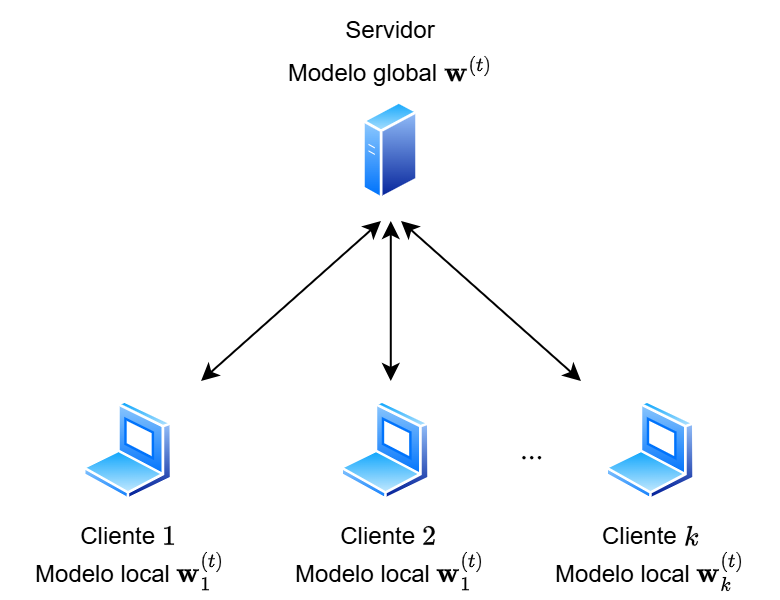
\includegraphics[width=0.8\textwidth]{./images/image1.png}
\caption{\label{fig:figure1}Ciclo de comunicación en aprendizaje federado.}
\end{center}
\end{figure}


\subsection{Proceso de optimización federada}

El objetivo del FL se puede formalizar como la minimización de una función de pérdida global
definida como el promedio ponderado de las pérdidas locales de cada cliente
\cite{DBLP:journals/corr/abs-1908-07873}:

\begin{equation}
  \min_{\mathbf{w}} F(\mathbf{w}) = \sum_{k=1}^{K} \frac{n_k}{n} F_k(\mathbf{w}),
  \label{eq:fedobj}
\end{equation}

donde $F_k(\mathbf{w}) = \frac{1}{n_k} \sum_{i \in \mathcal{D}_k} \ell(\mathbf{w}; x_i, y_i)$
es la función de pérdida local del cliente $k$ y $\ell$ es la función de pérdida por muestra
(por ejemplo, entropía cruzada para clasificación). En el caso ideal en que los datos de todos
los clientes siguen la misma distribución —condición IID—, el gradiente local $\nabla F_k
(\mathbf{w})$ es un estimado insesgado del gradiente global $\nabla F(\mathbf{w})$, y el
SGD distribuido converge a las mismas cotas que el SGD centralizado
\cite{li2020convergencefedavgnoniiddata}.

En la práctica, sin embargo, los datos federados raramente satisfacen la condición IID. Cuando
$\nabla F_k(\mathbf{w}) \neq \nabla F(\mathbf{w})$ para algún cliente $k$, los múltiples
pasos de SGD local producen una secuencia de parámetros que se aleja del óptimo global en la
dirección del óptimo local de $F_k$ \cite{DBLP:journals/corr/abs-1910-06378}. Al promediar
los parámetros locales al final de cada ronda, el modelo global resultante puede encontrarse
en una región de alta pérdida para todos los participantes, degradando la calidad del modelo
y ralentizando la convergencia. Este fenómeno, conocido como \textit{client drift}, es el
objeto de estudio central de la presente investigación y se formaliza en detalle en la
Sección~\ref{sec:clientdrift}.

\subsection{Desafíos del aprendizaje federado}

El FL introduce un conjunto de desafíos técnicos que no existen o se manifiestan con menor
severidad en el aprendizaje centralizado \cite{DBLP:journals/corr/abs-1912-04977,
DBLP:journals/corr/abs-1908-07873}. En el contexto de esta investigación, el más relevante es
la \textit{heterogeneidad estadística}: la distribución de datos entre clientes —tanto en
etiquetas como en características— difiere de forma sistemática, introduciendo un sesgo en el
gradiente local que el algoritmo de agregación debe compensar para preservar la convergencia
global. Esta dimensión se desarrolla en detalle en la Sección~\ref{sec:heterogeneidad}.

Un segundo desafío es la \textit{heterogeneidad del sistema}: los clientes presentan capacidades
computacionales y de memoria heterogéneas, velocidades de comunicación variables y posibles
caídas o desconexiones durante el entrenamiento \cite{DBLP:journals/corr/abs-1908-07873}. En
escenarios \textit{cross-device}, este factor puede dominar el rendimiento del sistema; en el
escenario \textit{cross-silo} de esta investigación, se controla manteniendo todos los clientes
activos en cada ronda con hiperparámetros de entrenamiento idénticos.

La \textit{privacidad y seguridad} constituye el tercer desafío estructural del FL
\cite{DBLP:journals/corr/abs-1912-04977}. Aunque los datos locales no se transmiten
directamente, las actualizaciones de parámetros pueden filtrar información sobre los datos de
entrenamiento mediante ataques de inversión de gradiente o inferencia de membresía
\cite{DBLP:journals/corr/abs-1807-00459}. Si bien la presente investigación no aborda
mecanismos de privacidad diferencial ni agregación segura, la motivación del FL en el
dominio médico descansa precisamente sobre esta restricción.

Finalmente, la \textit{eficiencia de comunicación} es un desafío práctico significativo: en cada
ronda de comunicación se transmiten todos los parámetros del modelo, cuyo tamaño puede superar
los cientos de megabytes para modelos modernos de visión \cite{mahmud2026survey}. Las cuatro
arquitecturas estudiadas en esta investigación se seleccionaron, entre otros criterios, por operar
a escalas de parámetros comparables y manejables ($\sim$5--8M parámetros), lo que hace que el
costo de comunicación sea equivalente entre familias y no constituya una variable de confusión.

% ============================================================
% 2.2 HETEROGENEIDAD ESTADÍSTICA Y CLIENT DRIFT
% ============================================================
\section{Heterogeneidad Estadística y Client Drift}
\label{sec:heterogeneidad}

\subsection{Datos IID y non-IID en aprendizaje federado}

En el aprendizaje automático estándar se asume que las muestras de entrenamiento son generadas
de forma independiente e idénticamente distribuida (IID) a partir de una distribución global
$P(X, Y)$ \cite{seo2025understanding}. En el contexto federado, esta condición implica que
cada cliente $k$ posee un subconjunto $\mathcal{D}_k$ muestreado de esa misma distribución
global, de modo que la distribución marginal de etiquetas y características es homogénea entre
participantes: $P_k(X, Y) \approx P(X, Y)$ para todo $k$.

En la práctica, los conjuntos de datos federados reales son no-IID (\textit{non-Independent and
Identically Distributed}): la distribución local $P_k(X, Y)$ varía entre clientes debido a
diferencias en las poblaciones atendidas, los protocolos de adquisición, los equipos utilizados
o los criterios de etiquetado \cite{g2024noniiddatafederatedlearning, seo2025understanding}.
Esta heterogeneidad tiene consecuencias directas sobre el proceso de optimización: si
$P_k(X, Y) \neq P_j(X, Y)$ para $k \neq j$, entonces $\nabla F_k(\mathbf{w}) \neq
\nabla F_j(\mathbf{w})$, y el gradiente promediado $\sum_k \frac{n_k}{n} \nabla F_k(\mathbf{w})$
puede apuntar en una dirección significativamente diferente al gradiente del óptimo global
$\nabla F(\mathbf{w})$ \cite{li2020convergencefedavgnoniiddata}. Li et al.\
\cite{li2020convergencefedavgnoniiddata} demostraron formalmente que, bajo condiciones non-IID,
FedAvg puede divergir o converger a un punto subóptimo distante del mínimo centralizado, con
una brecha de rendimiento que crece con el número de épocas locales $E$ y con el grado de
heterogeneidad entre los datos de los clientes.

\subsection{Taxonomía de la heterogeneidad}
\label{subsec:taxonomia}

Jiménez G. et al.\ \cite{g2024noniiddatafederatedlearning} proponen una taxonomía exhaustiva
de las formas en que los datos federados pueden diferir entre clientes. Las categorías
principales son:

\textbf{Sesgo de etiquetas} (\textit{label skew}): la distribución marginal de etiquetas
$P_k(Y)$ difiere entre clientes, mientras que la distribución condicional de características
dado la etiqueta $P_k(X \mid Y)$ puede ser homogénea. Es la forma más estudiada de
heterogeneidad y la que produce los efectos más severos sobre la convergencia
\cite{jimenez2503thorough}. En el contexto clínico, este sesgo es omnipresente: un hospital
especializado en oncología neurológica tendrá una proporción de tumores cerebrales muy
superior a la de un centro de atención primaria.

\textbf{Sesgo de características} (\textit{feature skew} o \textit{covariate shift}):
la distribución de entrada $P_k(X)$ varía entre clientes manteniendo constante la distribución
condicional $P_k(Y \mid X)$. Puede originarse en diferencias de equipamiento —distintos tipos
de escáneres MRI con protocolos de adquisición heterogéneos— o en variabilidad de iluminación,
resolución o preprocesamiento \cite{g2024noniiddatafederatedlearning}.

\textbf{Sesgo de cantidad} (\textit{quantity skew}): los clientes poseen volúmenes de datos
muy dispares, independientemente de la distribución de clases. Este desequilibrio afecta el
peso relativo de cada cliente en la agregación ponderada por $n_k / n$ y puede amplificar el
efecto del sesgo de etiquetas en los clientes con menos datos
\cite{g2024noniiddatafederatedlearning}.

\textbf{Heterogeneidad temporal}: la distribución de datos de un cliente varía a lo largo
del tiempo (\textit{concept drift}), lo que introduce inestabilidad adicional en el modelo
global \cite{DBLP:journals/corr/abs-1912-04977}.

La presente investigación opera exclusivamente sobre sesgo de etiquetas, controlado mediante
el parámetro de concentración $\alpha$ de la distribución de Dirichlet. Jiménez-Gutiérrez et al.\
\cite{jimenez2503thorough} han demostrado empíricamente que el sesgo de etiquetas produce
caídas de precisión de entre 10 y 40 puntos porcentuales sobre la línea base centralizada,
mientras que los sesgos de cantidad y características resultan prácticamente inocuos para
las arquitecturas estudiadas, lo que justifica la elección de este tipo de heterogeneidad
como variable experimental principal.

\subsection{Partición de Dirichlet para non-IID}

La distribución de Dirichlet $\text{Dir}(\alpha)$ es el mecanismo estándar para generar
particiones de datos con sesgo de etiquetas controlado en experimentos de FL
\cite{g2024noniiddatafederatedlearning, seo2025understanding}. Para un problema de
clasificación con $C$ clases y $K$ clientes, la partición se genera asignando a cada
cliente $k$ una proporción $\mathbf{q}_k = (q_{k,1}, \ldots, q_{k,C})$ muestreada de
$\text{Dir}(\alpha \cdot \mathbf{1}_C)$, donde $q_{k,c}$ es la fracción de muestras de la
clase $c$ asignadas al cliente $k$, satisfaciendo $\sum_k q_{k,c} = 1$ para toda clase $c$.

\sloppy El parámetro de concentración $\alpha > 0$ controla el grado de heterogeneidad: cuando
$\alpha \to 0$, cada cliente recibe datos de una única clase (heterogeneidad máxima); cuando
$\alpha \to \infty$, la partición converge a una distribución uniforme de clases (condición
IID) \cite{g2024noniiddatafederatedlearning}. La presente investigación emplea
$\alpha \in \{1000.0, 1.0, 0.3, 0.1, 0.03\}$, que cubren los regímenes de alta, media y baja heterogeneidad
respectivamente. A modo de referencia, Jiménez-Gutiérrez et al.\
\cite{jimenez2503thorough} reportan que los efectos críticos de degradación comienzan
a manifestarse de forma consistente para $\alpha \leq 0.5$ en las arquitecturas evaluadas.


\begin{figure} 
\begin{center}
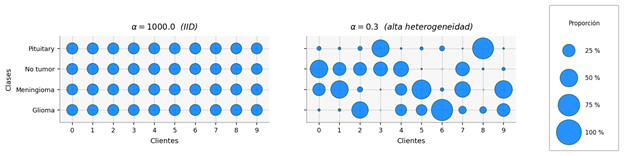
\includegraphics[width=\textwidth]{./images/image2.png}
\caption{\label{fig:figure2}Distribución de etiquetas por cliente bajo distintos valores de $\alpha$ — Brain Tumor MRI ($K=10$, semilla 42).}
\end{center}
\end{figure}

\subsection{Client drift: definición y mecanismo}
\label{sec:clientdrift}

El \textit{client drift} se define como la divergencia entre los parámetros del modelo de un
cliente al final de su entrenamiento local y el modelo global al inicio de esa misma ronda de
comunicación \cite{DBLP:journals/corr/abs-1910-06378}. Formalmente, dado que en la ronda $t$
el cliente $k$ recibe el modelo global $\mathbf{w}^{(t)}$ y realiza $E$ épocas de SGD local,
obteniendo $\mathbf{w}_k^{(t)}$, el vector de deriva del cliente $k$ se define como:

\begin{equation}
  \boldsymbol{\delta}_k^{(t)} = \mathbf{w}_k^{(t)} - \mathbf{w}^{(t)},
  \label{eq:drift}
\end{equation}

denominado en la literatura como \textit{pseudo-gradiente} \cite{DBLP:journals/corr/abs-1910-06378}.
El cliente drift es, por tanto, el efecto acumulado de múltiples pasos de SGD en la dirección
del óptimo local $\mathbf{w}_k^*$ en lugar del óptimo global $\mathbf{w}^*$.

El mecanismo causal del drift opera en tres niveles. En primer lugar, bajo condiciones non-IID,
el gradiente local $\nabla F_k(\mathbf{w})$ es un estimado sesgado del gradiente global
$\nabla F(\mathbf{w})$: existe una diferencia sistemática $\nabla F_k(\mathbf{w}) -
\nabla F(\mathbf{w}) \neq \mathbf{0}$ que depende de cuán diferente es $P_k(X,Y)$ respecto
a $P(X,Y)$ \cite{DBLP:journals/corr/abs-1910-06378}. En segundo lugar, este sesgo se amplifica
con cada paso adicional de SGD local: después de $E$ épocas, el modelo local se ha alejado de
$\mathbf{w}^{(t)}$ en la dirección del gradiente sesgado, acumulando una deriva proporcional
a $E$ y a la tasa de aprendizaje $\eta$ \cite{li2020convergencefedavgnoniiddata}. En tercer
lugar, al agregar los pseudo-gradientes $\boldsymbol{\delta}_k^{(t)}$ de múltiples clientes con
distribuciones distintas, el modelo global $\mathbf{w}^{(t+1)} = \mathbf{w}^{(t)} +
\sum_k \frac{n_k}{n} \boldsymbol{\delta}_k^{(t)}$ puede converger hacia un punto que minimiza
un promedio de funciones con óptimos en direcciones contradictorias, resultando en un modelo
subóptimo para todos los participantes \cite{DBLP:journals/corr/abs-1910-06378}.

Una observación fundamental para la presente investigación es que el drift no se distribuye
uniformemente entre las capas del modelo: trabajos como los de Son et al.\
\cite{son2022comparisons} han demostrado empíricamente que las capas de clasificación y de
normalización exhiben drift de mayor magnitud que las capas de extracción de características de
bajo nivel, y que esta distribución varía entre arquitecturas. Es precisamente esta estructura
interna del drift la que esta investigación busca caracterizar.




\begin{figure}[ht]
\centering
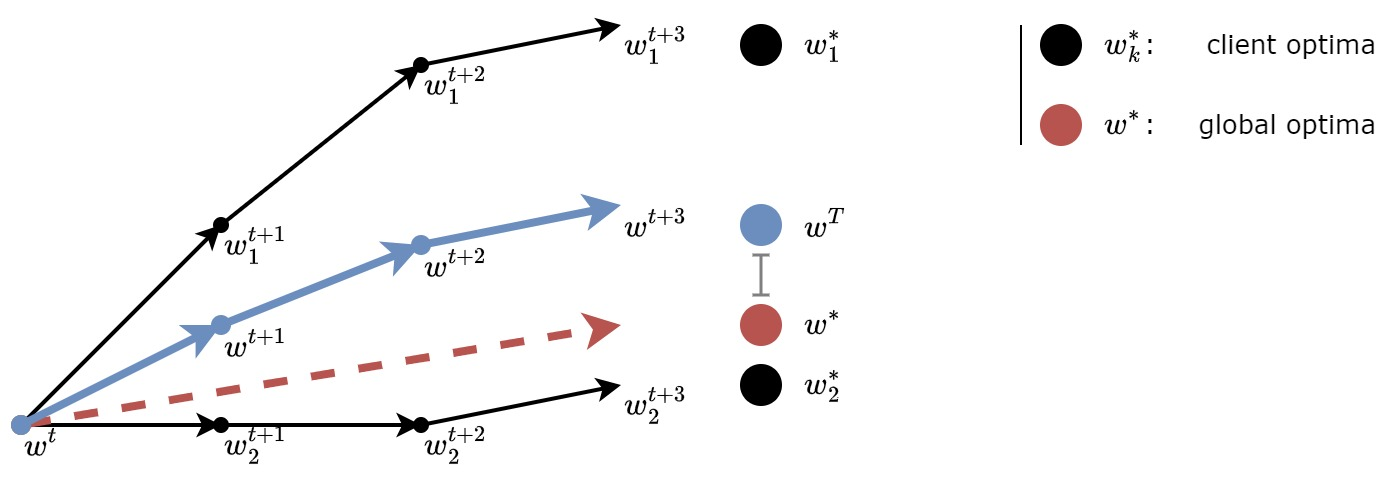
\includegraphics[width=\textwidth]{./images/image3.png}
\caption{Mecanismo del client drift en el espacio de parámetros.}
\label{fig:figure3}

\vspace{0.2cm}
\small Fuente: Obtenido de Le et al. (2024) \cite {le2024exploring}.
\end{figure}

\subsection{Impacto del drift sobre la convergencia}

Li et al.\ \cite{li2020convergencefedavgnoniiddata} demostraron que la cota de convergencia de
FedAvg bajo condiciones non-IID incluye un término adicional proporcional a la \textit{gradient
diversity}, definida como la discrepancia esperada entre los gradientes locales y el gradiente
global:

\begin{equation}
  \Gamma = F^* - \sum_{k=1}^{K} \frac{n_k}{n} F_k^*,
  \label{eq:diversity}
\end{equation}

donde $F^* = \min_{\mathbf{w}} F(\mathbf{w})$ es el óptimo global y $F_k^*$ es el óptimo
local del cliente $k$. Cuando los datos son IID, $\Gamma = 0$ y la cota de convergencia se
reduce a la del SGD centralizado. Bajo non-IID, $\Gamma > 0$ y actúa como un sesgo permanente
que no desaparece con el aumento del número de rondas de comunicación $T$
\cite{li2020convergencefedavgnoniiddata}. Este resultado teórico establece que la magnitud del drift, y por tanto de la degradación del rendimiento, depende directamente del grado de
heterogeneidad de los datos entre clientes, cuantificado en esta investigación mediante el
parámetro $\alpha$ de la distribución de Dirichlet.

Desde la perspectiva empírica, Karimireddy et al.\ \cite{DBLP:journals/corr/abs-1910-06378}
mostraron que FedAvg puede exhibir inestabilidad de convergencia incluso con tasas de
aprendizaje moderadas bajo alta heterogeneidad ($\alpha \to 0$), y que el número óptimo de
épocas locales $E$ decrece con el grado de no-IID. Esta dinámica es relevante para interpretar
los perfiles de drift registrados en el Capítulo de Análisis: una mayor oscilación de la curva
de accuracy a lo largo de las rondas es un indicador indirecto de un alto nivel de drift
acumulado.

% ============================================================
% 2.3 ALGORITMOS DE OPTIMIZACIÓN FEDERADA
% ============================================================
\section{Algoritmos de Optimización Federada}

\subsection{FedAvg}

El algoritmo FedAvg (\textit{Federated Averaging}), propuesto por McMahan et al.\
\cite{DBLP:journals/corr/McMahanMRA16}, constituye el método de referencia del aprendizaje
federado moderno. Su procedimiento es el siguiente: en cada ronda de comunicación $t$, el
servidor selecciona un subconjunto de $m$ clientes (o la totalidad de ellos en escenarios
\textit{cross-silo}), les envía el modelo global actual $\mathbf{w}^{(t)}$, cada cliente
realiza $E$ épocas de SGD local con tasa de aprendizaje $\eta$ sobre su conjunto de datos
$\mathcal{D}_k$, y el servidor agrega los modelos resultantes mediante un promedio ponderado
por tamaño de dataset:

\begin{equation}
  \mathbf{w}^{(t+1)} = \sum_{k=1}^{K} \frac{n_k}{n} \mathbf{w}_k^{(t)}.
  \label{eq:fedavg}
\end{equation}

La simplicidad algorítmica de FedAvg es su principal virtud: no requiere comunicación adicional
entre clientes, no introduce hiperparámetros dependientes de la arquitectura y se implementa
con cambios mínimos sobre cualquier bucle de entrenamiento estándar. Sin embargo, como se
mostró en la sección anterior, el promedio de parámetros locales entrenados sobre datos
heterogéneos puede producir un modelo global subóptimo \cite{li2020convergencefedavgnoniiddata}.
En esta investigación, FedAvg se emplea como algoritmo de referencia para caracterizar el
perfil de drift sin la intervención de mecanismos de corrección.

\subsection{FedProx}

\sloppy FedProx \cite{DBLP:journals/corr/abs-1812-06127}, propuesto por Sahu et al., extiende FedAvg
añadiendo un término de regularización proximal a la función de pérdida local de cada cliente:

\begin{equation}
  h_k(\mathbf{w}; \mathbf{w}^{(t)}) = F_k(\mathbf{w}) + \frac{\mu}{2}
  \|\mathbf{w} - \mathbf{w}^{(t)}\|^2,
  \label{eq:fedprox}
\end{equation}

donde $\mu \geq 0$ es el hiperparámetro de regularización proximal. El término
$\frac{\mu}{2}\|\mathbf{w} - \mathbf{w}^{(t)}\|^2$ penaliza el alejamiento del modelo
local respecto al modelo global recibido al inicio de la ronda, actuando como una restricción
suave que limita la magnitud del drift $\|\boldsymbol{\delta}_k^{(t)}\|$. Cuando $\mu = 0$,
FedProx se reduce a FedAvg. Al aumentar $\mu$, el modelo local se mantiene más cercano al
modelo global, lo que reduce el drift a costa de introducir un sesgo de regularización que
puede ralentizar la convergencia cuando los datos locales contienen información específica
valiosa \cite{DBLP:journals/corr/abs-1812-06127}.

Sahu et al.\ \cite{DBLP:journals/corr/abs-1812-06127} demostraron que FedProx converge bajo
condiciones de heterogeneidad estadística y de sistema donde FedAvg puede divergir, y que el
término proximal produce una mejora en la estabilidad del modelo global particularmente visible
bajo alta heterogeneidad. En esta investigación, FedProx se emplea con el objetivo de
evaluar si la reducción del drift producida por la regularización proximal interactúa de forma
diferente con las cuatro familias arquitectónicas, o si su efecto es homogéneo entre ellas.

\subsection{SCAFFOLD}

SCAFFOLD (\textit{Stochastic Controlled Averaging for Federated Learning}),
propuesto por Karimireddy et al.\ \cite{DBLP:journals/corr/abs-1910-06378}, introduce la
formalización más rigurosa del client drift al tiempo que propone su corrección mediante
variables de control de varianza. Cada cliente $k$ mantiene una variable de control
$\mathbf{c}_k$ que estima el gradiente local esperado, y el servidor mantiene $\mathbf{c}$
como estimado del gradiente global. La actualización de SGD local corregida por SCAFFOLD es:

\begin{equation}
  \mathbf{w}_k \leftarrow \mathbf{w}_k - \eta \left( \nabla F_k(\mathbf{w}_k)
  - \mathbf{c}_k + \mathbf{c} \right),
  \label{eq:scaffold}
\end{equation}

donde el término $-\mathbf{c}_k + \mathbf{c}$ actúa como una corrección de varianza que
compensa la diferencia entre el gradiente local y el global. Al final de cada ronda, las
variables de control se actualizan utilizando la diferencia entre las posiciones de los
parámetros antes y después del entrenamiento local. Karimireddy et al.\
\cite{DBLP:journals/corr/abs-1910-06378} demostraron que SCAFFOLD converge bajo condiciones
non-IID independientemente del número de épocas locales $E$ —propiedad que FedAvg no satisface
para $E > 1$ en escenarios heterogéneos.

SCAFFOLD no se emplea directamente como algoritmo experimental en esta investigación, pero su
marco teórico es central: la noción de pseudo-gradiente $\boldsymbol{\delta}_k^{(t)}$ definida
en la ecuación \eqref{eq:drift} proviene de este trabajo, y la corrección de varianza de
SCAFFOLD puede interpretarse como la operación inversa a la acumulación de drift. Comprender
SCAFFOLD es, por tanto, una condición necesaria para interpretar con precisión las métricas de
drift registradas en los experimentos.

% ============================================================
% 2.4 ARQUITECTURAS DE VISIÓN POR COMPUTADORA
% ============================================================
\section{Arquitecturas de Visión por Computadora}

Las cuatro familias arquitectónicas estudiadas en esta investigación —redes neuronales
convolucionales (CNNs), Vision Transformers (ViTs), State-Space Models (SSMs) y Vision Graph
Neural Networks (Vision GNNs)— procesan la información visual mediante mecanismos distintos. Estas diferencias estructurales se denominan \textit{sesgos
inductivos} (\textit{inductive biases}): suposiciones implícitas sobre la estructura de los
datos que determinan qué tipo de patrones puede aprender cada arquitectura de forma eficiente
\cite{xu2023fedconv}. Como se argumentará a lo largo de esta sección, los sesgos inductivos de
cada familia tienen implicaciones directas sobre su comportamiento bajo optimización federada
con datos heterogéneos, dado que determinan cómo los parámetros del modelo responden a las
distribuciones locales de cada cliente.


\begin{figure} 
\begin{center}
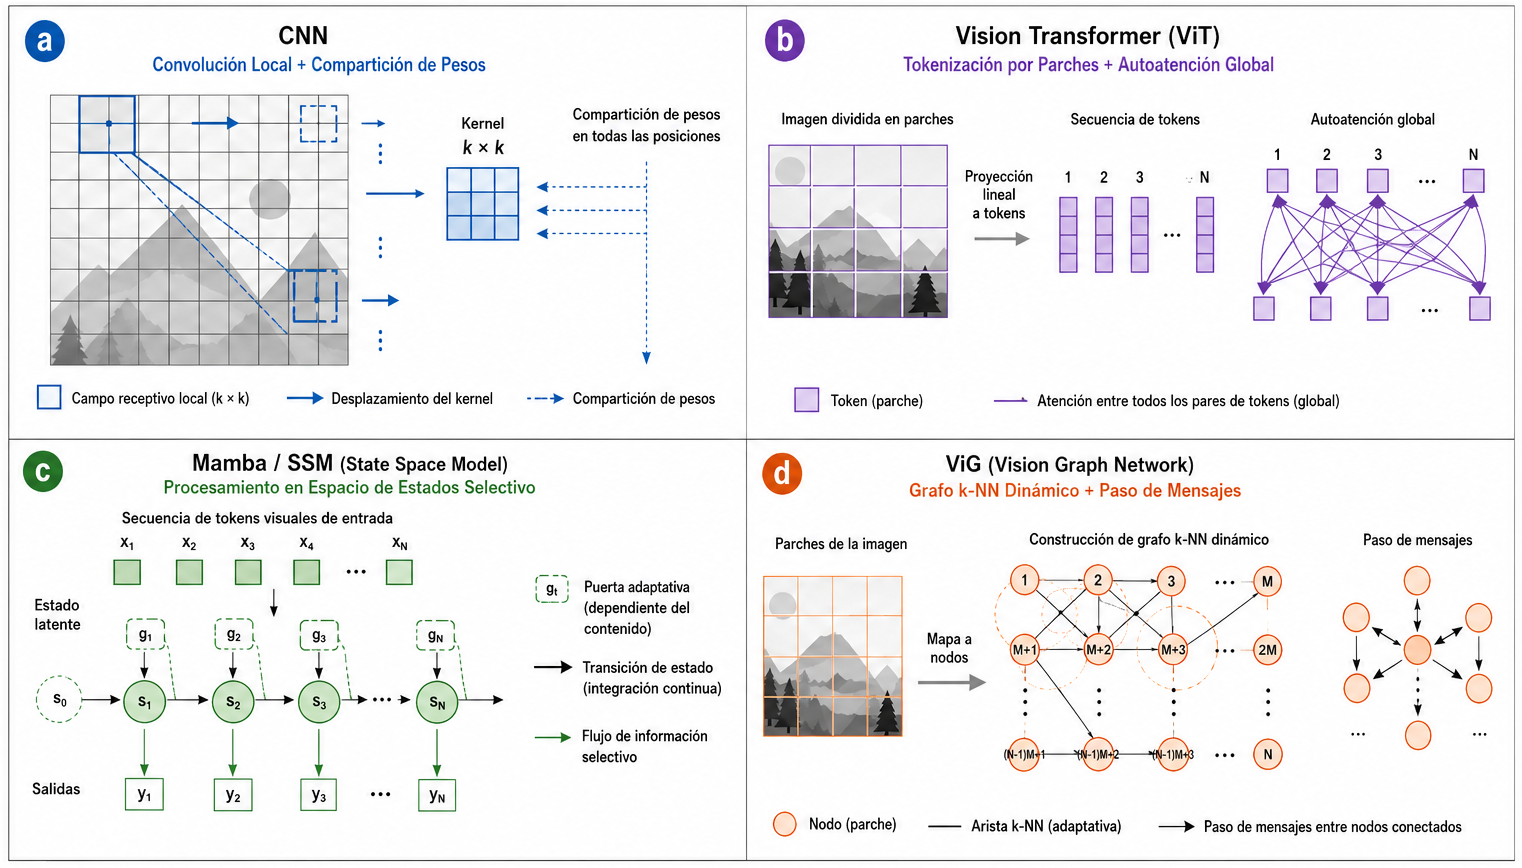
\includegraphics[width=\textwidth]{./images/image4.png}
\caption{\label{fig:figure4}Comparación de los sesgos inductivos en cuatro familias de arquitecturas de visión por computador.}
\end{center}
\end{figure}

\subsection{Redes Neuronales Convolucionales}

\subsubsection{Principios y sesgos inductivos}

Las redes neuronales convolucionales procesan la información visual mediante la operación de
convolución discreta \cite{heaton2018ian}. Dado
un mapa de activación de entrada $\mathbf{X} \in \mathbb{R}^{H \times W \times C_{in}}$, una
capa convolucional aplica un conjunto de filtros $\mathbf{F} \in \mathbb{R}^{k \times k \times
C_{in} \times C_{out}}$ de tamaño $k \times k$, donde cada filtro recorre la imagen de forma
deslizante produciendo un mapa de respuesta de dimensiones reducidas. El parámetro compartido
más importante es el filtro en sí: el mismo conjunto de pesos $\mathbf{F}$ se aplica en todas
las posiciones espaciales de la imagen (\textit{weight sharing}), lo que confiere a las CNNs
el sesgo inductivo de \textit{equivarianza traslacional}: si un patrón se desplaza en la imagen,
su representación se desplaza de forma correspondiente en el mapa de activación
\cite{xu2023fedconv}.

Los sesgos inductivos de la CNN son tres: (1) \textit{localidad espacial}, dado que cada
neurona de salida depende únicamente de una región $k \times k$ de la entrada;
(2) \textit{equivarianza traslacional}, consecuencia directa del weight sharing; y
(3) \textit{jerarquía de características}, donde las capas iniciales aprenden detectores de
bordes y texturas de bajo nivel, y las capas profundas combinan estos detectores para
representar objetos complejos \cite{pieri2023handlingdataheterogeneityarchitectural}.

En el contexto federado, la localidad espacial implica que los filtros convolucionales aprenden
patrones visuales locales que son altamente dependientes de las clases presentes en los datos de
entrenamiento de cada cliente. Bajo sesgo de etiquetas severo ($\alpha = 0.1$), los filtros de
distintos clientes pueden especializarse en detectar características propias de las clases
locales, dando lugar a representaciones locales incompatibles que producen un alto drift al ser
promediadas \cite{qu2022rethinking}.


\begin{figure}
\begin{center}
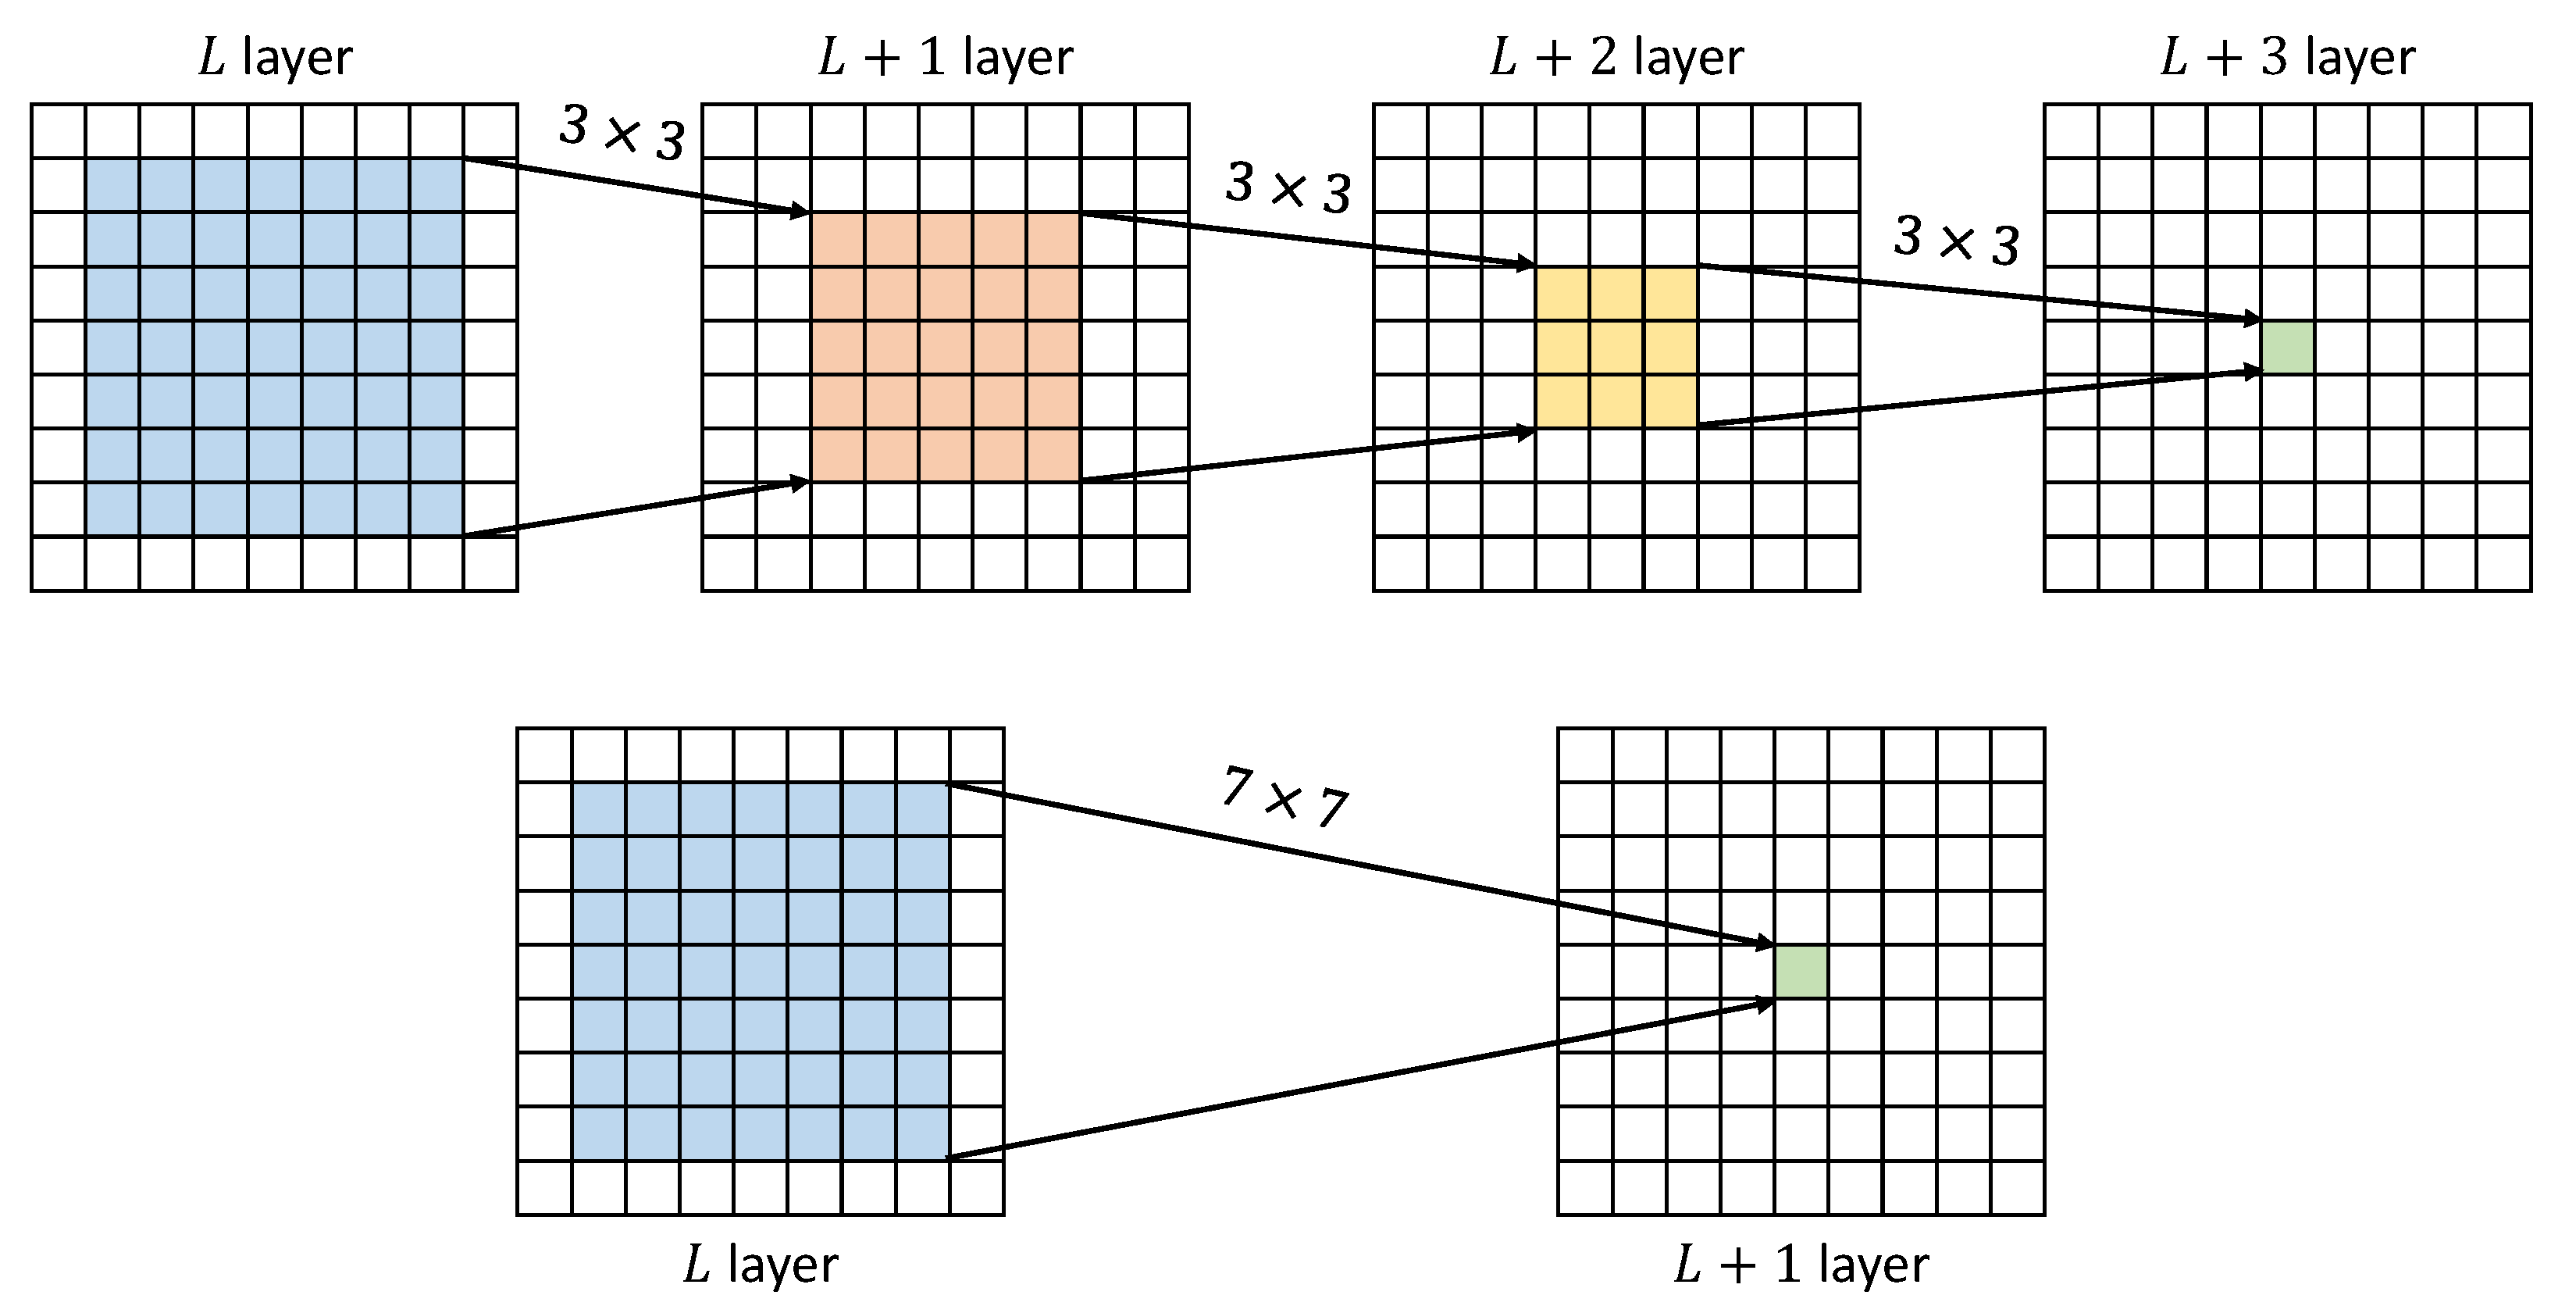
\includegraphics[width=\textwidth]{./images/image5.png}
\caption{\label{fig:figure5} Convolución discreta de un filtro \textit{$3\times3$} sobre un mapa de activación. Una pila de tres capas convolucionales de \textit{$3\times3$} tiene un campo receptivo efectivo de \textit{$7\times7$}.}

\vspace{0.2cm}
\small Fuente: Obtenido de Dong et al. (2023) \cite{app13063403}.

\end{center}
\end{figure}

\subsubsection{EfficientNet-B1 y la familia EfficientNet}

EfficientNet \cite{DBLP:journals/corr/abs-1905-11946} es una familia de
redes neuronales convolucionales diseñada mediante escalado compuesto (\textit{compound
scaling}): en lugar de escalar únicamente la profundidad, la anchura o la resolución de la red
de forma independiente, EfficientNet escala las tres dimensiones simultáneamente siguiendo
coeficientes determinados por búsqueda de arquitectura neural (NAS). EfficientNet-B1 es una de las variantes de menor tamaño de la familia, con aproximadamente 5.3 millones de parámetros y una
resolución de entrada estándar de $224 \times 224$ píxeles.

El bloque constructivo de EfficientNet es el \textit{MBConv} (\textit{Mobile Inverted
Bottleneck Convolution}), que combina una convolución puntual de expansión, una convolución
\textit{depthwise} separable y un módulo de \textit{Squeeze-and-Excitation} (SE) que recalibra
los mapas de canales mediante atención de canal global. Esta combinación hace a EfficientNet
computacionalmente eficiente al reducir el número de parámetros respecto a las redes totalmente
densas, mientras que el módulo SE introduce una forma limitada de contexto global dentro de
cada bloque, aunque sin llegar a la atención global de los ViTs
\cite{pieri2023handlingdataheterogeneityarchitectural}.

EfficientNet-B1 es el representante CNN elegido en esta investigación por tres razones: (1) su
escala de parámetros es comparable con ViT-Tiny y Vim-Tiny, eliminando el tamaño del modelo
como variable de confusión; (2) ha sido ampliamente utilizado en benchmarks de imagenología
médica, incluida la clasificación de tumores cerebrales \cite{chenfederated}; y (3) su
dependencia de Batch Normalization lo convierte en el candidato natural para la ablación de
normalización descrita en la Sección \ref{subsec:normalizacion}.

\begin{figure} 
\begin{center}
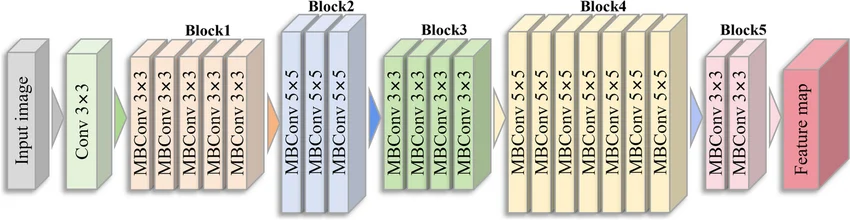
\includegraphics[width=\textwidth]{./images/image6.png}
\caption{\label{fig:figure6}Arquitectura EfficientNet-B1.}
\vspace{0.2cm}
\small Fuente: Obtenido de Dai et al. (2025) \cite {dai2025image}.

\end{center}
\end{figure}

\subsubsection{Batch Normalization y su interacción con FL}

Batch Normalization (BN) \cite{DBLP:journals/corr/IoffeS15} es una técnica de normalización que estandariza las activaciones de cada capa
usando las estadísticas del mini-batch actual. Para una activación $x$ en el mini-batch
$\mathcal{B} = \{x_1, \ldots, x_m\}$:

\begin{equation}
  \text{BN}(x) = \gamma \cdot \frac{x - \hat{\mu}_{\mathcal{B}}}
  {\sqrt{\hat{\sigma}^2_{\mathcal{B}} + \varepsilon}} + \beta,
  \label{eq:bn}
\end{equation}

donde $\hat{\mu}_{\mathcal{B}} = \frac{1}{m}\sum_{i=1}^m x_i$ y
$\hat{\sigma}^2_{\mathcal{B}} = \frac{1}{m}\sum_{i=1}^m (x_i - \hat{\mu}_{\mathcal{B}})^2$
son la media y varianza del mini-batch, y $\gamma$, $\beta$ son parámetros aprendibles de
escala y desplazamiento. Adicionalmente, BN mantiene estadísticas móviles (\textit{running
mean} y \textit{running variance}) que se actualizan durante el entrenamiento y se utilizan
durante la inferencia.

En el entorno federado con datos non-IID, BN introduce una vulnerabilidad específica que ha
sido formalizada por Wang et al.\ \cite{wang2023batch}: dado que cada cliente computa
$\hat{\mu}_{\mathcal{B}}^{(k)}$ y $\left(\hat{\sigma}^{2}_{\mathcal{B}}\right)^{(k)}$ sobre mini-batches
muestreados de su distribución local $P_k(X)$, las estadísticas resultantes son estimados
sesgados de las estadísticas globales $\mu$ y $\sigma^2$ de la distribución global $P(X)$.
Este sesgo tiene dos consecuencias sobre el modelo global producido por FedAvg. Primero, un
\textit{desajuste en el forward pass}: cuando los parámetros aprendibles $\gamma$, $\beta$
son promediados entre clientes, el modelo global hereda una normalización calibrada para
estadísticas locales inconsistentes entre sí, corrompiendo las representaciones intermedias
para todas las muestras \cite{wang2023batch}. Segundo, un \textit{desajuste en el backward
pass}: los gradientes respecto a $\gamma$ y $\beta$ se calculan usando las estadísticas locales
de cada cliente, de modo que las actualizaciones de estos parámetros apuntan en direcciones
distintas para clientes con distribuciones heterogéneas, amplificando el drift en las capas
de normalización \cite{du2022rethinking}.

Wang et al.\ \cite{wang2023batch} demostraron analíticamente que este sesgo de gradiente
inducido por BN es proporcional a la discrepancia entre las estadísticas locales y globales,
y que su magnitud crece con el grado de heterogeneidad. Du et al.\ \cite{du2022rethinking}
confirmaron empíricamente que la sustitución de BN por estrategias de normalización
independientes del batch —Layer Normalization o Group Normalization— reduce de forma
consistente la degradación del rendimiento bajo condiciones non-IID.

\subsection{Vision Transformers}

\subsubsection{Mecanismo de autoatención y tokenización}

Los Vision Transformers (ViT) \cite{DBLP:journals/corr/abs-2010-11929} adaptan la arquitectura
Transformer, originalmente desarrollada para procesamiento de lenguaje natural, al dominio de
la visión por computadora mediante un proceso de tokenización de la imagen. Dada una imagen
de entrada $\mathbf{I} \in \mathbb{R}^{H \times W \times C}$, se divide en $N = \frac{HW}{P^2}$
parches no solapados de tamaño $P \times P$ píxeles. Cada parche se aplana y se proyecta
linealmente a un vector de dimensión $d$, produciendo una secuencia de tokens
$\mathbf{Z} = [\mathbf{z}_1, \ldots, \mathbf{z}_N] \in \mathbb{R}^{N \times d}$. Se añade
un token de clasificación \texttt{[CLS]} y codificaciones posicionales para preservar
información espacial.

El bloque central de los ViTs es el mecanismo de \textit{Multi-Head Self-Attention} (MHSA).
Para un conjunto de tokens $\mathbf{Z}$, las matrices de consulta $\mathbf{Q}$, clave
$\mathbf{K}$ y valor $\mathbf{V}$ se obtienen mediante proyecciones lineales:

\begin{equation}
  \text{Attention}(\mathbf{Q}, \mathbf{K}, \mathbf{V}) =
  \text{softmax}\!\left(\frac{\mathbf{Q}\mathbf{K}^\top}{\sqrt{d_k}}\right)\mathbf{V},
  \label{eq:attention}
\end{equation}

donde $d_k$ es la dimensión de las cabezas de atención. La propiedad clave de este mecanismo
es que cada token puede atender simultáneamente a todos los demás tokens de la secuencia,
estableciendo dependencias globales desde la primera capa sin ninguna restricción de localidad
espacial \cite{qu2022rethinking}. Este sesgo inductivo —la capacidad de capturar contexto
global— contrasta fundamentalmente con la localidad de las CNNs.

En el contexto federado, la ausencia de dependencia de estadísticas de mini-batch hace que el
mecanismo de atención no sufra el desajuste de normalización identificado para las CNNs con BN.
La variabilidad entre clientes se manifiesta en cambio en los patrones de atención aprendidos
—las matrices $\mathbf{Q}$, $\mathbf{K}$, $\mathbf{V}$— que pueden especializarse en las
relaciones entre regiones de imagen propias de las clases locales de cada cliente
\cite{qu2022rethinking, pieri2023handlingdataheterogeneityarchitectural}.



\begin{figure}[ht]
\centering
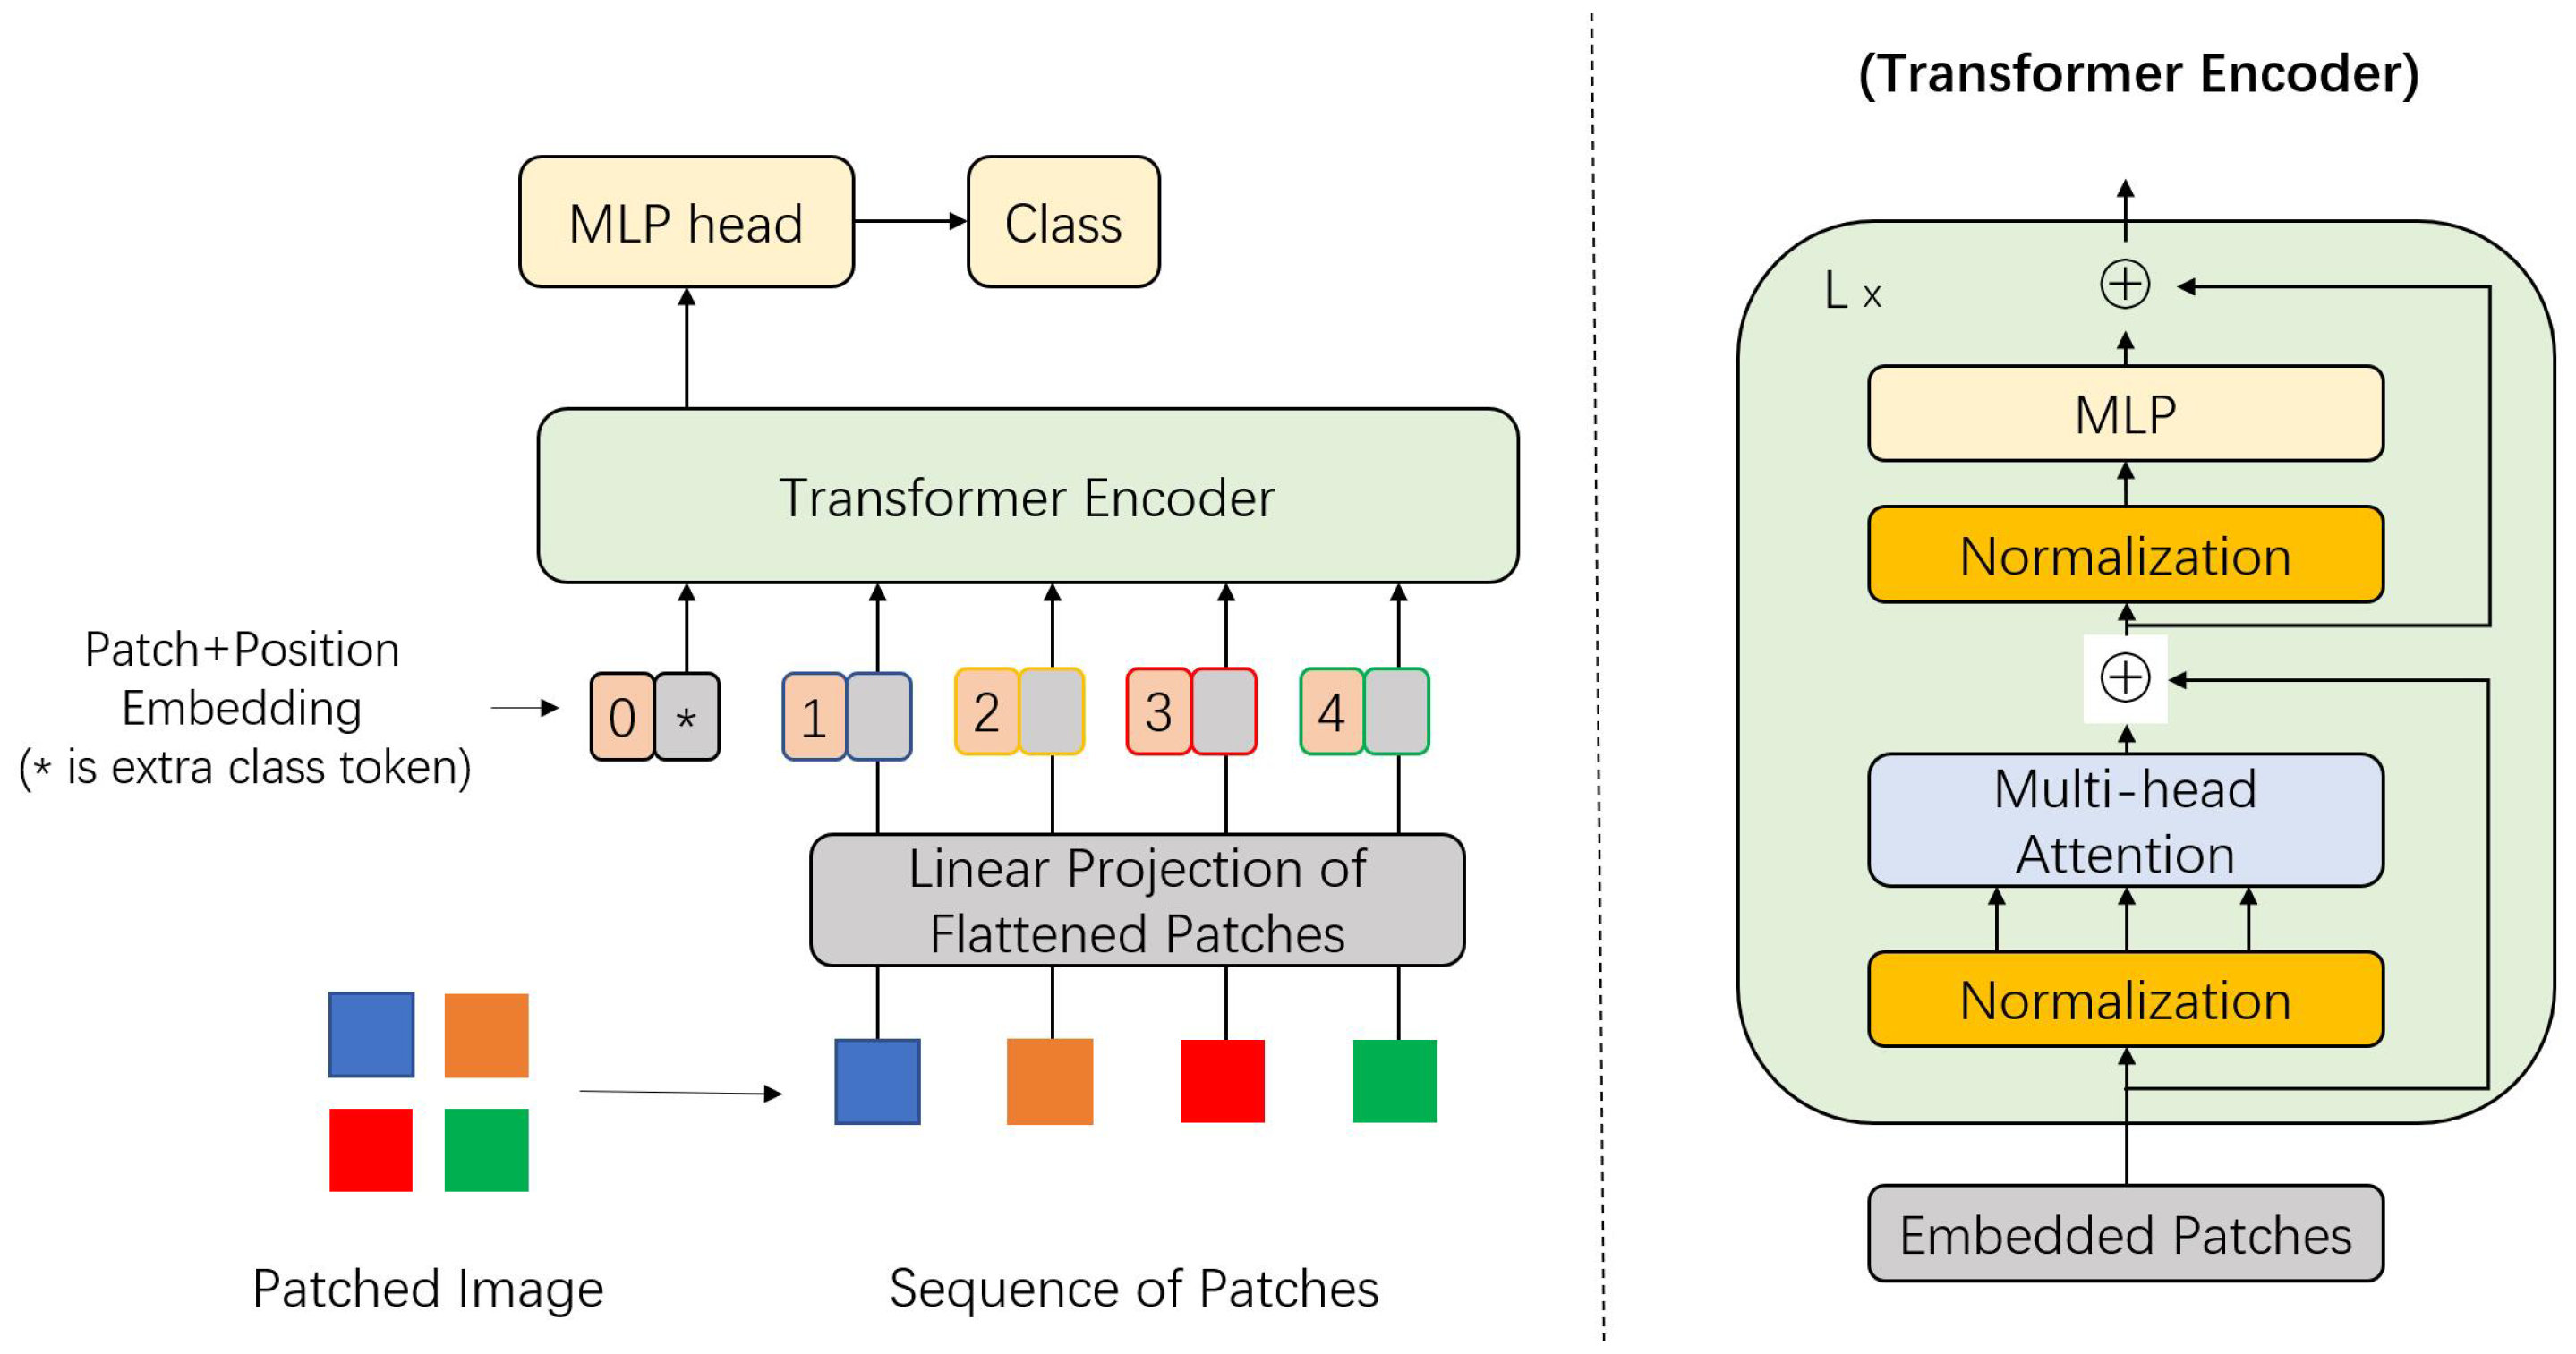
\includegraphics[width=\textwidth]{./images/image7.png}
\caption{Arquitectura de Vision Transformer.}
\label{fig:figure7}

\vspace{0.2cm}
\small Fuente: Obtenido de Wang et al. (2025) \cite{wang2025vision}.
\end{figure}



\subsubsection{ViT-Tiny}

El modelo empleado en esta investigación es \texttt{vit\_tiny\_patch16\_224}, cargado mediante
la librería \texttt{timm}. Esta variante usa parches de $16 \times 16$ píxeles sobre imágenes
de $224 \times 224$, generando $N = 196$ tokens. La dimensión de embedding es $d = 192$, con 3
cabezas de atención y 12 bloques Transformer, resultando en aproximadamente 5.7 millones de
parámetros. LayerNorm \cite{ba2016layernormalization} se aplica de forma nativa antes de cada bloque de atención y antes
de cada bloque MLP (\textit{pre-norm}), en contraste con la arquitectura original de Transformer
que usaba \textit{post-norm}.

ViT-Tiny se selecciona como representante de la familia ViT por ser la variante de menor costo
computacional con rendimiento competitivo en clasificación de imágenes, y por su escala de
parámetros comparable con EfficientNet-B1 y Vim-Tiny, lo que garantiza una comparación
arquitectónica justa. Su uso de LayerNorm nativo lo ubica, desde la perspectiva de la
normalización, en el extremo opuesto a EfficientNet-B1 con BN, siendo el modelo de referencia
para la estabilidad federada esperada según la literatura
\cite{wang2023batch, casella2023experimentingnormalizationlayersfederated}.


\begin{figure}[ht]
\centering
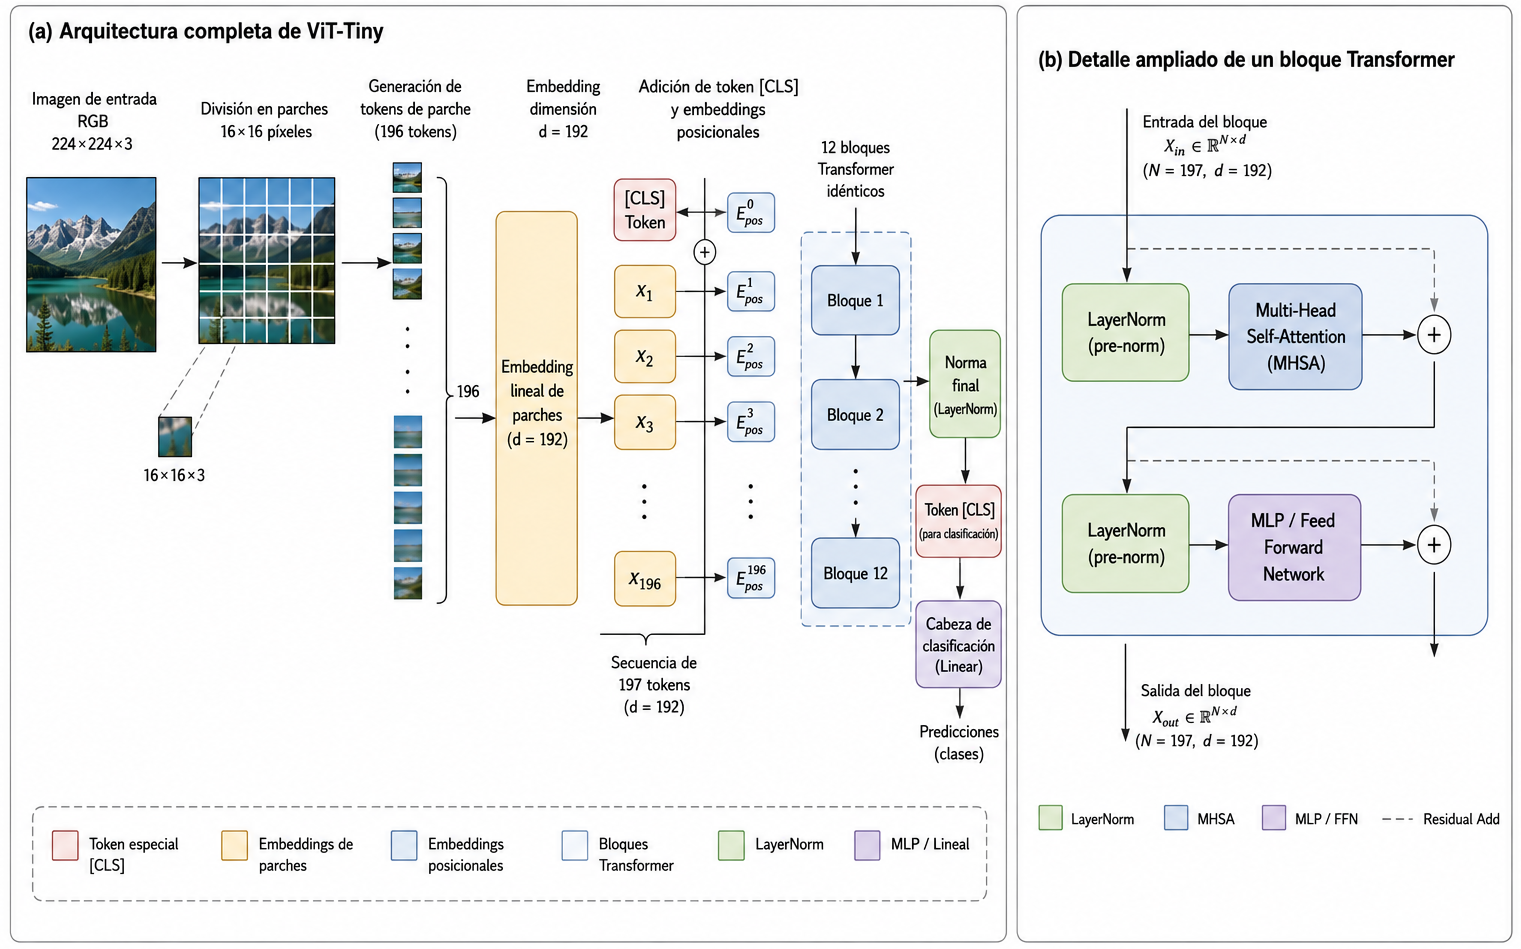
\includegraphics[width=\textwidth]{./images/image8.png}
\caption{Estructura completa de ViT-Tiny (\texttt{vit\_tiny\_patch16\_224})}
\label{fig:figure8}


\end{figure}


\subsubsection{Layer Normalization}

Layer Normalization (LN) \cite{ba2016layernormalization}
normaliza las activaciones a lo largo de la dimensión de características de una única muestra,
en lugar de a lo largo de la dimensión del batch como hace BN. Para una activación
$\mathbf{x} \in \mathbb{R}^d$ de una muestra individual:

\begin{equation}
  \text{LN}(\mathbf{x}) = \gamma \cdot
  \frac{\mathbf{x} - \mu_{\mathbf{x}}}{\sqrt{\sigma^2_{\mathbf{x}} + \varepsilon}} + \beta,
  \label{eq:ln}
\end{equation}

donde $\mu_{\mathbf{x}} = \frac{1}{d}\sum_{i=1}^d x_i$ y $\sigma^2_{\mathbf{x}} =
\frac{1}{d}\sum_{i=1}^d (x_i - \mu_{\mathbf{x}})^2$ son la media y varianza calculadas sobre
las $d$ características de esa muestra. La propiedad fundamental de LN en el contexto federado
es que las estadísticas $\mu_{\mathbf{x}}$ y $\sigma^2_{\mathbf{x}}$ se calculan de forma
independiente para cada muestra, sin acumular información sobre la distribución del batch ni
mantener estadísticas móviles \cite{casella2023experimentingnormalizationlayersfederated}. En
consecuencia, los parámetros $\gamma$ y $\beta$ de LN aprendidos por diferentes clientes son
comparables entre sí y sus promedios son funcionalmente coherentes, eliminando el desajuste de
normalización que introducía BN \cite{du2022rethinking}.

\subsection{State Space Models: Vision Mamba}

\subsubsection{State Space Models y la ecuación de espacio de estados}

Los modelos de espacio de estados (SSM, \textit{State Space Models}) son sistemas dinámicos
lineales que modelan la relación entre una señal de entrada $x(t)$ y una señal de salida $y(t)$
a través de un estado latente $\mathbf{h}(t) \in \mathbb{R}^N$ \cite{qu2024survey}. El SSM
continuo se define mediante las ecuaciones:

\begin{equation}
  \mathbf{h}'(t) = \mathbf{A}\,\mathbf{h}(t) + \mathbf{B}\,x(t), \qquad
  y(t) = \mathbf{C}\,\mathbf{h}(t) + D\,x(t),
  \label{eq:ssm_cont}
\end{equation}

donde $\mathbf{A} \in \mathbb{R}^{N \times N}$ es la matriz de transición de estado,
$\mathbf{B} \in \mathbb{R}^{N \times 1}$ es la matriz de entrada, $\mathbf{C} \in
\mathbb{R}^{1 \times N}$ es la matriz de salida y $D$ es el término de salto directo.
Para su implementación en modelos de aprendizaje profundo, el SSM se discretiza mediante el
método \textit{Zero-Order Hold} (ZOH) con paso de tiempo $\Delta$, obteniendo:

\begin{equation}
  \bar{\mathbf{A}} = e^{\Delta\mathbf{A}}, \quad
  \bar{\mathbf{B}} = (\Delta\mathbf{A})^{-1}(e^{\Delta\mathbf{A}} - \mathbf{I})\,\Delta\mathbf{B},
  \label{eq:ssm_disc}
\end{equation}

con la recurrencia discreta $\mathbf{h}_t = \bar{\mathbf{A}}\,\mathbf{h}_{t-1} +
\bar{\mathbf{B}}\,x_t$, $y_t = \mathbf{C}\,\mathbf{h}_t + D\,x_t$ \cite{zhu2024vision}.
Una propiedad computacional relevante es que los SSMs con matrices $\mathbf{A}$, $\mathbf{B}$,
$\mathbf{C}$ fijas pueden evaluarse tanto mediante la recurrencia (complejidad lineal en
longitud de secuencia $L$, $\mathcal{O}(L)$) como mediante una convolución global (complejidad
$\mathcal{O}(L \log L)$), ambas más eficientes que la autoatención cuadrática
$\mathcal{O}(L^2)$ de los ViTs \cite{qu2024survey}.

El modelo Mamba introduce los SSMs selectivos (S6): las matrices $\mathbf{B}$, $\mathbf{C}$ y
el paso de tiempo $\Delta$ pasan a ser funciones del input en lugar de ser parámetros fijos,
lo que confiere al modelo la capacidad de filtrar selectivamente qué información propagar en
el estado latente dependiendo del contenido de la secuencia \cite{zhu2024vision}. Esta
\textit{selectividad dependiente del contenido} diferencia fundamentalmente a Mamba de los
SSMs lineales clásicos y lo aproxima, en términos de capacidad expresiva, a los ViTs, aunque
con un mecanismo de integración de la información cualitativamente distinto.

\begin{figure}[ht]
\centering
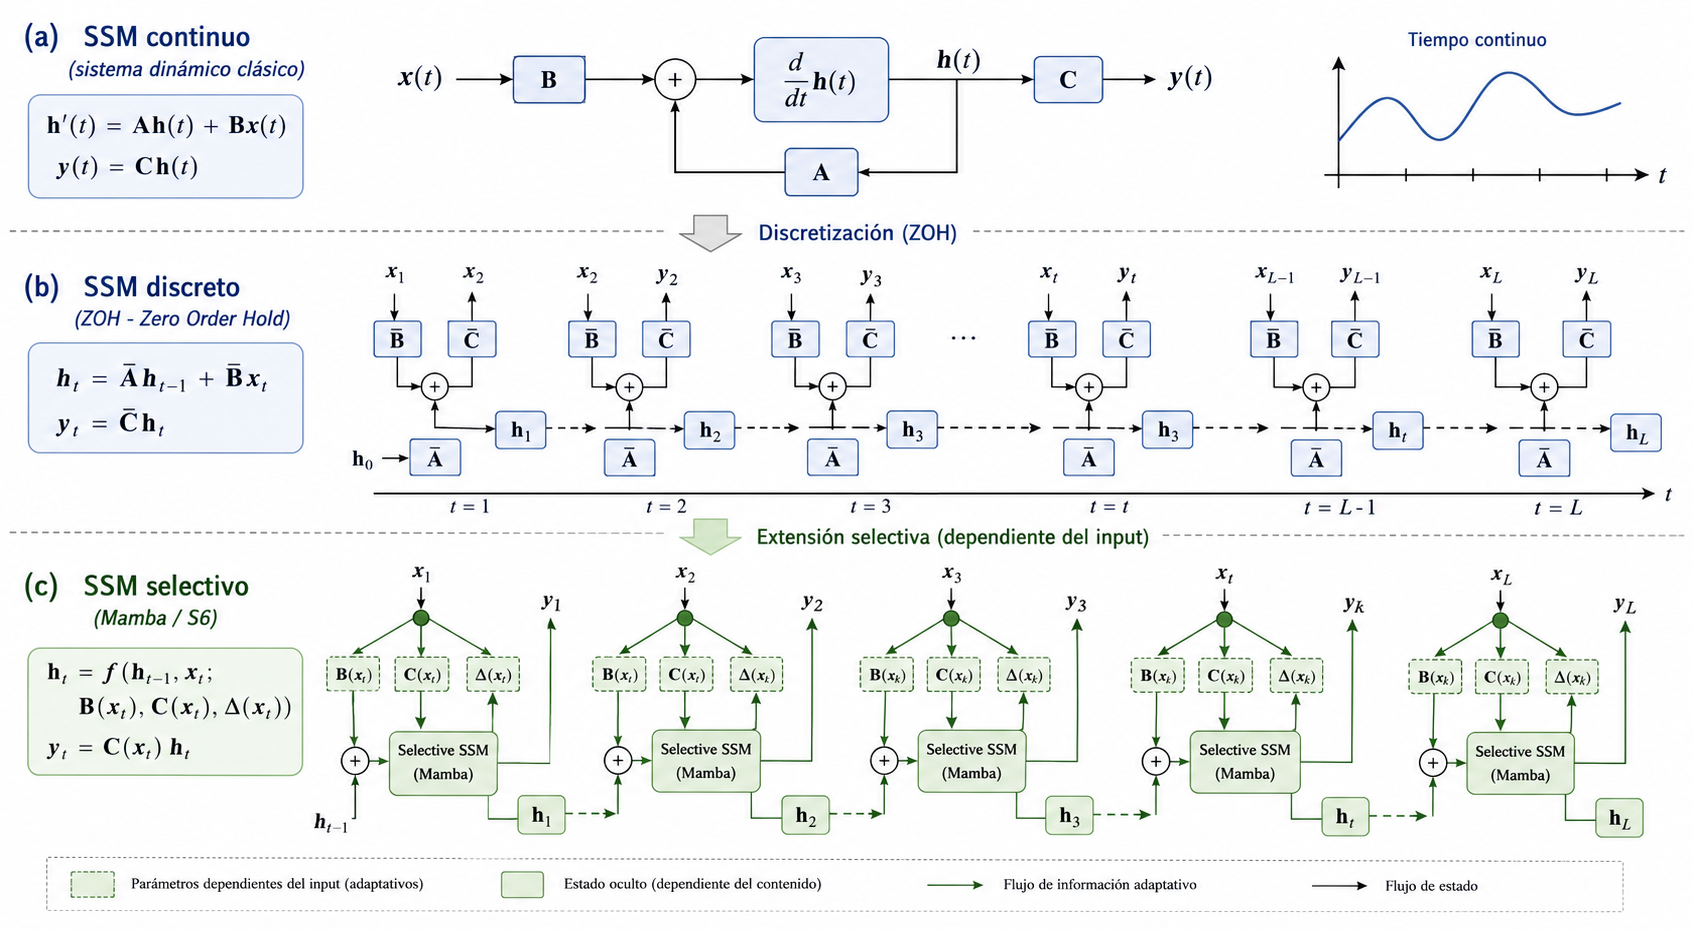
\includegraphics[width=\textwidth]{./images/image9.png}
\caption{Evolución del SSM — lineal, discreto y selectivo (Mamba).}
\label{fig:figure9}
\end{figure}

\subsubsection{Vision Mamba (Vim-Tiny)}

Vision Mamba (Vim) \cite{zhu2024vision} adapta los SSMs selectivos al dominio de la visión
por computadora introduciendo un bloque SSM bidireccional sobre la secuencia de parches de
imagen. La imagen de entrada se tokeniza de la misma forma que en ViT, generando una secuencia
de $N$ tokens. Cada bloque Vim procesa la secuencia en dos direcciones —de izquierda a derecha
y de derecha a izquierda— y fusiona las salidas para producir representaciones bidireccionales,
capturando dependencias tanto causales como anti-causales en la secuencia espacial de parches.

Vim-Tiny, la variante utilizada en esta investigación, cuenta con aproximadamente 7 millones de
parámetros y emplea LayerNorm de forma nativa al inicio de cada bloque, lo que lo sitúa en la
misma categoría de normalización que ViT-Tiny desde la perspectiva de la estabilidad federada.
No obstante, su mecanismo de integración de la información es cualitativamente distinto al de
los ViTs: mientras que la autoatención establece dependencias globales simultáneas entre todos
los pares de tokens, el SSM integra la información mediante transiciones de estado secuenciales
cuya sensibilidad a cada token de entrada depende de la magnitud de $\Delta$ calculado a partir
de ese token \cite{zhu2024vision}. Bajo distribuciones de clases locales distintas entre
clientes, los parámetros SSM —especialmente las proyecciones para $\mathbf{B}$, $\mathbf{C}$ y
$\Delta$— pueden especializarse en secuencias locales representativas de las clases locales,
generando un perfil de drift potencialmente distinto al de ViT \cite{wu2024mamba}.

Desde la perspectiva del rendimiento en dominios médicos, Lai et al.\ \cite{lai2025advancing}
demostraron la competitividad de Vision Mamba en clasificación de tumores cerebrales mediante
\textit{transfer learning}, obteniendo resultados comparables a EfficientNet y ViT. Bansal et
al.\ \cite{bansal2024comprehensive} confirman esta competitividad en múltiples modalidades de
imagen médica. Sin embargo, el comportamiento de Vim-Tiny en el contexto del FL con datos
non-IID y su perfil de drift por capa permanecen sin caracterizar en la literatura existente.


\begin{figure}[ht]
\centering
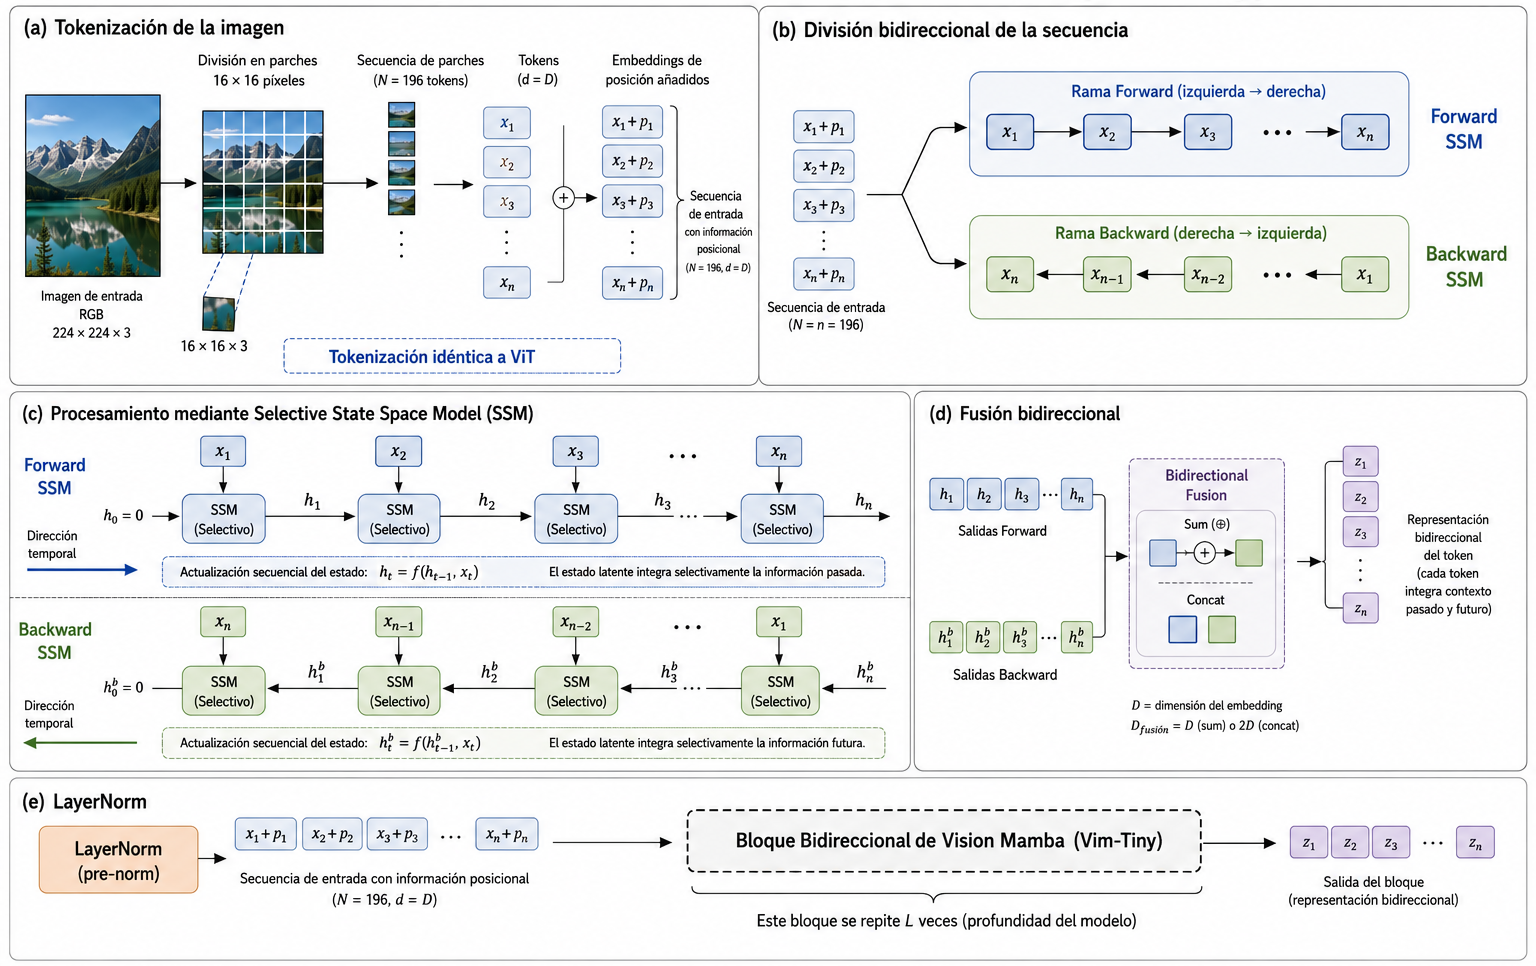
\includegraphics[width=\textwidth]{./images/image10.png}
\caption{Bloque bidireccional de Vision Mamba (Vim).}
\label{fig:figure10}


\end{figure}

\subsection{Vision Graph Neural Networks}

\subsubsection{Graph Neural Networks: propagación de mensajes}

Las redes neuronales en grafos (GNN, \textit{Graph Neural Networks}) son una clase de modelos
de aprendizaje profundo diseñados para operar sobre datos con estructura de grafo
\cite{Scarselli:2009ku}. Un grafo se define como $\mathcal{G} = (\mathcal{V}, \mathcal{E})$,
donde $\mathcal{V} = \{v_1, \ldots, v_n\}$ es el conjunto de nodos y $\mathcal{E} \subseteq
\mathcal{V} \times \mathcal{V}$ es el conjunto de aristas. Cada nodo $v$ posee una
representación vectorial $\mathbf{h}_v^{(l)} \in \mathbb{R}^d$ en la capa $l$, que se actualiza
mediante un proceso de \textit{propagación de mensajes} sobre el vecindario local
$\mathcal{N}(v)$ del nodo:

\begin{equation}
  \mathbf{h}_v^{(l+1)} = \text{UPDATE}\!\left(
    \mathbf{h}_v^{(l)},\;
    \text{AGGREGATE}\!\left(\left\{\mathbf{h}_u^{(l)} : u \in \mathcal{N}(v)\right\}\right)
  \right),
  \label{eq:mpnn}
\end{equation}

donde AGGREGATE es una función permutation-invariante —típicamente suma, media o máximo— y
UPDATE combina la representación actual del nodo con la información agregada de sus vecinos
\cite{Scarselli:2009ku}. El proceso se repite por $L$ capas, permitiendo que cada nodo integre
información de su vecindario de orden $L$.

La propiedad diferenciadora de las GNNs respecto a las CNNs y los ViTs es que la topología
de conectividad —quién es vecino de quién— puede ser dinámica y dependiente del contenido:
las aristas $\mathcal{E}$ no son una restricción estructural fija (como en las CNNs, donde el
vecindario es siempre el parche $k \times k$ adyacente) ni una conectividad completa (como en
los ViTs, donde todos los tokens se atienden mutuamente), sino que pueden construirse
dinámicamente a partir de medidas de similitud en el espacio de representaciones
\cite{senior2023graph, han2022vision}.


\begin{figure}[ht]
\centering
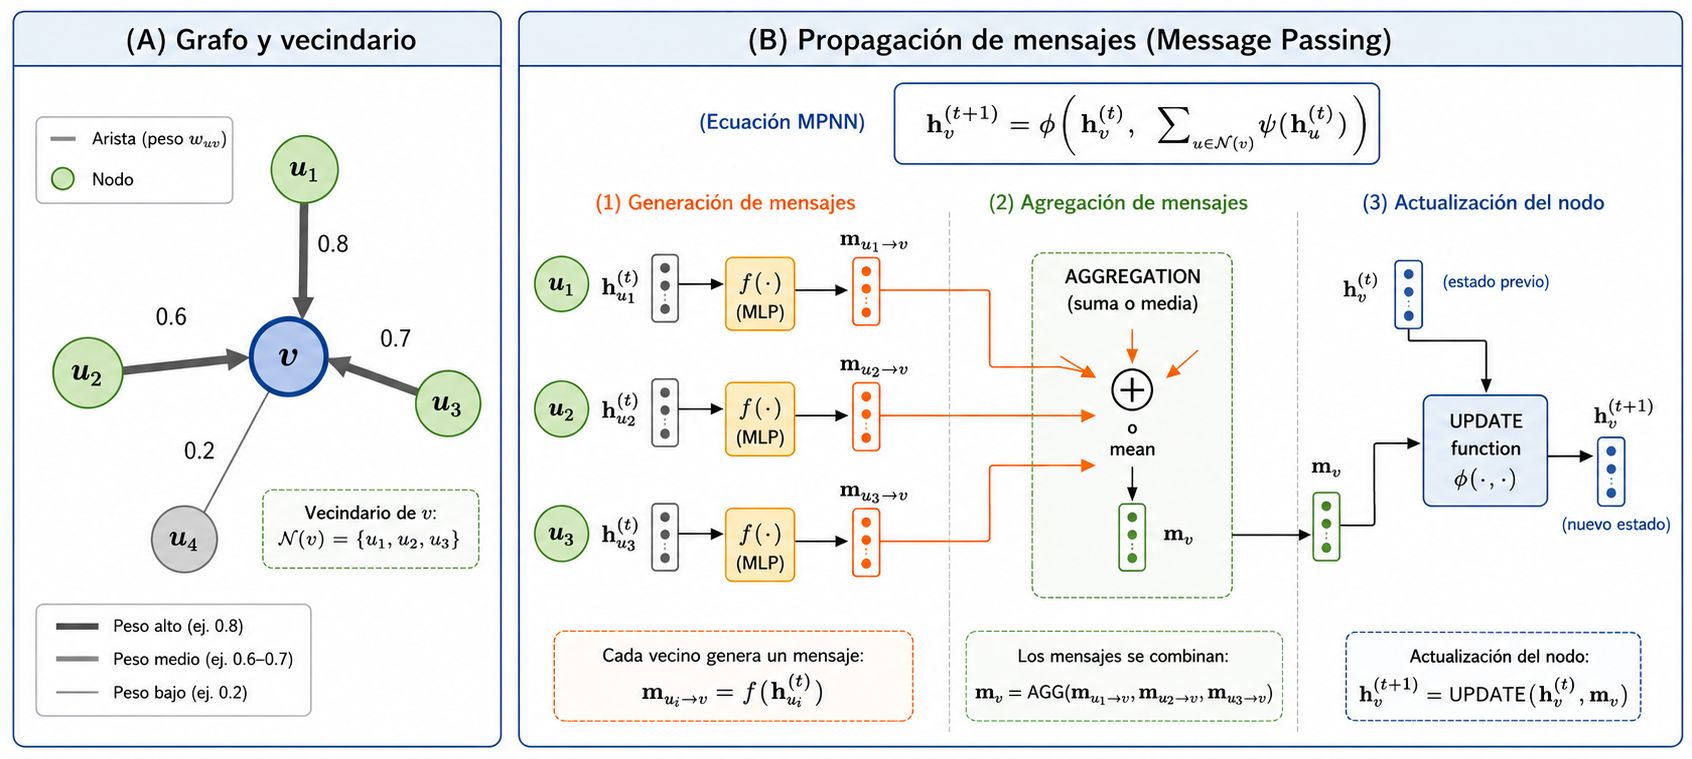
\includegraphics[width=\textwidth]{./images/image11.png}
\caption{Propagación de mensajes en una Graph Neural Network.}
\label{fig:figure11}


\end{figure}


\subsubsection{Vision GNN (ViG-Tiny)}

Han et al.\ \cite{han2022vision} introdujeron Vision GNN (ViG), la primera arquitectura de
visión pura basada en grafos diseñada para clasificación de imágenes a escala de ImageNet.
La arquitectura trata la imagen como un grafo dinámico: los nodos son parches de la imagen,
y las aristas se construyen mediante un grafo $k$-NN (\textit{k-Nearest Neighbors}) en el
espacio de representaciones aprendidas —los $k$ parches más similares en el espacio de
features se conectan mediante aristas dirigidas. Este grafo se reconstruye en cada bloque
a medida que las representaciones evolucionan durante el forward pass, haciendo que la
topología de conectividad sea adaptativa al contenido de la imagen \cite{han2022vision}.

El bloque central de ViG es el \textit{Grapher}, que implementa una operación GNN sobre el
grafo dinámico construido en ese bloque, seguido de un módulo FFN (\textit{Feed-Forward
Network}) análogo al de los ViTs:

\begin{equation}
  \mathbf{H}^{(l+1)} = \text{FFN}\!\left(\text{GNN}\!\left(\mathbf{H}^{(l)},
  \mathcal{G}^{(l)}\right)\right),
  \label{eq:vig_block}
\end{equation}

donde $\mathcal{G}^{(l)}$ es el grafo $k$-NN construido a partir de $\mathbf{H}^{(l)}$
\cite{han2022vision}. La variante ViG-Tiny cuenta con aproximadamente 8 millones de
parámetros y opera sobre imágenes de $224 \times 224$ píxeles, con resolución de tokens
comparable a ViT-Tiny.

El sesgo inductivo de ViG es cualitativamente distinto al de las otras tres familias: la
localidad de las CNNs es espacial y fija; la globalidad de los ViTs es completa y uniforme;
la secuencialidad de los SSMs es lineal y selectiva; la conectividad de ViG es dinámica y
basada en similitud de contenido. Bajo distribuciones de clases locales distintas, el grafo
$k$-NN construido por cada cliente tenderá a conectar parches visualmente similares según las
clases predominantes en sus datos locales, lo que puede introducir patrones de especialización
del Grapher cualitativamente distintos a los de los mecanismos de atención o SSM
\cite{liu2024federated}. La caracterización de este comportamiento en entornos federados
heterogéneos es una de las contribuciones originales de la presente investigación.

Han et al.\ \cite{han2022vision} reportaron resultados competitivos en ImageNet-1K, con ViG-Tiny
superando a DeiT-Tiny en precisión \textit{top-1}. La viabilidad de ViG en entornos federados
fue explorada por primera vez por Cui et al.\ \cite{cui2025fedvig} mediante FedVIG, aunque sin
análisis sistemático de heterogeneidad ni métricas de drift por capa. El presente trabajo
extiende esta línea al entorno experimental controlado de esta investigación.


\begin{figure}[ht]
\centering
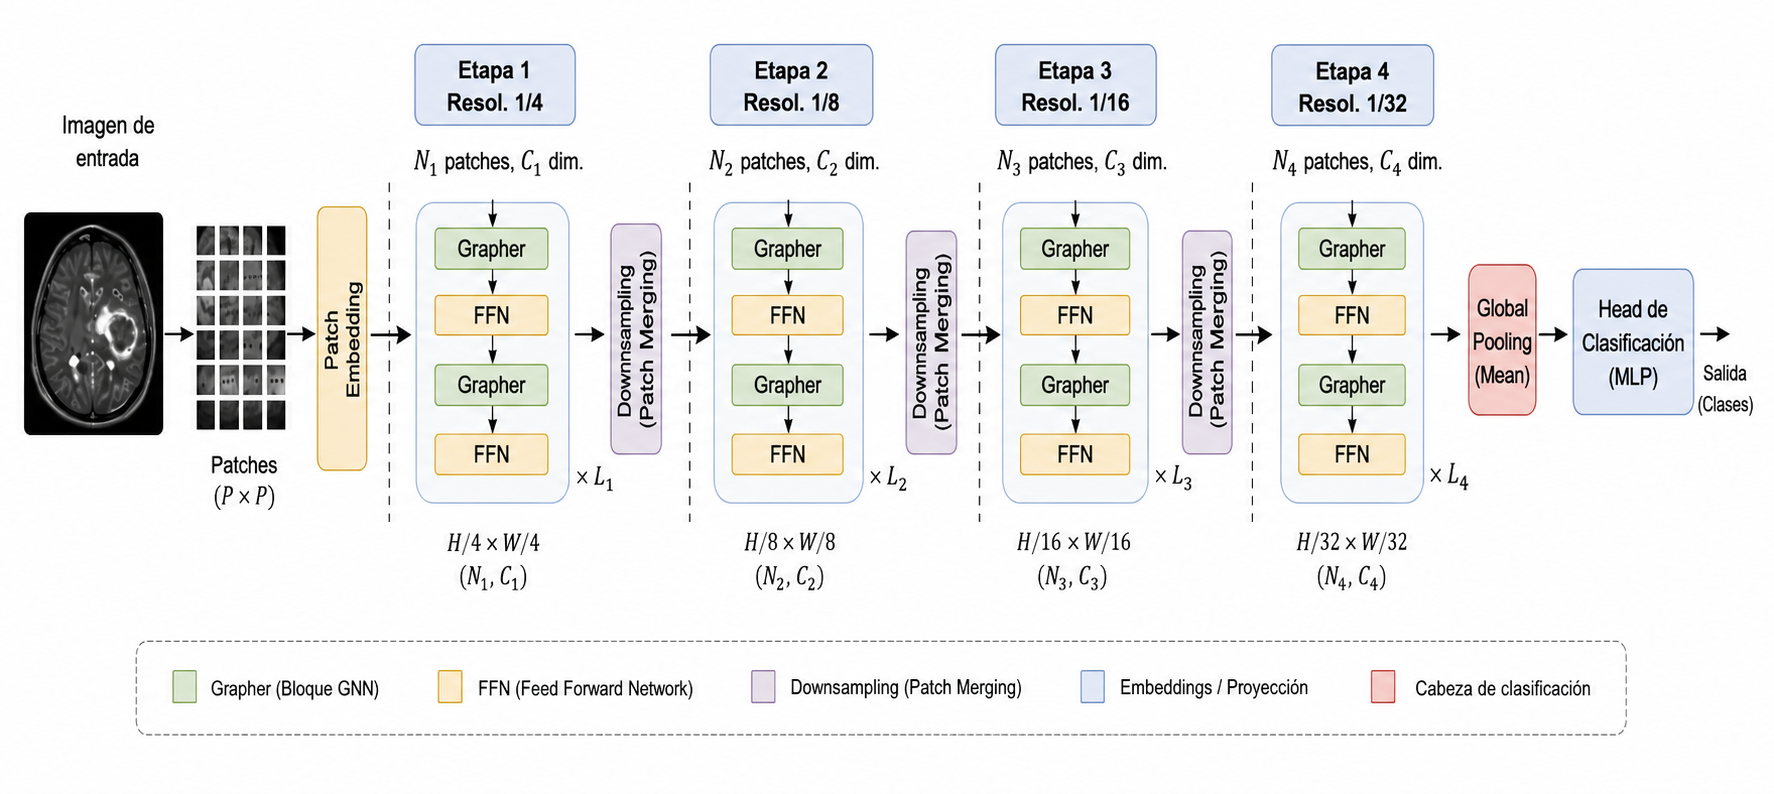
\includegraphics[width=\textwidth]{./images/image12.png}
\caption{Arquitectura de Arquitectura ViG-Tiny.}
\label{fig:figure12}


\end{figure}


\subsection{Estrategias de normalización y sus propiedades en FL}
\label{subsec:normalizacion}

Las distintas estrategias de normalización descritas en las secciones anteriores se diferencian
fundamentalmente por el subconjunto de dimensiones sobre el que calculan las estadísticas de
media y varianza. Esta diferencia determina directamente su estabilidad en entornos federados
con datos heterogéneos \cite{wang2023batch, du2022rethinking, casella2023experimentingnormalizationlayersfederated}.

\textbf{Batch Normalization} (BN) \cite{DBLP:journals/corr/IoffeS15}: normaliza
sobre la dimensión del batch y las dimensiones espaciales, manteniendo estadísticas separadas
por canal. Las estadísticas $\hat{\mu}_{\mathcal{B}}$ y $\hat{\sigma}^2_{\mathcal{B}}$ se
calculan sobre todas las muestras del mini-batch. En FL, estas estadísticas son locales al
cliente y no representan la distribución global, introduciendo el sesgo de gradiente descrito
en la Sección 2.4.1.3 \cite{wang2023batch}.

\textbf{Group Normalization} (GN) \cite{DBLP:journals/corr/abs-1803-08494}: propuesta por Wu
y He, divide los canales de activación en $G$ grupos y normaliza dentro de cada grupo de forma
independiente para cada muestra. Para una activación $\mathbf{x} \in \mathbb{R}^{C \times H
\times W}$, GN calcula:

\begin{equation}
  \mu_{k,g} = \frac{1}{|\mathcal{S}_{k,g}|}\sum_{i \in \mathcal{S}_{k,g}} x_i, \qquad
  \sigma^2_{k,g} = \frac{1}{|\mathcal{S}_{k,g}|}\sum_{i \in \mathcal{S}_{k,g}}
  (x_i - \mu_{k,g})^2,
  \label{eq:gn}
\end{equation}

donde $\mathcal{S}_{k,g}$ es el conjunto de índices del grupo $g$ para la muestra $k$, con
$C/G$ canales por grupo. GN con $G = 1$ es equivalente a Layer Normalization; GN con $G = C$
es equivalente a Instance Normalization. Dado que las estadísticas se calculan por muestra y
por grupo, GN es completamente independiente de la distribución del batch y, en consecuencia,
estable en entornos federados con datos heterogéneos \cite{DBLP:journals/corr/abs-1803-08494,
casella2023experimentingnormalizationlayersfederated}.

La motivación de la ablación de normalización de esta investigación se deriva directamente de
esta taxonomía: al sustituir la BN de EfficientNet-B1 por GN-32 (32 grupos) y por LN
(equivalente a GN-1), se obtienen dos variantes que
conservan exactamente el mismo sesgo inductivo convolucional pero eliminan la dependencia de estadísticas
de mini-batch. Si el
perfil de drift de estas variantes se aproxima al de ViT-Tiny y Vim-Tiny, se concluye que BN
es el factor dominante en la inestabilidad federada de las CNNs; si persisten diferencias
significativas, el sesgo inductivo convolucional tiene una contribución independiente
\cite{pieri2023handlingdataheterogeneityarchitectural, siomos2024architecture}.

% ============================================================
% 2.5 MÉTRICAS DE ANÁLISIS DEL CLIENT DRIFT
% ============================================================
\section{M\'etricas de An\'alisis del Client Drift}

Para caracterizar el client drift con la granularidad requerida por los objetivos de esta
investigación, se necesitan métricas que operen en tres niveles complementarios y no
redundantes: (1) la \textit{divergencia de parámetros}, que cuantifica cuánto se alejan los
pesos del modelo de cada cliente del modelo global en términos de magnitud; (2) la
\textit{alineación de gradientes}, que determina si las actualizaciones de distintos clientes
son constructivas o destructivas entre sí en términos de dirección; y (3) la
\textit{divergencia representacional funcional}, que evalúa si el drift paramétrico implica
o no una divergencia en las representaciones que el modelo aprende a generar. Las tres métricas
empleadas en esta investigación cubren uno de esos niveles cada una, y son complementarias:
sus combinaciones permiten diagnósticos que ninguna métrica individual puede proporcionar de
forma aislada.

\subsection{Divergencia de pesos por capa (\texorpdfstring{$L_2$}{L2} drift)}

La métrica más directa para cuantificar el client drift es la norma $L_2$ de la diferencia
entre los parámetros del modelo local de un cliente y los parámetros del modelo global,
calculada de forma separada para cada capa. Para el cliente $k$, la capa $\ell$ y la ronda de
comunicación $t$, la divergencia de pesos se define como:

\begin{equation}
  \text{drift}_k^{(\ell)}(t) = \left\| \mathbf{w}_k^{(\ell)}(t) -
  \mathbf{w}_{\text{global}}^{(\ell)}(t) \right\|_2,
  \label{eq:l2drift}
\end{equation}

donde $\mathbf{w}_k^{(\ell)}(t)$ son los parámetros de la capa $\ell$ del cliente $k$
inmediatamente antes de la agregación de la ronda $t$, y $\mathbf{w}_{\text{global}}^{(\ell)}(t)$
son los parámetros correspondientes del modelo global al inicio de esa misma ronda. Esta métrica
es la operacionalización directa del pseudo-gradiente definido en la ecuación \eqref{eq:drift},
calculada a nivel de capa en lugar de para el modelo completo \cite{son2022comparisons}.

La estratificación por tipo de capa es fundamental para la interpretabilidad de los resultados.
En esta investigación, los parámetros de cada arquitectura se clasifican en tres grupos
taxonómicos:

\begin{itemize}
  \item \textbf{norm}: capas de normalización (BN, GN o LN según la arquitectura y variante).
  \item \textbf{feature}: capas de extracción de características (bloques MBConv en
    EfficientNet, bloques de atención y MLP en ViT-Tiny, bloques SSM en Vim-Tiny, bloques
    Grapher en ViG-Tiny).
  \item \textbf{head}: la capa clasificadora final (proyección lineal sobre el vector de clase).
\end{itemize}

Son et al.\ \cite{son2022comparisons} establecieron empíricamente que las capas de
clasificación (\textit{head}) exhiben drift sistemáticamente mayor que las capas de extracción
de características de bajo nivel, y que las capas de normalización son las más sensibles a la
heterogeneidad cuando se usa BN. Esta taxonomía permite comparaciones significativas entre
familias arquitectónicas a pesar de que la noción de ``capa de características'' no es
directamente equiparable entre CNNs, ViTs, SSMs y GNNs \cite{son2022comparisons}.

\subsection{Alineación de gradientes entre clientes (similitud coseno)}

La norma $L_2$ del drift cuantifica la magnitud de la divergencia pero no informa sobre si las
actualizaciones de distintos clientes son compatibles entre sí. Dos clientes pueden presentar
alta magnitud de drift pero apuntar en la misma dirección (actualizaciones constructivas) o en
direcciones opuestas (actualizaciones destructivas para la agregación). Para distinguir estos
casos, se emplea la similitud coseno entre los pseudo-gradientes de pares de clientes,
calculada por capa.

Para los clientes $i$ y $j$, la capa $\ell$ y la ronda $t$, la similitud coseno se define como:

\begin{equation}
  \text{cos\_sim}_{i,j}^{(\ell)}(t) =
  \frac{\boldsymbol{\delta}_i^{(\ell)}(t) \cdot \boldsymbol{\delta}_j^{(\ell)}(t)}
  {\left\|\boldsymbol{\delta}_i^{(\ell)}(t)\right\|_2
   \left\|\boldsymbol{\delta}_j^{(\ell)}(t)\right\|_2},
  \label{eq:cossim}
\end{equation}

donde $\boldsymbol{\delta}_k^{(\ell)}(t) = \mathbf{w}_k^{(\ell)}(t) -
\mathbf{w}_{\text{global}}^{(\ell)}(t)$ es el pseudo-gradiente del cliente $k$ en la capa
$\ell$. El resultado toma valores en $[-1, 1]$: valores positivos indican que las
actualizaciones apuntan en la misma dirección general (refuerzo mutuo al promediar); valores
negativos indican que apuntan en direcciones opuestas (interferencia destructiva); el valor
cero indica ortogonalidad (sin interacción constructiva ni destructiva). El perfil de
alineación de gradientes de una arquitectura se obtiene promediando la ecuación \eqref{eq:cossim}
sobre todos los pares $(i, j)$ con $i < j$, reportando el resultado por tipo de capa y por
ronda de comunicación.

Esta métrica es complementaria al $L_2$ drift: una arquitectura puede exhibir bajo drift $L_2$
pero alta interferencia (pseudo-gradientes de pequeña magnitud pero orientaciones opuestas), o
alto drift $L_2$ pero buena alineación (grandes actualizaciones en direcciones consistentes).
La combinación de ambas métricas proporciona un diagnóstico más completo del comportamiento de
la optimización federada que cualquiera de las dos por separado \cite{son2022comparisons}.

\subsection{Centered Kernel Alignment (CKA)}

\subsubsection{Similitud de representaciones neurales}

Las métricas $L_2$ y coseno descritas anteriormente operan sobre los parámetros del modelo y
sus diferencias. Sin embargo, dos modelos con parámetros muy distintos pueden aprender
representaciones funcionalmente equivalentes, especialmente si sus espacios de parámetros son relacionados por transformaciones
ortogonales o de escala \cite{DBLP:journals/corr/abs-1905-00414}. Para evaluar si el drift
paramétrico implica una divergencia funcional en las representaciones aprendidas, se requiere
una métrica que opere directamente sobre las activaciones del modelo y que sea invariante a
transformaciones que no cambian la función computada.

El Centered Kernel Alignment (CKA) \cite{DBLP:journals/corr/abs-1905-00414}, propuesto por
Kornblith et al., satisface esta propiedad. Dadas las matrices de activaciones
$\mathbf{X} \in \mathbb{R}^{n \times p}$ e $\mathbf{Y} \in \mathbb{R}^{n \times q}$
obtenidas al evaluar dos modelos (o el mismo modelo en dos momentos distintos) sobre el mismo
conjunto de $n$ muestras, CKA mide si las relaciones de similitud entre pares de muestras son
consistentes entre las dos representaciones.

\subsubsection{Definición formal del CKA lineal}

El CKA lineal se basa en el estimador de Hilbert-Schmidt Independence Criterion (HSIC) para
matrices de Gram centradas. Las matrices de Gram son:

\begin{equation}
  \mathbf{K} = \mathbf{X}\mathbf{X}^\top \in \mathbb{R}^{n \times n}, \qquad
  \mathbf{L} = \mathbf{Y}\mathbf{Y}^\top \in \mathbb{R}^{n \times n},
  \label{eq:gram}
\end{equation}

y el estimador HSIC centrado es:

\begin{equation}
  \widehat{\text{HSIC}}(\mathbf{K}, \mathbf{L}) =
  \frac{1}{(n-1)^2} \operatorname{tr}(\mathbf{K}\mathbf{H}\mathbf{L}\mathbf{H}),
  \label{eq:hsic}
\end{equation}

donde $\mathbf{H} = \mathbf{I}_n - \frac{1}{n}\mathbf{1}\mathbf{1}^\top$ es la matriz de
centrado. El CKA lineal se define como:

\begin{equation}
  \text{CKA}(\mathbf{X}, \mathbf{Y}) =
  \frac{\widehat{\text{HSIC}}(\mathbf{K}, \mathbf{L})}
  {\sqrt{\widehat{\text{HSIC}}(\mathbf{K}, \mathbf{K})\,
         \widehat{\text{HSIC}}(\mathbf{L}, \mathbf{L})}}.
  \label{eq:cka}
\end{equation}

\sloppy Kornblith et al.\ \cite{DBLP:journals/corr/abs-1905-00414} demostraron que el CKA lineal
posee las siguientes propiedades: (1) \textit{invarianza a transformaciones ortogonales}:
$\text{CKA}(\mathbf{X}\mathbf{Q}, \mathbf{Y}) = \text{CKA}(\mathbf{X}, \mathbf{Y})$ para
cualquier matriz ortogonal $\mathbf{Q}$; (2) \textit{invarianza a isotropías de escala}:
$\text{CKA}(\alpha\mathbf{X}, \mathbf{Y}) = \text{CKA}(\mathbf{X}, \mathbf{Y})$ para
$\alpha > 0$; (3) \textit{acotación}: $\text{CKA} \in [0, 1]$, con $\text{CKA} = 1$ si y
solo si $\mathbf{X}$ e $\mathbf{Y}$ generan el mismo subespacio de columnas (hasta
transformación ortogonal e isotropía de escala); y (4) \textit{simetría}: $\text{CKA}
(\mathbf{X}, \mathbf{Y}) = \text{CKA}(\mathbf{Y}, \mathbf{X})$.

La invarianza a isotropías de escala es particularmente importante en el contexto federado:
los modelos entrenados de forma independiente por distintos clientes pueden diferir en la
escala de sus activaciones incluso cuando aprenden representaciones funcionalmente equivalentes.
Una métrica no invariante a escala penalizaría estas diferencias de escala como divergencia
funcional, mientras que CKA las ignora correctamente \cite{DBLP:journals/corr/abs-1905-00414}.

\subsection{Taxonomía de capas para el análisis por tipo}

La taxonomía de capas \{norm, feature, head\} introducida en la Sección 2.5.1 requiere una
operacionalización específica para cada arquitectura, dado que los tipos de capas no son
directamente equivalentes entre familias. La siguiente correspondencia se utiliza de forma
consistente en todos los experimentos:

Para \textbf{EfficientNet-B1} (y sus variantes GN y LN): el grupo \textit{norm} comprende
todos los parámetros $\gamma$ y $\beta$ de las capas de normalización (BN, GN-32 o LN según
la variante); el grupo \textit{feature} comprende todos los pesos de los bloques MBConv
(convoluciones \textit{depthwise}, proyecciones puntales y módulos SE); el grupo \textit{head}
comprende la capa de clasificación final.

Para \textbf{ViT-Tiny}: el grupo \textit{norm} comprende los parámetros $\gamma$ y $\beta$
de todas las capas LN; el grupo \textit{feature} comprende los pesos de las proyecciones
$\mathbf{Q}$, $\mathbf{K}$, $\mathbf{V}$, las proyecciones de salida de atención y los
bloques MLP; el grupo \textit{head} comprende la cabeza de clasificación aplicada sobre el
token \texttt{[CLS]}.

Para \textbf{Vim-Tiny}: el grupo \textit{norm} comprende los parámetros de LN; el grupo
\textit{feature} comprende las matrices de proyección SSM ($\mathbf{B}$, $\mathbf{C}$, $\Delta$,
$\bar{\mathbf{A}}$, $\bar{\mathbf{B}}$) y las proyecciones de entrada y salida de cada bloque;
el grupo \textit{head} comprende la capa clasificadora.

Para \textbf{ViG-Tiny}: el grupo \textit{norm} comprende las capas de normalización de los
bloques Grapher y FFN; el grupo \textit{feature} comprende los parámetros de las operaciones
GNN (proyecciones de grafos y bloques FFN); el grupo \textit{head} comprende la capa de
clasificación final.

Esta taxonomía garantiza que las comparaciones de drift entre familias sean semánticamente
coherentes: se compara el drift en las capas que cumplen el mismo rol funcional (normalización,
extracción de características, clasificación) a pesar de implementarlo mediante mecanismos
diferentes \cite{son2022comparisons}.

% ============================================================
% 2.6 MÉTRICAS DE EVALUACIÓN DEL RENDIMIENTO
% ============================================================
\section{M\'etricas de Evaluaci\'on del Rendimiento}

\subsection{Métricas de clasificación}

El rendimiento de clasificación de los modelos se evalúa mediante cuatro métricas estándar
calculadas sobre el conjunto de test global al final de cada ronda de comunicación
\cite{sokolova2009systematic}.

La \textit{accuracy} (exactitud global) mide la proporción de muestras correctamente
clasificadas sobre el total:
$\text{Acc} = \frac{\text{TP} + \text{TN}}{\text{TP} + \text{TN} + \text{FP} + \text{FN}}$,
donde TP, TN, FP y FN son verdaderos positivos, verdaderos negativos, falsos positivos y
falsos negativos, respectivamente.

La \textit{precision} (\textit{precision} macro-promediada) mide la proporción de predicciones
positivas correctas para cada clase, promediada sobre las $C$ clases:
$\text{Precision} = \frac{1}{C}\sum_{c=1}^C \frac{\text{TP}_c}{\text{TP}_c + \text{FP}_c}$.

El \textit{recall} (sensibilidad macro-promediada) mide la proporción de positivos correctamente
identificados por clase:
$\text{Recall} = \frac{1}{C}\sum_{c=1}^C \frac{\text{TP}_c}{\text{TP}_c + \text{FN}_c}$.

El \textit{F1-Score} macro-promediado es la media armónica de precision y recall:
$\text{F1} = \frac{2 \cdot \text{Precision} \cdot \text{Recall}}{\text{Precision} + \text{Recall}}$.

En el dataset Brain Tumor MRI, el F1-score macro es preferible a la accuracy como métrica
principal porque trata cada clase con igual peso, independientemente de su frecuencia en la
partición local de cada cliente: bajo heterogeneidad Dirichlet elevada, un modelo puede
acumular alta accuracy concentrando predicciones en las clases más representadas en su
subconjunto local, mientras que el F1-macro penaliza esa concentración, lo que resulta más
informativo del rendimiento de generalización global y del riesgo clínico asociado a
clasificaciones erróneas de categorías diagnósticas minoritarias en un cliente dado
\cite{noor2026federated, appasami2025federated}.

\subsection{Convergencia y estabilidad}

La convergencia del proceso de aprendizaje federado se evalúa mediante la curva de accuracy o
F1 global a lo largo de las $T$ rondas de comunicación. Una curva que aumenta
monotónicamente y se estabiliza en un plateau indica convergencia estable; oscilaciones
persistentes indican alta varianza inducida por el drift o incompatibilidad entre las
actualizaciones de los clientes.

La estabilidad se cuantifica mediante la desviación estándar de la métrica de rendimiento final
sobre tres semillas de inicialización independientes (42, 123 y 456), reportando los resultados
como $\mu \pm \sigma$. El uso de múltiples semillas es especialmente importante en FL porque el
entrenamiento federado introduce fuentes adicionales de varianza respecto al entrenamiento
centralizado: la partición aleatoria de los datos entre clientes, la selección de clientes por
ronda y la inicialización de los parámetros del modelo \cite{DBLP:journals/corr/abs-1912-04977}.
Una arquitectura con bajo $\sigma$ entre semillas es más predecible y, por tanto, más confiable
para despliegues clínicos o industriales reales.

\subsection{Equidad entre clientes (fairness)}

La equidad federada (\textit{federated fairness}) evalúa si el modelo global entrenado
beneficia de forma homogénea a todos los clientes o si favorece sistemáticamente a los clientes
con distribuciones de datos más representativas de la distribución global
\cite{DBLP:journals/corr/abs-1912-04977}. En esta investigación, la equidad se operacionaliza
como la varianza del F1-score entre clientes al final del entrenamiento:

\begin{equation}
  \text{Fairness}(t) = \text{Var}_{k \in \{1, \ldots, K\}}\!\left[
    F1_k^{(\text{test})}(t)
  \right],
  \label{eq:fairness}
\end{equation}

donde $F1_k^{(\text{test})}(t)$ es el F1-score del modelo global evaluado sobre el conjunto de
test del cliente $k$ en la ronda $t$. Un valor bajo de esta varianza indica que todos los
clientes obtienen rendimiento similar con el modelo global; un valor alto indica que algunos
clientes —típicamente aquellos con distribuciones de clase muy alejadas de la media— se
benefician significativamente menos del entrenamiento colaborativo.

En el dominio médico, la relevancia de la equidad es crítica: un modelo de clasificación de
tumores cerebrales que alcanza alta precisión global pero falla sistemáticamente en los clientes
con alta proporción de casos de meningioma —una clase subrepresentada en la distribución
global— representa un riesgo diagnóstico para los pacientes atendidos en esas instituciones
\cite{noor2026federated}. La medición sistemática de la equidad por arquitectura permitirá
identificar qué familias arquitectónicas producen modelos globales más equitativos bajo
diferentes niveles de heterogeneidad, complementando el análisis de rendimiento promedio con
una dimensión de justicia distributiva.


\chapter{MARCO METODOL\'OGICO}

Este capítulo describe el diseño experimental adoptado para alcanzar los objetivos de la
investigación. La exposición sigue el flujo lógico de la ejecución: datos y particionamiento,
arquitecturas evaluadas, protocolo de federación, instrumentación de métricas y procedimiento
de análisis. Toda la información necesaria para replicar los experimentos queda documentada
en esta sección.

% ============================================================
\section{Diseño del Estudio}
% ============================================================

La investigación adoptó un enfoque cuantitativo y experimental. Se manipularon tres variables
independientes —familia arquitectónica, grado de heterogeneidad estadística y algoritmo de
agregación— y se midió su efecto sobre variables dependientes de rendimiento, drift paramétrico
y similitud de representaciones. Las variables intervinientes (inicialización, optimizador,
número de rondas, datos de prueba) se mantuvieron constantes en todos los experimentos.

La dimensión temporal es inherente al diseño: el drift, la convergencia y la evolución de
representaciones se registraron en cada una de las $T = 50$ rondas de comunicación, lo que
permite analizar la dinámica del proceso federado y no únicamente su estado final.

\subsection{Variables del estudio}

\textbf{Variables independientes.}
\begin{itemize}
  \item \textit{Arquitectura del modelo}: EfficientNet-B1 (BatchNorm), EfficientNet-B1
    (GroupNorm-32), EfficientNet-B1 (LayerNorm/GN-1), ViT-Tiny, Vim-Tiny, ViG-Tiny y ResNet-9.
  \item \textit{Nivel de heterogeneidad no-IID}: $\alpha \in \{1000, 1.0, 0.3, 0.1, 0.03\}$,
    controlado mediante la concentración de la distribución de Dirichlet.
  \item \textit{Algoritmo de agregación federada}: FedAvg y FedProx ($\mu = 0.01$).
\end{itemize}

\textbf{Variables dependientes.}
\begin{itemize}
  \item Rendimiento: accuracy global, F1-score macro, precision y recall sobre el test global.
  \item Convergencia: primera ronda en que la accuracy cruza el umbral correspondiente y
    permanece por encima durante cinco rondas consecutivas.
  \item Equidad inter-cliente (\textit{fairness}): brecha de accuracy entre el cliente mejor
    y el peor al final del entrenamiento.
  \item Drift paramétrico: norma $L_2$ normalizada por grupo de capas \{norm, feature, head\}.
  \item Alineación de gradientes: similitud coseno pairwise inter-cliente por grupo de capas.
  \item Drift representacional: Centered Kernel Alignment (CKA) global-vs-cliente y pairwise
    inter-cliente por capa y por ronda.
\end{itemize}

\textbf{Variables intervinientes (controladas).}
Número de clientes $K = 10$, participación completa en cada ronda, $E = 5$ épocas locales,
tamaño de batch $B = 32$, SGD con $\text{lr} = 0.01$, momentum $= 0.9$, weight decay $= 10^{-4}$,
inicialización aleatoria (sin pesos preentrenados), semillas $\{42, 123, 456\}$, y el mismo
conjunto de test global para todos los clientes y modelos.

% ============================================================
\section{Conjuntos de Datos}
% ============================================================

\subsection{Brain Tumor MRI}

El dataset principal fue el Brain Tumor MRI Dataset de Kaggle \cite{msoud_nickparvar_2026},
compuesto por $7\,023$ imágenes de resonancia magnética distribuidas en cuatro clases:
glioma, meningioma, pituitario y no-tumor. La división de entrenamiento y prueba totalizó
5\,712 y 1\,311 imágenes, respectivamente. Todas las imágenes se redimensionaron a
$224 \times 224$ píxeles para compatibilidad con el tokenizador de parches de ViT-Tiny
($16 \times 16$) y para eliminar la resolución de entrada como variable de confusión en la
comparación entre familias. Las imágenes en escala de grises se convirtieron a tres canales
mediante \texttt{transforms.Grayscale(3)}.

El pipeline de preprocesamiento para entrenamiento incluyó volteo horizontal aleatorio
($p = 0.5$), rotación aleatoria ($\pm 15^{\circ}$), perturbación de brillo y contraste
($\pm 0.2$), y normalización con las estadísticas de ImageNet. Para el test, únicamente
se aplicó redimensionamiento y normalización.


\begin{figure}[htbp]
  \centering
  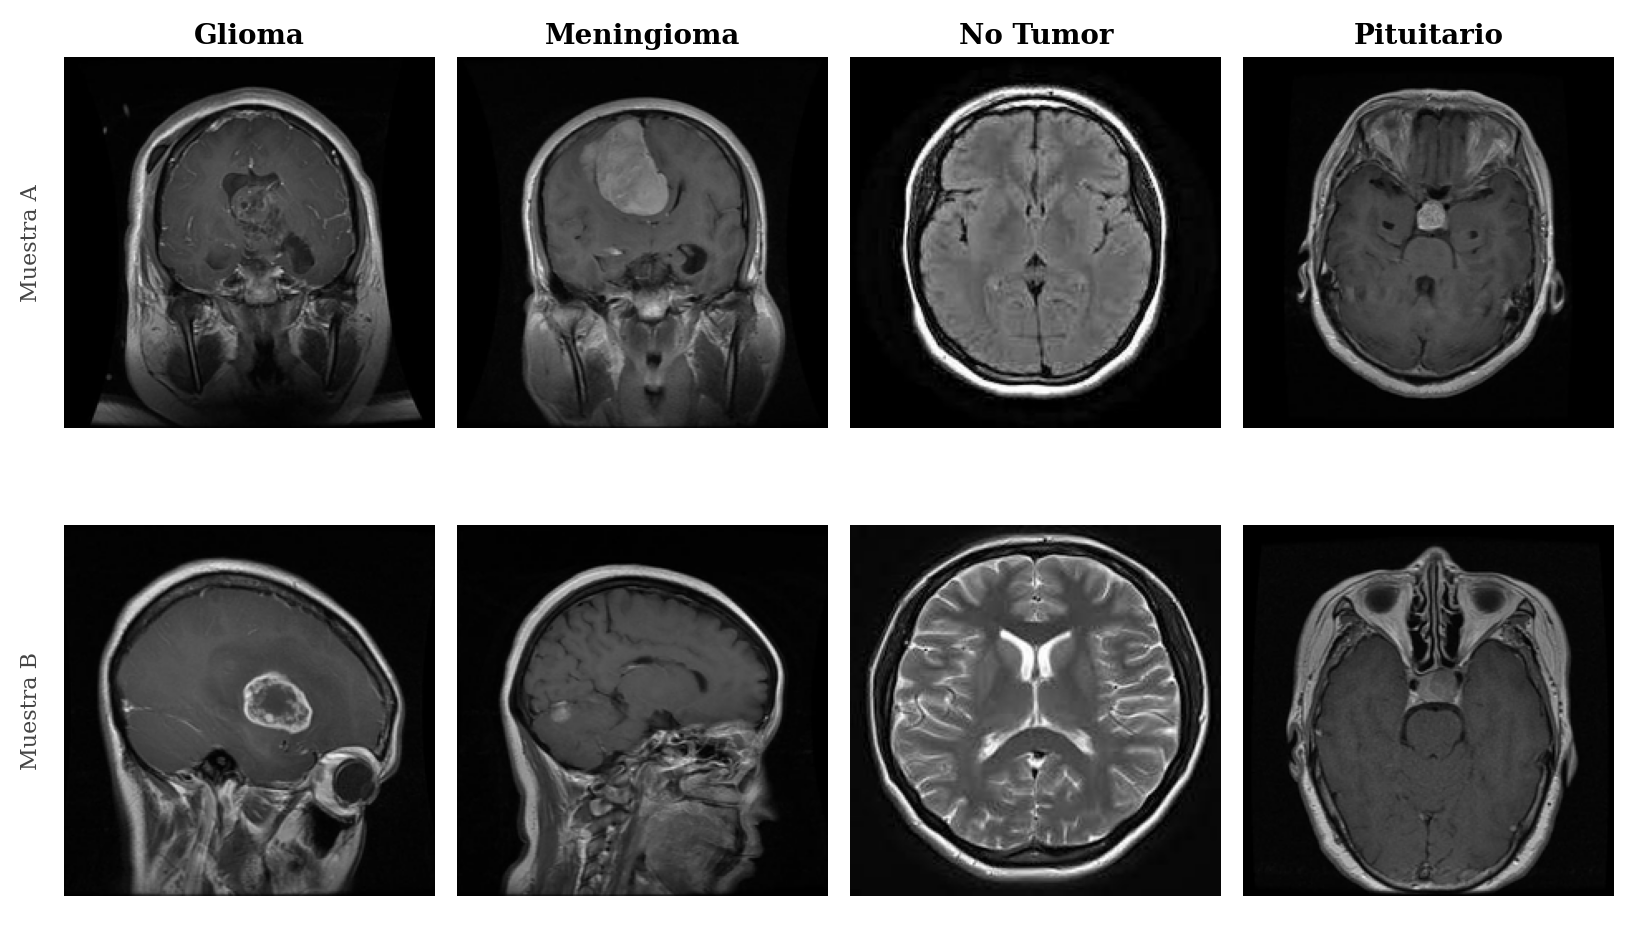
\includegraphics[width=\linewidth]{images/fig_brain_tumor_samples.png}
  \caption{Muestras representativas del dataset Brain Tumor MRI, ilustrando la variabilidad visual intra-clase e inter-clase entre las cuatro categorías diagnósticas.}
  \label{fig:fig_brain_tumor_samples}
  \vspace{0.2cm}
  \small Fuente: Kaggle Brain Tumor MRI Dataset \cite{msoud_nickparvar_2026}.
\end{figure}

\subsection{CIFAR-10}

CIFAR-10 se empleó como dataset de referencia estándar \cite{krizhevsky2009learning}. Contiene $60\,000$ imágenes de
$32 \times 32$ píxeles distribuidas en diez clases, con $50\,000$ imágenes de entrenamiento
y $10\,000$ de prueba. Todas las imágenes se redimensionaron a $224 \times 224$ para
mantener la misma resolución de entrada que en Brain Tumor MRI. El preprocesamiento incluyó
volteo horizontal aleatorio y normalización con las estadísticas propias del dataset. 
En test se aplicó únicamente redimensionamiento y normalización.


\begin{figure}[htbp]
  \centering
  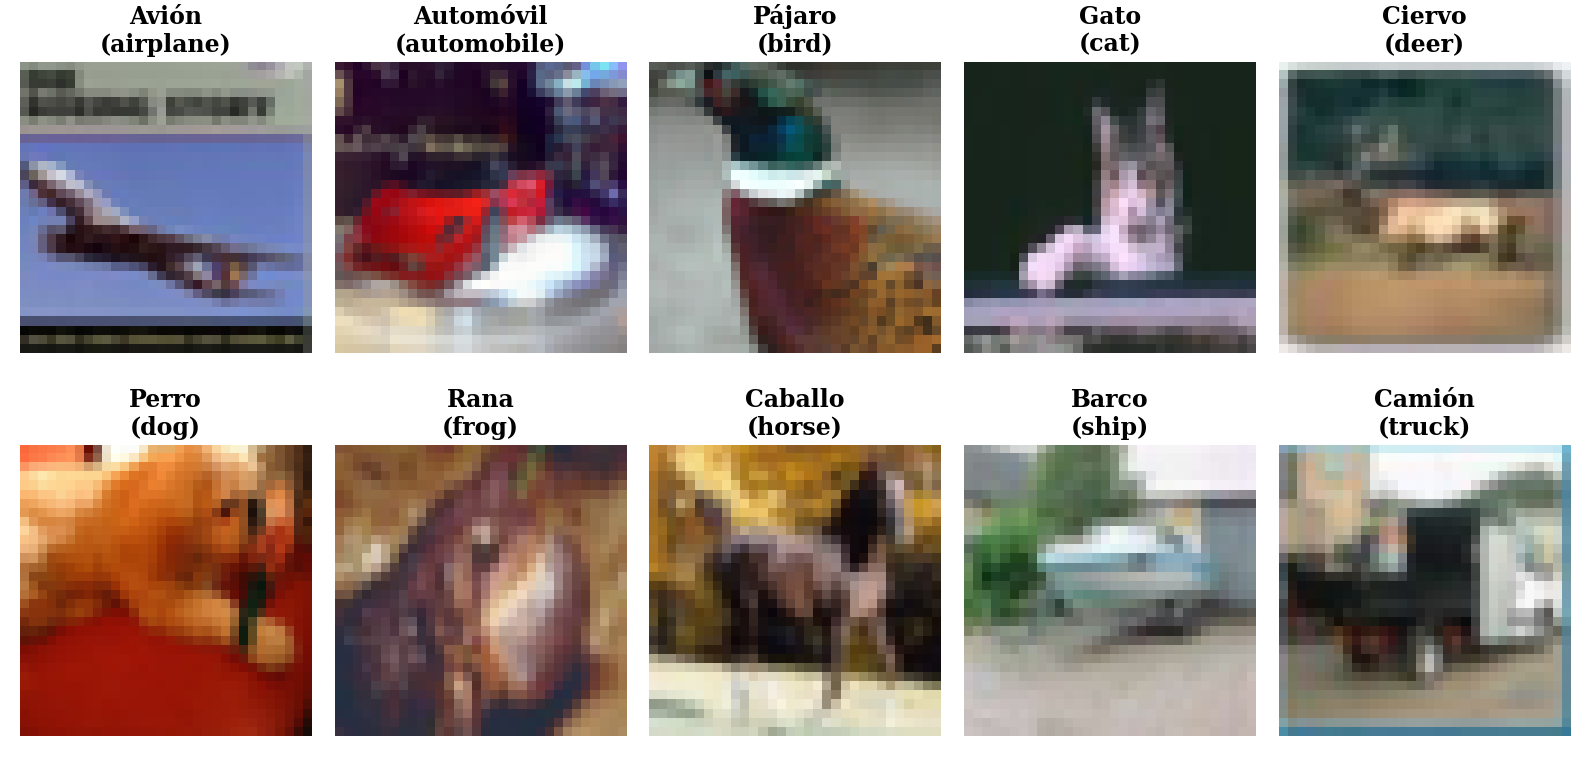
\includegraphics[width=\linewidth]{images/fig_cifar10_samples.png}
  \caption{Muestras representativas del dataset CIFAR-10 (una imagen por clase,
           resolución original $32\times32$ px). Las diez clases cubren objetos
           cotidianos de transporte, animales y vehículos.}
  \label{fig:fig_cifar10_samples}
  \vspace{0.2cm}
  \small Fuente: CIFAR-10 \cite{msoud_nickparvar_2026}.
\end{figure}



\subsection{Configuración del DataLoader}

En todos los experimentos se utilizó \texttt{DataLoader} con \texttt{batch\_size = 32},
\texttt{shuffle = True}, \texttt{num\_workers = 2} y \texttt{pin\_memory = True}. El
parámetro \texttt{drop\_last = True} fue obligatorio para los modelos con BatchNorm, ya que
un batch de tamaño unitario al final de una época local provoca una división por cero en el
cálculo de la varianza del batch.

% ============================================================
\section{Particionamiento Federado No-IID}
% ============================================================

\subsection{Estrategia Dirichlet}

La heterogeneidad estadística entre clientes se generó mediante particiones de Dirichlet
sobre las etiquetas de entrenamiento. Para $C$ clases y $K = 10$ clientes, se muestreó un
vector de proporciones $\mathbf{q}_k \sim \text{Dir}(\alpha \cdot \mathbf{1}_C)$ por clase y
se asignó a cada cliente $k$ la fracción $q_{k,c}$ de las muestras de la clase $c$. Cuando
algún cliente recibía menos de diez muestras de una clase asignada, se aplicó un paso de
redistribución para garantizar ese mínimo.

Se evaluaron cinco niveles de heterogeneidad: $\alpha \in \{1000, 1.0, 0.3, 0.1, 0.03\}$, 
siguiendo una configuración similar propuesta por \cite{jimenez2503thorough}.
El valor $\alpha = 1000$ produce una partición prácticamente IID; $\alpha = 0.03$ concentra
la mayoría de las muestras de cada clase en uno o dos clientes. La Tabla~\ref{tab:alpha_levels}
resume la correspondencia entre $\alpha$ y el nivel de heterogeneidad.

\begin{table}[H]
\centering
\caption{Niveles de heterogeneidad evaluados según el parámetro $\alpha$ de Dirichlet.}
\label{tab:alpha_levels}
\begin{tabular}{cll}
\hline
$\alpha$ & Nivel & Distancia de Hellinger aproximada \\
\hline
1000  & IID (línea base) & $\approx 0.00$ \\
1.0   & Baja             & $\approx 0.50$ \\
0.3   & Moderada         & $\approx 0.65$ \\
0.1   & Alta             & $\approx 0.80$ \\
0.03  & Extrema          & $\approx 0.90$ \\
\hline
\end{tabular}
\end{table}


\begin{figure}[htbp]
  \centering
  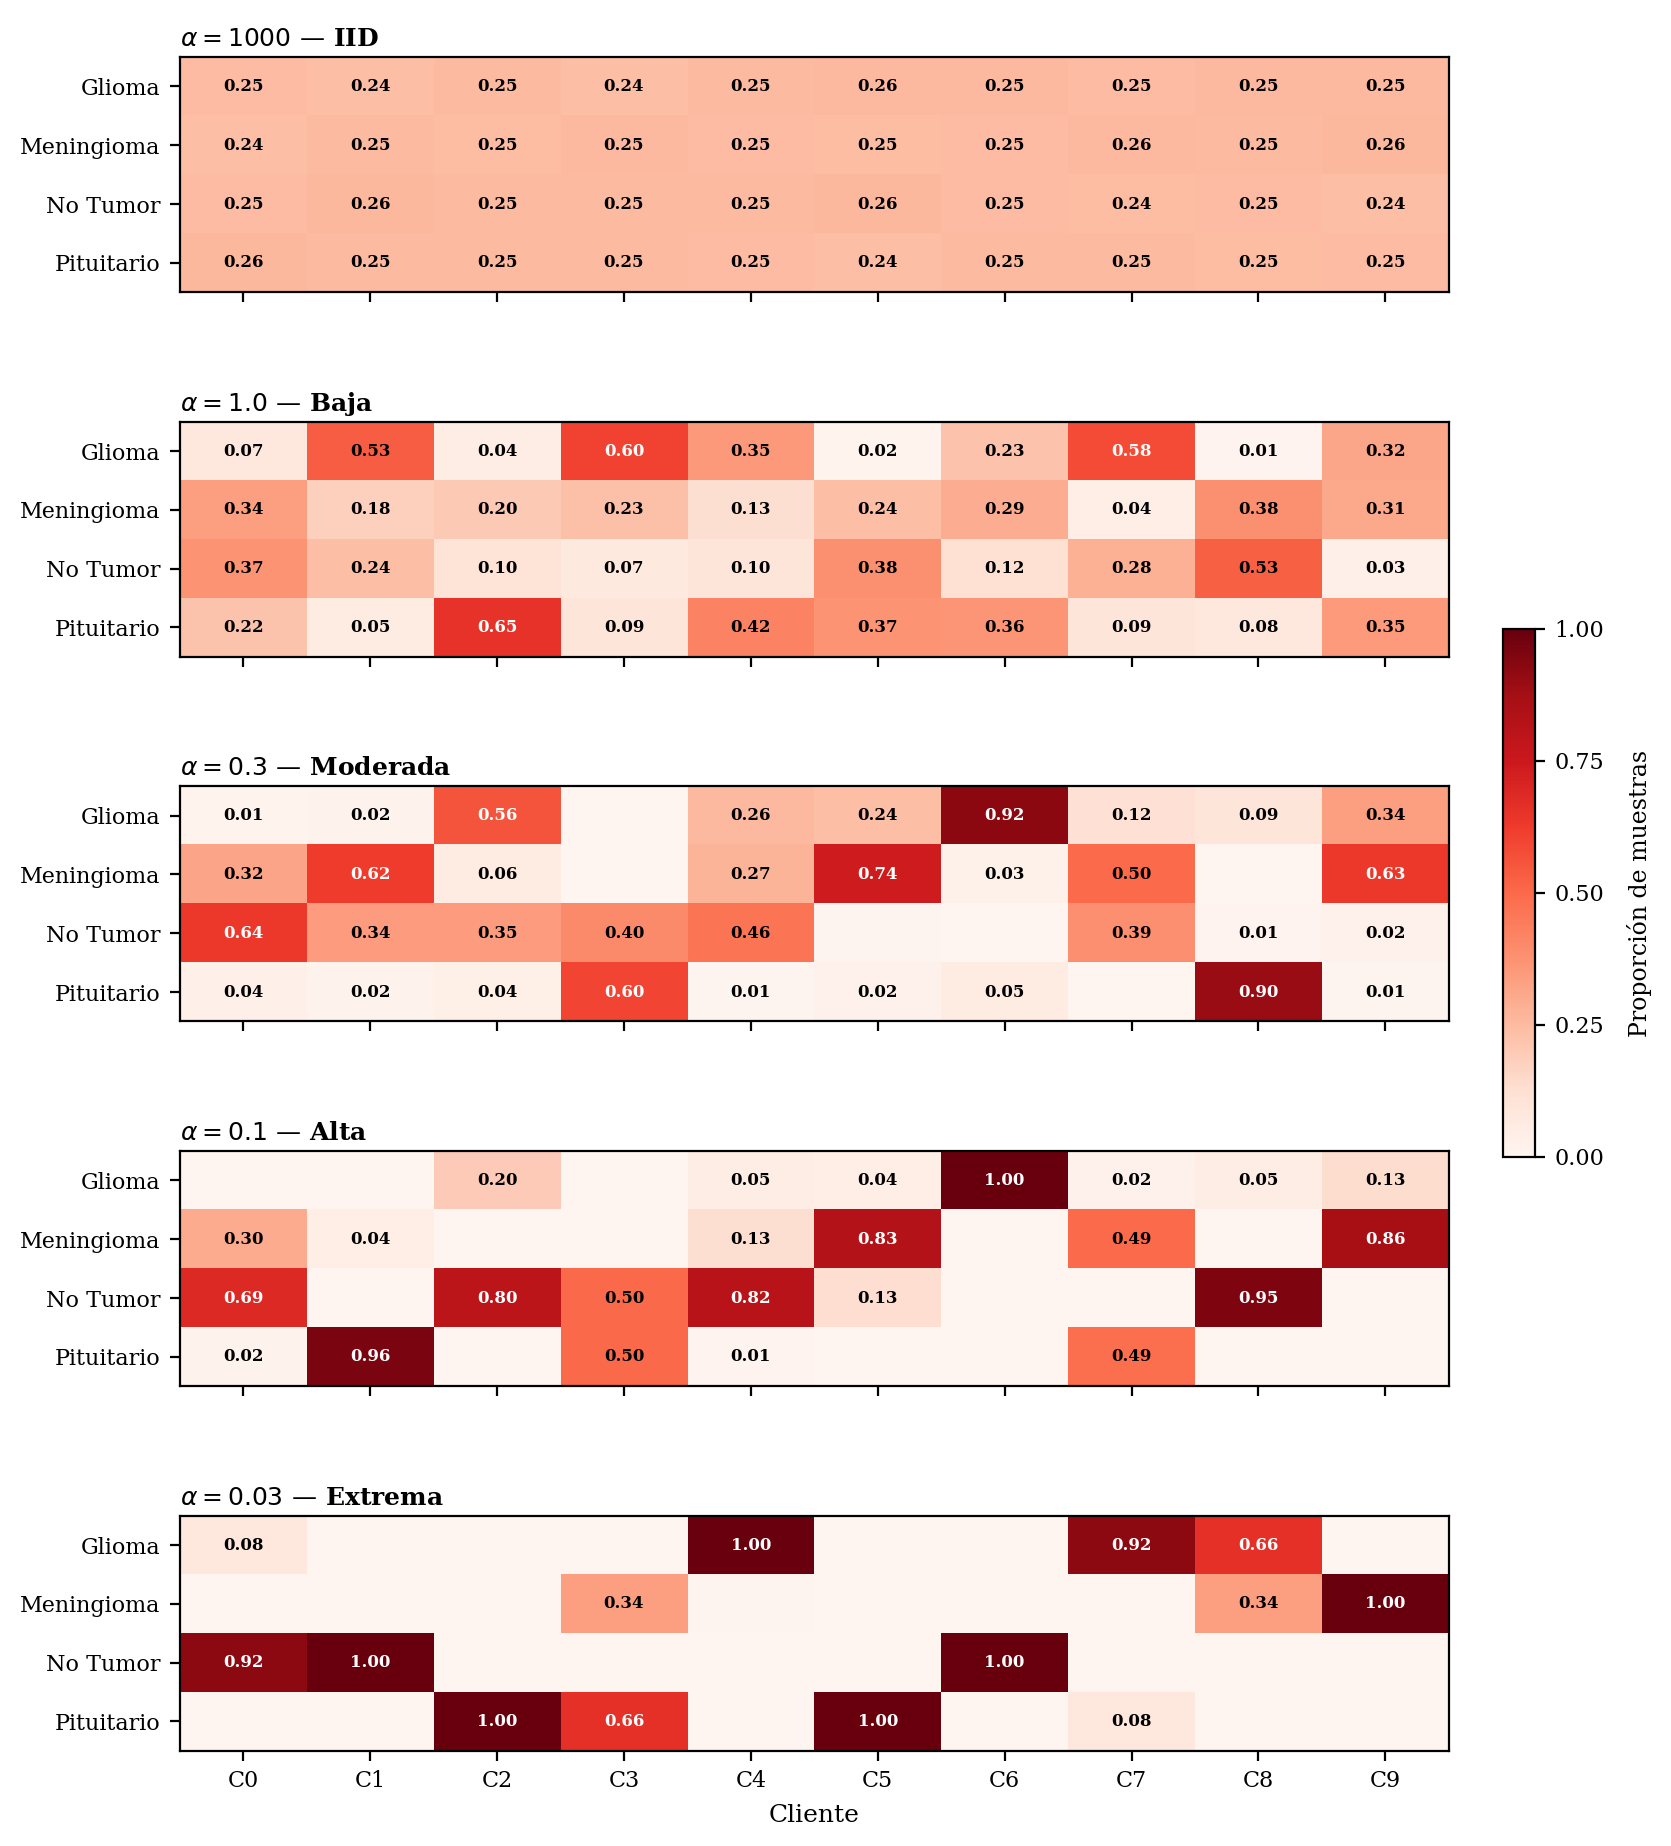
\includegraphics[width=\linewidth]{images/fig_dirichlet_partitions.png}
  \caption[Particiones Dirichlet — Brain Tumor MRI]{%
    Distribución de etiquetas por cliente bajo particiones
    Dirichlet para cinco niveles de heterogeneidad ($K=10$, semilla 42).
    Cada celda indica la proporción de muestras de esa clase asignadas al cliente.
    A medida que $\alpha$ decrece, la concentración por clase aumenta y la
    variabilidad inter-cliente se amplifica.}
  \label{fig:fig_dirichlet_partitions}

\end{figure}


\subsection{Reproducibilidad de las particiones}

Cada partición se generó con una semilla fija mediante \texttt{generate\_data.py} y se
almacenó en \path{data/{dataset}/partitions/alpha_{a}/seed_{seed}/}.
Cada directorio contiene \texttt{partition.pkl} con los índices por cliente y
\texttt{all\_stats.json} con la distribución de etiquetas, entropía y Distancia de Hellinger
por cliente. El uso de la misma semilla garantiza particiones idénticas entre modelos y
algoritmos, de modo que las diferencias observadas en el drift son atribuibles a la
arquitectura y no a variaciones en los datos.

El conjunto de prueba no se particionó: todos los clientes y el servidor evalúan sobre el
mismo test global, lo que permite comparar el rendimiento de generalización sin ambigüedad.

% ============================================================
\section{Modelos Evaluados}
% ============================================================

\subsection{Especificaciones de las arquitecturas}

Se evaluaron siete variantes de modelo pertenecientes a cuatro familias arquitectónicas.
La Tabla~\ref{tab:models} resume sus especificaciones principales. Todos los modelos se
inicializaron con pesos aleatorios para aislar el efecto
de la arquitectura sobre el drift sin confundir con representaciones preaprendidas. Esta
decisión implica una convergencia más lenta y una precisión final menor que con
preentrenamiento, en particular sobre Brain Tumor MRI (${\sim}7\,000$ imágenes); los
resultados deben interpretarse como medición del comportamiento de drift arquitectónico
bajo federación y no como benchmarks de clasificación absolutos.

\begin{table}[H]
\centering
\caption{Especificaciones de los siete modelos evaluados.}
\label{tab:models}
\resizebox{\textwidth}{!}{%
\begin{tabular}{llllll}
\hline
Modelo & Clave & Familia & Normalización & Dim. emb. & Bloques \\
\hline
EfficientNet-B1 (BN) & \texttt{efficient1}     & CNN & BatchNorm2d            & --- & 8 etapas \\
EfficientNet-B1 (GN) & \texttt{efficient1\_gn} & CNN & GroupNorm-32           & --- & 8 etapas \\
EfficientNet-B1 (LN) & \texttt{efficient1\_ln} & CNN & GroupNorm-1 ($\equiv$ LN) & --- & 8 etapas \\
ViT-Tiny             & \texttt{vit\_tiny}      & ViT & LayerNorm              & 192 & 12 bloques Transformer \\
Vim-Tiny             & \texttt{vim\_tiny}      & SSM & RMSNorm (fusionado)    & 192 & 12 bloques SSM \\
ViG-Tiny             & \texttt{vig\_tiny}      & GNN & BatchNorm2d            & 192 & 12 bloques Grapher \\
ResNet-9             & \texttt{res9}           & CNN & BatchNorm2d            & --- & 4 etapas + 2 res. \\
\hline
\end{tabular}}
\end{table}

\begin{center}
\textit{[FIGURA M5: Diagramas de bloque de las cuatro familias arquitectónicas evaluadas]}\\
\textit{Descripción: Cuatro paneles, uno por familia. (a) EfficientNet-B1: bloque MBConv con}
\textit{convolución depthwise + SE, con las capas de normalización indicadas en color.}
\textit{(b) ViT-Tiny: bloque Transformer con MHSA y MLP, LayerNorm en posición pre-norm.}
\textit{(c) Vim-Tiny: bloque SSM bidireccional con escaneo forward/backward y RMSNorm.}
\textit{(d) ViG-Tiny: bloque Grapher con construcción del grafo $k$-NN y propagación de mensajes.}
\textit{En cada panel se indica el número de bloques, la dimensión de embedding y la normalización.}
\textit{Propósito: mostrar en una sola figura las diferencias estructurales entre familias que}
\textit{determinan los distintos sesgos inductivos y perfiles de drift.}\\
\textit{Fuente: elaboración propia, basada en las referencias originales de cada arquitectura.}
\end{center}

\subsection{Ablación de normalización sobre EfficientNet-B1}

Las tres variantes de EfficientNet comparten exactamente el mismo sesgo inductivo
convolucional —bloques MBConv, módulos Squeeze-and-Excitation y jerarquía de
características— y difieren únicamente en la estrategia de normalización. La función
\texttt{replace\_batchnorm()} sustituyó recursivamente todos los módulos
\texttt{BatchNorm2d} por \texttt{GroupNorm(32)} o \texttt{GroupNorm(1)} $\equiv$
\texttt{LayerNorm} sobre la CNN base, preservando el número de parámetros aprendibles.
Esta ablación permite atribuir las diferencias de drift observadas entre variantes a la
normalización y no al mecanismo de extracción de características.

\subsection{Registro en FL-bench}

Como base de software para la experimentación se utilizó el repositorio
\textit{FL-bench} \cite{Tan_FL-bench}, un framework de
código abierto para la evaluación de algoritmos de aprendizaje federado. El repositorio
provee la infraestructura de comunicación cliente-servidor, la interfaz \texttt{DecoupledModel},
los algoritmos FedAvg y FedProx, y el pipeline de entrenamiento federado sobre el que se
construyeron todas las extensiones de este trabajo (registro de métricas de drift, cómputo
offline de CKA y scheduler del lado del servidor).

Todos los modelos se registraron en el diccionario \texttt{MODELS} de
\texttt{src/utils/models.py}, heredando de \texttt{DecoupledModel} y definiendo
\texttt{self.base} (extractor de características) y \texttt{self.classifier} (cabeza de
clasificación). ViG-Tiny se importa desde \texttt{Vision\_GNN/} mediante inyección de
\texttt{sys.path} en el momento de la construcción; el wrapper \texttt{\_ViGBase} sirve
únicamente para satisfacer la interfaz de \texttt{DecoupledModel}. Vim-Tiny requiere
\texttt{mamba\_ssm} con kernels CUDA fusionados; la importación está protegida por un
bloque \texttt{try/except} con mensaje de error informativo.

% ============================================================
\section{Protocolo de Aprendizaje Federado}
% ============================================================

\subsection{Configuración experimental}

La Tabla~\ref{tab:fl_config} resume los hiperparámetros del protocolo federado, comunes a
todos los experimentos. Se empleó una topología \textit{cross-silo} con $K = 10$ clientes
de participación completa en cada ronda, eliminando el ruido de muestreo del análisis de
drift. El número de rondas se fijó en $T = 50$ para observar tanto la dinámica temprana del
drift (rondas 1--10) como el comportamiento de convergencia tardía.

\begin{table}[H]
\centering
\caption{Hiperparámetros del protocolo federado.}
\label{tab:fl_config}
\begin{tabular}{ll}
\hline
Parámetro                        & Valor \\
\hline
Número de clientes ($K$)         & 10 \\
Participación por ronda          & 1.0 (100\%) \\
Rondas de comunicación ($T$)     & 50 \\
Épocas locales ($E$)             & 5 \\
Tamaño de batch ($B$)            & 32 \\
Optimizador                      & SGD (momentum $= 0.9$, wd $= 10^{-4}$) \\
Tasa de aprendizaje inicial      & 0.01 \\
Scheduler de LR                  & CosineAnnealingLR (lado servidor) \\
$\mu$ FedProx                    & 0.01 \\
Semillas                         & 42, 123, 456 \\
\hline
\end{tabular}
\end{table}

El scheduler de tasa de aprendizaje se implementó del lado del servidor para garantizar
que todos los clientes inicien cada ronda con el mismo LR globalmente decaído. FL-bench
avanza el scheduler una vez por época local, lo que produciría $E = 5$ veces más pasos que
los deseados. El servidor calcula el LR coseno correspondiente a la ronda $t$ e inyecta el
valor en \texttt{args.optimizer.lr}; los clientes construyen su optimizador con ese valor
al inicio de cada ronda (\texttt{reset\_optimizer\_on\_global\_epoch: true}).

\subsection{Ciclo de una ronda de comunicación}

El protocolo de cada ronda $t$ siguió los siguientes pasos:

\begin{enumerate}
  \item El servidor difunde el modelo global $\boldsymbol{\theta}^{(t-1)}$ a los $K$
    clientes.
  \item Cada cliente $k$ ejecuta $E$ épocas de SGD local sobre $\mathcal{D}_k$, obteniendo
    $\boldsymbol{\theta}_k^{(t)}$.
  \item \textbf{Antes de la agregación}: el servidor registra el drift $L_2$ por grupo de
    capas y la similitud coseno inter-cliente para cada par de clientes.
  \item El servidor agrega: $\boldsymbol{\theta}^{(t)} = \sum_k (n_k/n)\,
    \boldsymbol{\theta}_k^{(t)}$.
  \item \textbf{Después de la agregación}: el servidor evalúa accuracy y F1 sobre el test
    global y registra equidad inter-cliente.
  \item En las rondas de checkpoint programadas $\{1, 2, 5, 10, 20, 30, 40, 50\}$, se
    guardan el estado del modelo global pre-agregación y los estados de todos los clientes
    post-entrenamiento, para el cómputo offline de CKA.
\end{enumerate}

\begin{center}
\textit{[FIGURA M6: Diagrama de flujo de una ronda de comunicación federada]}\\
\textit{Descripción: Diagrama vertical con cinco bloques secuenciales: (1) broadcast del}
\textit{modelo global a los 10 clientes; (2) entrenamiento local paralelo en cada cliente}
\textit{($E=5$ épocas de SGD); (3) registro de métricas de drift ANTES de la agregación;}
\textit{(4) agregación FedAvg/FedProx en el servidor; (5) evaluación global y guardado de}
\textit{checkpoint condicional. Las ramas de FedAvg y FedProx se distinguen en el bloque (4).}
\textit{Propósito: mostrar con precisión el orden de las operaciones en cada ronda, en especial}
\textit{la posición del registro de métricas respecto a la agregación.}\\
\textit{Fuente: elaboración propia.}
\end{center}

% ============================================================
\section{Taxonomía de Capas para el Análisis de Drift}
% ============================================================

Para hacer comparables las métricas de drift entre familias arquitectónicas con estructuras
internas heterogéneas, los parámetros de cada modelo se clasificaron en tres grupos
funcionales mediante la función \texttt{classify\_layer(name, module)} implementada en
\texttt{src/utils/drift\_metrics.py}:

\begin{itemize}
  \item \textbf{norm}: parámetros aprendibles ($\gamma$, $\beta$) de las capas de
    normalización (BatchNorm2d, GroupNorm, LayerNorm, RMSNorm).
  \item \textbf{feature}: pesos de las capas de extracción de características
    (Conv2d, proyecciones lineales internas), excluida la cabeza clasificadora.
  \item \textbf{head}: parámetros de la capa clasificadora final.
\end{itemize}

Los buffers de BatchNorm (\texttt{running\_mean}, \texttt{running\_var},
\texttt{num\_batches\_tracked}) se excluyen del cómputo, ya que no participan en la
agregación FedAvg. Los módulos de activación y pooling se clasifican como \texttt{other}
y quedan fuera de todas las métricas de drift.

La Tabla~\ref{tab:layer_taxonomy} especifica la correspondencia entre esta taxonomía y los
módulos concretos de cada arquitectura.

\begin{table}[H]
\centering
\caption{Taxonomía de capas por arquitectura.}
\label{tab:layer_taxonomy}

\begin{tabularx}{\textwidth}{l l X l}
\hline
Arquitectura & \textbf{norm} & \textbf{feature} & \textbf{head} \\
\hline
EfficientNet-B1 & BN / GN / LN layers & Bloques MBConv (Conv2d, SE) & FC clasificador \\
ViT-Tiny & LayerNorm layers & Atención (Q, K, V) + MLP & Proj. sobre [CLS] \\
Vim-Tiny & RMSNorm layers & Proyecciones SSM (B, C, $\Delta$) & FC clasificador \\
ViG-Tiny & BN layers & Bloques Grapher + FFN & FC clasificador \\
ResNet-9 & BN layers & Conv2d, bloques residuales & FC clasificador \\
\hline
\end{tabularx}
\end{table}

% ============================================================
\section{Métricas de Drift Paramétrico}
% ============================================================

\subsection{\texorpdfstring{Divergencia de pesos $L_2$}{Divergencia de pesos L2} por grupo de capas}

Para cada cliente $k$, grupo de capas $\ell \in \{\text{norm, feature, head}\}$ y ronda
$t$, se calcularon dos variantes complementarias de drift:

\textbf{Drift crudo} (escala-dependiente):
\begin{equation}
  \text{drift\_raw}_k^{(\ell)}(t) =
  \left\|\boldsymbol{\theta}_k^{(\ell)}(t) - \boldsymbol{\theta}_{\text{global}}^{(\ell)}
  (t-1)\right\|_2.
  \label{eq:drift_raw}
\end{equation}

\textbf{Drift normalizado RMS} (escala-independiente):
\begin{equation}
  \text{drift\_norm}_k^{(\ell)}(t) =
  \frac{\text{drift\_raw}_k^{(\ell)}(t)}{\sqrt{N^{(\ell)}}},
  \label{eq:drift_norm}
\end{equation}

donde $N^{(\ell)}$ es el número total de parámetros escalares en el grupo $\ell$. Esta
normalización convierte el valor en el drift RMS por parámetro, permitiendo comparaciones
directas entre grupos de tamaños muy distintos y entre arquitecturas. Todas las comparaciones
cross-arquitectura de este trabajo emplean \texttt{drift\_norm}; el drift crudo se retiene
para verificar que el término proximal de FedProx acota la magnitud absoluta esperada.

Para cada ronda se reportan la media y desviación estándar del drift normalizado sobre los
$K = 10$ clientes, por grupo de capas.

\subsection{Alineación de gradientes inter-cliente}

La similitud coseno pairwise por grupo de capas y ronda cuantifica si las actualizaciones
de distintos clientes son constructivas o destructivas al ser promediadas:

\begin{equation}
  \text{alignment}^{(\ell)}(t) = \frac{1}{K(K-1)}
  \sum_{i=1}^{K} \sum_{j \neq i}
  \frac{\mathbf{g}_i^{(\ell)}(t) \cdot \mathbf{g}_j^{(\ell)}(t)}
  {\left\|\mathbf{g}_i^{(\ell)}(t)\right\|_2 \left\|\mathbf{g}_j^{(\ell)}(t)\right\|_2},
  \label{eq:cosine}
\end{equation}

donde $\mathbf{g}_k^{(\ell)}(t) = \boldsymbol{\theta}_{\text{global}}^{(\ell)}(t-1) -
\boldsymbol{\theta}_k^{(\ell)}(t)$ es el pseudo-gradiente del cliente $k$ en el grupo
$\ell$. Valores positivos indican actualizaciones constructivas; valores negativos,
interferencia destructiva.

Ambas métricas se registran \textit{antes} de la agregación en cada ronda, en
\texttt{DriftFedAvgServer.aggregate\_client\_updates()} y su análogo para FedProx, y se
almacenan en \texttt{drift\_metrics.csv}.

\begin{center}
\textit{[FIGURA M7: Pipeline de registro de métricas paramétricas durante el entrenamiento]}\\
\textit{Descripción: Diagrama de flujo detallado del interior del bloque de agregación de la}
\textit{Figura M6. Muestra la secuencia: (1) recepción de los $K$ state dicts de clientes;}
\textit{(2) cálculo de drift raw y norm para cada cliente y grupo de capas; (3) cálculo de}
\textit{similitud coseno pairwise para cada grupo; (4) escritura en \texttt{drift\_metrics.csv};}
\textit{(5) guardado de checkpoints condicional (rondas programadas); (6) promedio FedAvg/FedProx.}
\textit{Propósito: documentar el orden exacto de las operaciones y el punto de captura de datos,}
\textit{garantizando la trazabilidad del momento de medición respecto a la agregación.}\\
\textit{Fuente: elaboración propia.}
\end{center}

% ============================================================
\section{Análisis de Representaciones mediante CKA}
% ============================================================

\subsection{Arquitectura del pipeline offline}

El cómputo de CKA se desacopló completamente del entrenamiento para eliminar la presión sobre
la memoria GPU. El flujo se divide en dos etapas diferenciadas:

\textbf{Durante el entrenamiento} (\texttt{CKADriftFedAvgServer}): en las rondas programadas
$\{1, 2, 5, 10, 20, 30, 40, 50\}$, el servidor guarda en disco el estado del modelo global
pre-agregación (\texttt{global.pt}) y el estado de cada cliente post-entrenamiento local
(\texttt{client\_k.pt}), junto con los metadatos del experimento (\texttt{run\_metadata.json}).
No se realizan forward passes ni cálculos de activaciones durante el entrenamiento.

\textbf{Después del entrenamiento} (scripts offline en \texttt{scripts/}):
\begin{itemize}
  \item \texttt{compute\_cka\_offline.py}: calcula el CKA global-vs-cliente para cada ronda
    programada y guarda los resultados en \texttt{cka\_metrics.csv} y matrices completas en
    \texttt{cka\_matrices/*.npz}.
  \item \texttt{compute\_client\_cka\_offline.py}: calcula el CKA pairwise entre todos los
    pares de clientes y guarda en \texttt{client\_cka\_metrics.csv}.
\end{itemize}

\begin{center}
\textit{[FIGURA M8: Pipeline CKA — fases durante y después del entrenamiento]}\\
\textit{Descripción: Diagrama de dos columnas. Columna izquierda (durante entrenamiento):}
\textit{el servidor entrena T=50 rondas; en las rondas programadas $\{1,2,5,10,20,30,40,50\}$}
\textit{guarda checkpoints (global.pt + client\_k.pt) sin interrumpir el entrenamiento.}
\textit{Columna derecha (post-entrenamiento): los scripts offline leen los checkpoints,}
\textit{ejecutan forward passes en CPU, calculan CKA y escriben los CSV de resultados.}
\textit{Propósito: documentar la separación entre el entrenamiento y el análisis representacional,}
\textit{justificando la decisión de diseño que evita presión sobre la memoria GPU.}\\
\textit{Fuente: elaboración propia.}
\end{center}

\subsection{Mapa de capas por arquitectura}

Los puntos de hook para la recolección de activaciones se determinaron a partir de los
nombres exactos de los módulos expuestos por \texttt{named\_modules()}, ya que la lógica de
registro de hooks se implementó con coincidencia exacta de nombre. La
Tabla~\ref{tab:cka_layers} resume el número de capas monitoreadas por modelo.

\begin{table}[H]
\centering
\caption{Capas monitoreadas para CKA por arquitectura.}
\label{tab:cka_layers}

\begin{tabularx}{\textwidth}{l c X}
\hline
Modelo & $N_{\text{capas}}$ & Observaciones \\
\hline

EfficientNet-B1 (×3) & 10 &
\texttt{base.features.0--8} + \texttt{classifier} \\

ViT-Tiny & 15 &
\texttt{base.patch\_embed} + \texttt{base.blocks.0--11} +
\texttt{base.norm} + \texttt{classifier} \\

Vim-Tiny & 14 &
\texttt{base.patch\_embed} + \texttt{base.layers.0--11.mixer} +
\texttt{classifier} \newline
(capas norm excluidas: kernel CUDA fusionado no dispara hook) \\

ViG-Tiny & 14 &
\texttt{\_vig\_stem} + \texttt{\_vig\_blocks.0--11} +
\texttt{classifier} \newline
(módulos en raíz del objeto, no bajo \texttt{self.base}) \\

ResNet-9 & 9 &
\texttt{base.2}, \texttt{base.6}, \texttt{base.7},
\texttt{base.11}, \texttt{base.15--18} +
\texttt{classifier} \\

\hline
\end{tabularx}
\end{table}

\subsection{Análisis CKA global-vs-cliente}

Para cada ronda programada $t$ y cliente $k$, se cargaron \texttt{global.pt} y
\texttt{client\_k.pt}, se hicieron pasar $N_{\text{probe}} \leq 512$ muestras por ambos
modelos en CPU y se calculó el CKA diagonal entre las activaciones de capas homólogas:

\begin{equation}
  \text{CKA\_gc}_{k}^{(\ell)}(t) = \text{CKA}\!\left(
    \mathbf{X}_{k}^{(\ell)}(t),\; \mathbf{X}_{\text{global}}^{(\ell)}(t)
  \right),
  \label{eq:cka_gc}
\end{equation}

donde $\mathbf{X}_{k}^{(\ell)}$ y $\mathbf{X}_{\text{global}}^{(\ell)}$ son las matrices de
activación de la capa $\ell$ evaluadas sobre el mismo conjunto de muestras de referencia.
Un valor cercano a 1 indica que el cliente conserva representaciones funcionalmente alineadas
con el modelo global; un valor cercano a 0 indica divergencia representacional.

\subsection{Análisis CKA pairwise inter-cliente}

Para cada par de clientes $(i, j)$ y ronda programada $t$, se calculó el CKA entre sus
activaciones sobre las mismas muestras de referencia. Este análisis complementa el
global-vs-cliente al cuantificar si distintos clientes están aprendiendo representaciones
similares entre sí, independientemente del modelo global.

\subsection{Gestión de memoria}

Los forward passes de CKA se ejecutaron en CPU. Las activaciones espaciales (tensores 4D)
se redujeron a 2D mediante pooling global antes del almacenamiento en RAM. Se limitó el
número de muestras de sondeo a 512 filas por capa, lo que es suficiente para estimados CKA
estables según \cite{DBLP:journals/corr/abs-1905-00414}. Los parámetros
\texttt{probe\_batches = 20} y \texttt{probe\_batch\_size = 16} se registraron en
\texttt{run\_metadata.json} para garantizar la reproducibilidad del análisis offline.

% ============================================================
\section{Métricas de Evaluación del Rendimiento}
% ============================================================

\subsection{Métricas de clasificación}

Tras cada ronda de comunicación se evaluó el modelo global sobre el test global y se
calcularon accuracy, F1-score macro, precision macro y recall macro. El F1-score macro es la
métrica primaria para Brain Tumor MRI por su robustez ante variaciones en la distribución
de clases bajo particiones Dirichlet; la
accuracy es la métrica primaria para CIFAR-10.

\subsection{Velocidad de convergencia}

La convergencia se definió como la primera ronda $t$ en que la accuracy global cruza el
umbral establecido —70\,\% para CIFAR-10 y 80\,\% para Brain Tumor MRI— y permanece por
encima durante cinco rondas consecutivas. Los modelos que no alcanzaron la convergencia en
$T = 50$ rondas se registraron con \texttt{convergence\_round = -1}.

\subsection{Equidad inter-cliente}

La equidad se midió como la brecha de accuracy entre el cliente con mayor y menor rendimiento
al final del entrenamiento (\textit{fairness gap}). Como indicador secundario se reportó la
desviación estándar de accuracy entre los diez clientes.

\subsection{Agregación estadística}

Todos los resultados se reportan como $\mu \pm \sigma$ sobre las tres semillas $\{42, 123,
456\}$. Las ejecuciones con desviación estándar de accuracy superior a $0.03$ se marcaron
como alta varianza para inspección adicional. Para las comparaciones clave entre
arquitecturas se aplicó la prueba de Wilcoxon signed-rank (no paramétrica, $\alpha = 0.05$).
Dado el tamaño de muestra reducido ($n = 3$ semillas), los $p$-values se reportan como
indicativos y no definitivos.

% ============================================================
\section{Estudios de Ablación}
% ============================================================

Se diseñaron cinco estudios de ablación para aislar los factores de mayor interés. Los tres
primeros son primarios y forman parte del análisis principal; los dos últimos son secundarios.

\textbf{Ablación 1 — Normalización.} Se compararon EfficientNet-B1 en sus tres variantes (BN,
GN-32, LN) bajo configuración FL idéntica. El gap en drift, accuracy y CKA entre variantes
cuantifica la contribución específica de BatchNorm frente al sesgo inductivo convolucional.

\textbf{Ablación 2 — Heterogeneidad.} Para cada modelo se trazó la curva de accuracy vs.\
$\alpha$ sobre ambos datasets. El objetivo es identificar el valor crítico de $\alpha$ a
partir del cual el rendimiento de cada familia arquitectónica degrada de forma no lineal.

\textbf{Ablación 3 — Algoritmo federado.} Se compararon FedAvg y FedProx para cada
combinación modelo × dataset × $\alpha$, reportando las diferencias $\Delta_{\text{acc}}$,
$\Delta_{\text{drift}}$ y $\Delta_{\text{CKA}}$. La hipótesis es que FedProx beneficia
proporcionalmente más a las arquitecturas con mayor drift (BN-based).

\textbf{Ablación 4 — Intra-familia por normalización.} Se compararon los perfiles de drift L2
y CKA de los modelos con BatchNorm (EfficientNet-B1 BN, ViG-Tiny, ResNet-9) frente a los
modelos con normalización por muestra (ViT-Tiny, Vim-Tiny), independientemente de la familia.
Esta comparación separa el efecto de la normalización del efecto del sesgo inductivo.

\textbf{Ablación 5 — Épocas locales.} Se evaluaron $E \in \{1, 5, 10\}$ para una única
celda experimental ($\alpha = 0.1$, Brain Tumor MRI, FedAvg, semilla 42), con el objetivo de
verificar que el número de épocas locales amplifica el drift de forma diferenciada según
arquitectura.

% ============================================================
\section{Procedimiento Experimental}
% ============================================================

\begin{center}
\textit{[FIGURA M9: Diagrama general del procedimiento experimental]}\\
\textit{Descripción: Diagrama de flujo horizontal con nueve bloques secuenciales que}
\textit{representan las fases del experimento: (1) Configuración del entorno; (2) Preparación}
\textit{de datos y particionamiento; (3) Implementación de modelos; (4) Implementación de}
\textit{métricas de drift; (5) Implementación del pipeline CKA; (6) Ejecución de los 210 runs;}
\textit{(7) Verificación de integridad (50 filas por CSV, sanity check); (8) Análisis CKA}
\textit{offline; (9) Visualización y análisis estadístico. Las fases completadas se indican con}
\textit{una marca de verificación; las pendientes, con un reloj. Este diagrama refleja el estado}
\textit{real de avance al momento de la redacción.}\\
\textit{Fuente: elaboración propia.}
\end{center}

La ejecución experimental se organizó en nueve fases. Las fases 1 a 5 corresponden a la
preparación del entorno, la ingesta de datos, la implementación de modelos y la
instrumentación de métricas. La fase 6 ejecutó los 210 runs primarios: 7 modelos × 5 valores
de $\alpha$ × 3 semillas × 2 algoritmos sobre Brain Tumor MRI, con ejecuciones paralelas en
CIFAR-10 como referencia. La fase 7 verificó la integridad de los resultados mediante
\texttt{sanity\_check.py}, que detecta ejecuciones con accuracy final $< 0.1$, drift nulo o
alta varianza. Las fases 8 y 9 ejecutaron el análisis CKA offline y la generación de figuras.

La estructura de directorios de salida siguió el esquema:
\begin{center}
    \path{logs/runs/{dataset}_alpha{a}_{model}_{method}_seed{seed}/}
\end{center}

Cada directorio contiene: \texttt{drift\_metrics.csv} (50 filas, una por ronda),
\texttt{metrics.csv} (salida estándar de FL-bench), \texttt{main.log},
\texttt{events.out.tfevents.*} (TensorBoard), el subdirectorio \texttt{checkpoints/} con
los estados del modelo por ronda programada, y los ficheros CKA generados offline.

% ============================================================
\section{Infraestructura Tecnológica}
% ============================================================

\subsection{Hardware}

\textit{[COMPLETAR con: modelo de CPU, GPU (nombre, VRAM en GB), memoria RAM del sistema.]}

\subsection{Software}

\begin{table}[H]
\centering
\caption{Entorno de software utilizado.}
\label{tab:software}
\begin{tabular}{ll}
\hline
Componente              & Versión \\
\hline
Python                  & 3.11 \\
PyTorch                 & 2.6.0 \\
CUDA                    & \textit{[COMPLETAR]} \\
torchvision             & 0.21.0 \\
timm                    & 1.0.15 \\
vision-mamba / mamba\_ssm & 0.1.0 \\
scikit-learn            & 1.6.1 \\
numpy                   & 1.26.4 \\
pandas                  & 2.2.3 \\
matplotlib / seaborn    & 3.10.1 / 0.13.2 \\
TensorBoard             & 2.17.1 \\
\hline
\end{tabular}
\end{table}

La reproducibilidad del entorno se garantizó mediante \texttt{requirements\_locked.txt}
(salida de \texttt{pip freeze}) y \texttt{environment.txt} (versiones de CUDA, PyTorch y
especificaciones de GPU obtenidas mediante \texttt{nvidia-smi}), ambos archivos versionados
en el repositorio.

\input{secciones/capitulo4}
\input{secciones/conclusiones}
\input{secciones/recomendaciones} % sección opcional

%% ============================================================================
\renewcommand{\bibname}{\hfill\Large\bf{REFERENCIAS BIBLIOGRÁFICAS}\hfill}

\bibliographystyle{IEEEtran} % Estableciendo el estilo de citas IEEEtram.

\bibliography{referencias} % Recibe las referencias de IEEE

\input{secciones/anexos}

\end{document}
